\documentclass{article}

\usepackage[utf8]{inputenc}
\usepackage{polyglossia}
\setmainlanguage{russian}
\setotherlanguage{english}

\usepackage{fontspec}
\setmainfont{Liberation Serif}
\setsansfont{Liberation Sans}
\setmonofont{Liberation Mono}

\usepackage{import}
\usepackage{enumitem}
\usepackage{fancyhdr}
\usepackage{amsmath}
\usepackage{amsthm}
\usepackage{amsfonts}
\usepackage{graphicx}
\usepackage{geometry}
\usepackage[most]{tcolorbox}
\usepackage[
    backend=biber,
    style=ieee,
    sorting=ynt
]{biblatex}

\addbibresource{document.bib}
\selectlanguage{russian}
\geometry{a4paper,margin=1.75cm}
\newcommand{\mathdefault}[1][]{}
%
% Basic Document Settings
%

\pagestyle{fancy}
\fancyhf{}
\lhead{}
\chead{\docClass: \docTitle}
\cfoot{\thepage}

\renewcommand\headrulewidth{0.4pt}
\renewcommand\footrulewidth{0.4pt}

\setlength\parindent{0pt}

\newcommand{\docTitle}{Измерение функции нелинейности звукоснимателя}
\newcommand{\docClass}{Вопрос по выбору}
\newcommand{\docAuthorName}{
    \textbf{Циммерман Сергей} \textit{Б01--110}\\
    \textbf{Романов Александр} \textit{Б01--110}\\
}

%
% Title Page
%

\title{
    \vspace{2in}
    \textmd{\textbf{\docClass:\ \docTitle}}\\
    \vspace{3in}
}

\author{\docAuthorName}
\date{}

\begin{document}

\maketitle
\pagebreak

\section{Введение}

Электромагнтный звукосниматель (pickup) -- это электрический прибор, преобразующий механическое движение
струны в окрестности датчика в электрический сигнал. На характерное звучание электрических струнных инструментов
влияет множество факторов: материал и форма тела, тип струнодержателя, но наибольшую роль играет вид и положение звукоснимателя.
Как было показано теоретически \cite{acoustics-modeling-of-a-pickup} и экспериментально подтверждено \cite{novak:hal-02512148},
\cite{app7010050}, звукосниматель -- сильно нелинейный прибор, и нелинейные искажение определяют тембр и характер звучания.
В данной работе мы экспериментально исследуем нелинейность Humbucking звукоснимателя, пользуясь методами и установками,
доступными на кафедре Общей Физики в МФТИ.

\section{Принцип работы и модель}

Опишем физический принцип работы электромагнитного звукоснимателя.
Ключевыми компонентами являются:

\begin{enumerate}
    \item Постоянный магнит
    \item Катушка с достаточно большим числом витков
    \item Магнитно-проницаемая струна (обычно сталь или никель)
\end{enumerate}

\begin{figure}[h]
    \centering
    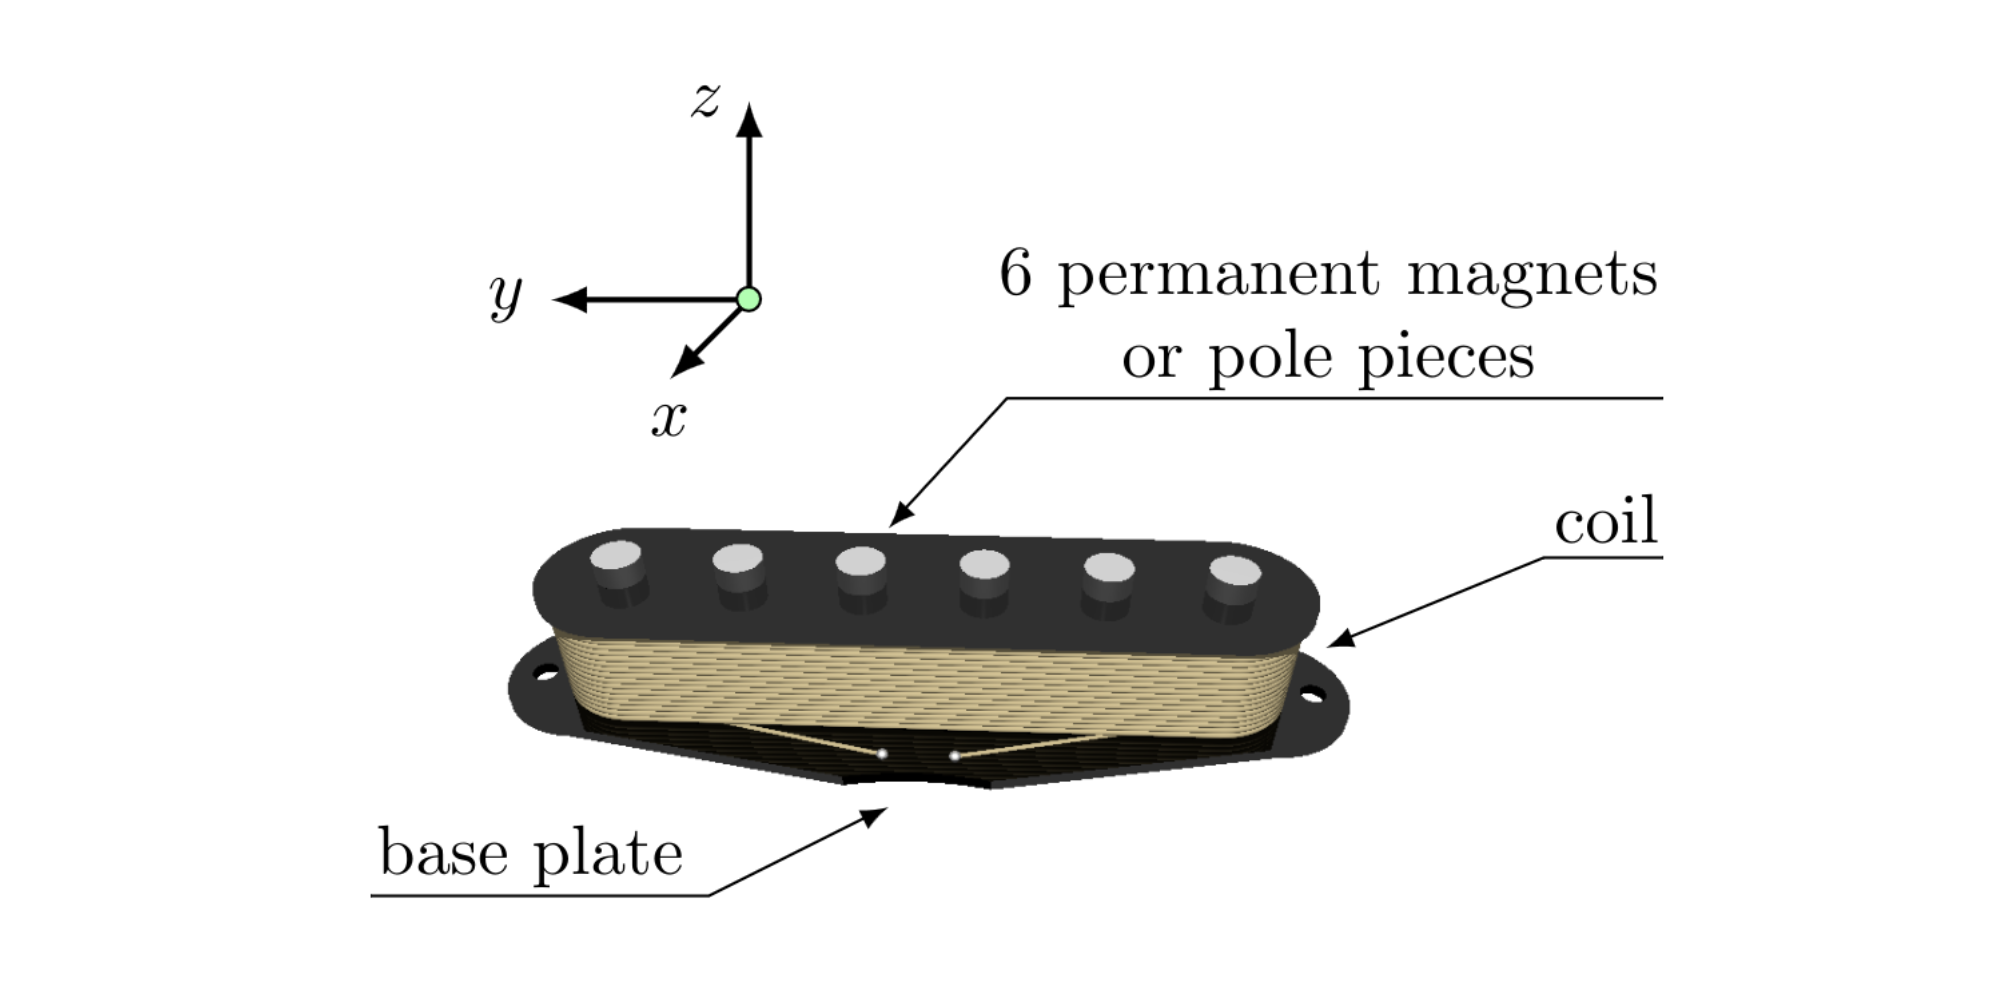
\includegraphics[width=8cm]{drawings/mechanism.png}
    \caption{Внутреннее устройство single-coil звукоснимателя}
\end{figure}

Струна, двигаясь во внешнем магнитном поле приобретает собственный магнитный момент.
Каждое достаточно тонкое цилиндрическое сечение струны можно рассматривать как диполь. В зависимости от положения струны
создается дополнительный переменный во времени магнитный поток, протекающий через катушку. В соотвествии с законом
электромагнитной индукции в катушке возникает ЭДС $\varepsilon = \frac{d\Phi}{dt}$. Таким образом, систему можно
представить в виде последовательности пространственной нелинейности $NL(y, z)$ и дифференцирования $d/dt$. Поставим задачу
измерить функцию $NL(z)\vert_{y = const}$, которая на самом деле является завимимостью вклада струны в поток через катушку.

\begin{figure}[h]
    \centering
    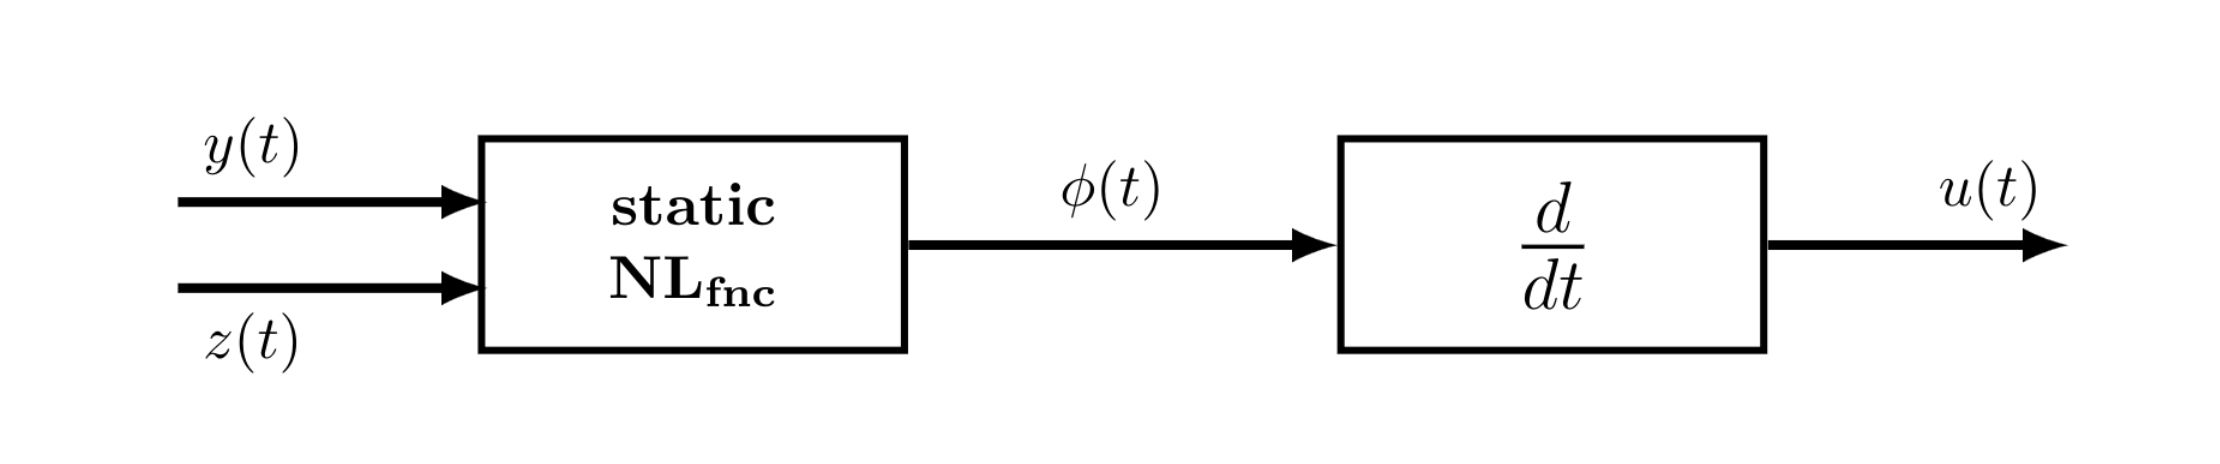
\includegraphics[width=8cm]{drawings/model.png}
    \caption{Блок-модель датчика}
    \label{fig:model}
\end{figure}

\section{Ход эксперимента}

Для выполнения экспреримента воспользуемся установкой из \cite{string-lab}. Из оборудование нам потребуется:

\begin{enumerate}
    \item Установка из \cite{string-lab} и генератор сигнала для возбуждения стоячик волн в струне \label{item:generator}
    \item Исследуемый Humbucker звукосниматель
    \item Вспомогательный датчик для регистрации движения струны \label{item:sensor}
    \item Цифровой осциллограф DS-1054Z \label{item:osc}
    \item Оптическая платформа с микрометричским винтом в вертикальной оси
    \item Изделия для крепления датчика к платформе, различные 3d-printed аксессуары
\end{enumerate}

Собранная установка представлена на \ref{fig:lab-setup}.
Возбуждая стоячую волну на главной частоте колебаний струны ($\approx 135$ Hz) получим колебания в пучности в центре струны.
Вспомогательный датчик \ref{item:sensor} расположим вблизи зафиксированного узла. Работаем в предположении линейного режима
колебаний. Все каналы осциллографа \ref{item:osc} настроены в закрытый режим $AC-coupling$. Земля всех каналов объединена внутри
осциллографа. Один из каналов использовался для объединения земли с металлической установкой (для уменьшения наведенных шумов).

\begin{figure}[h]
    \centering
    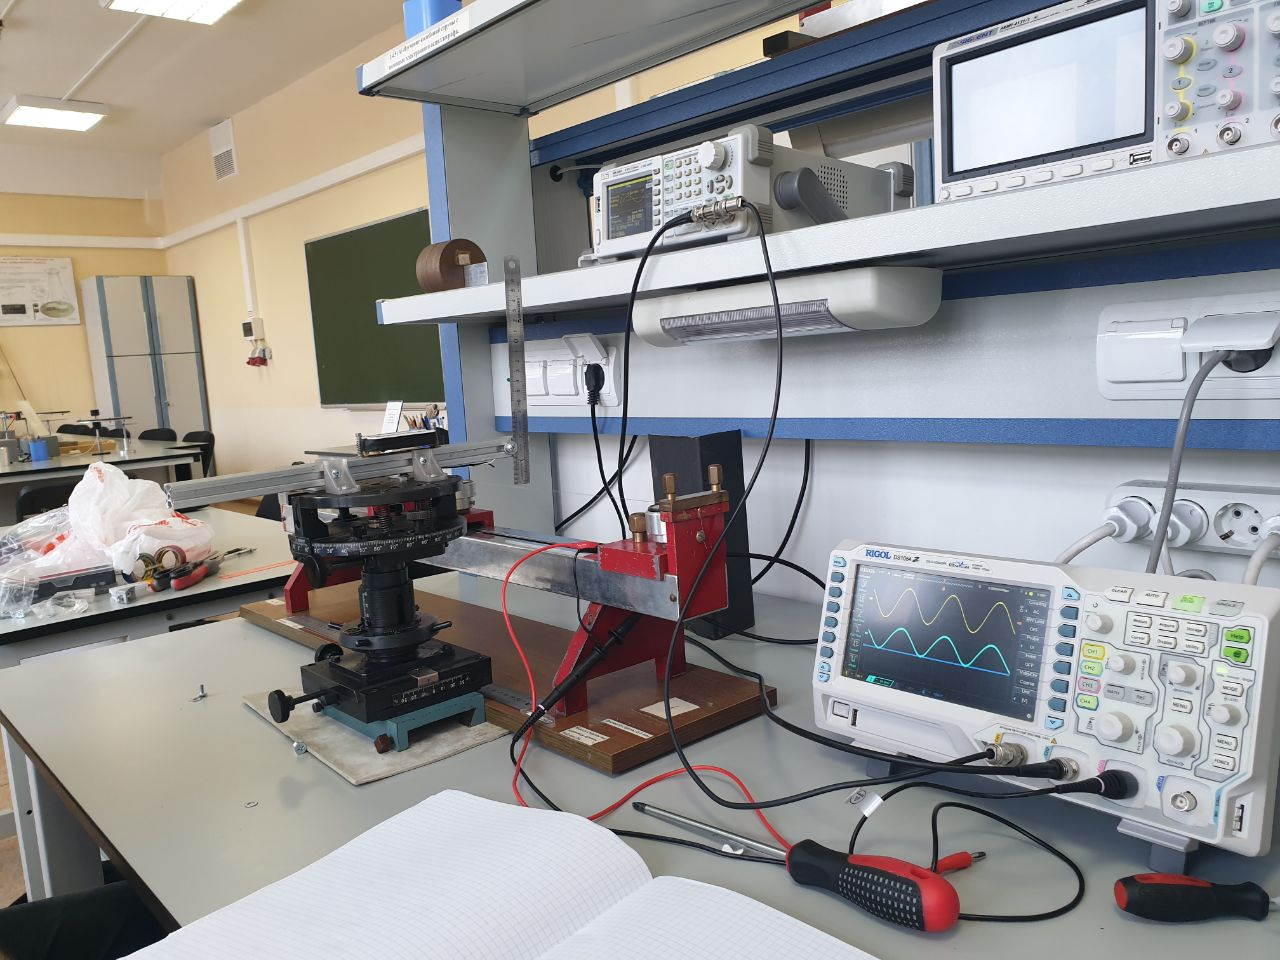
\includegraphics[width=8cm]{drawings/lab-setup.png}
    \caption{Экспериментальная установка}
    \label{fig:lab-setup}
\end{figure}

\subsection{Калибровка}

\begin{figure}[h]
    \centering
    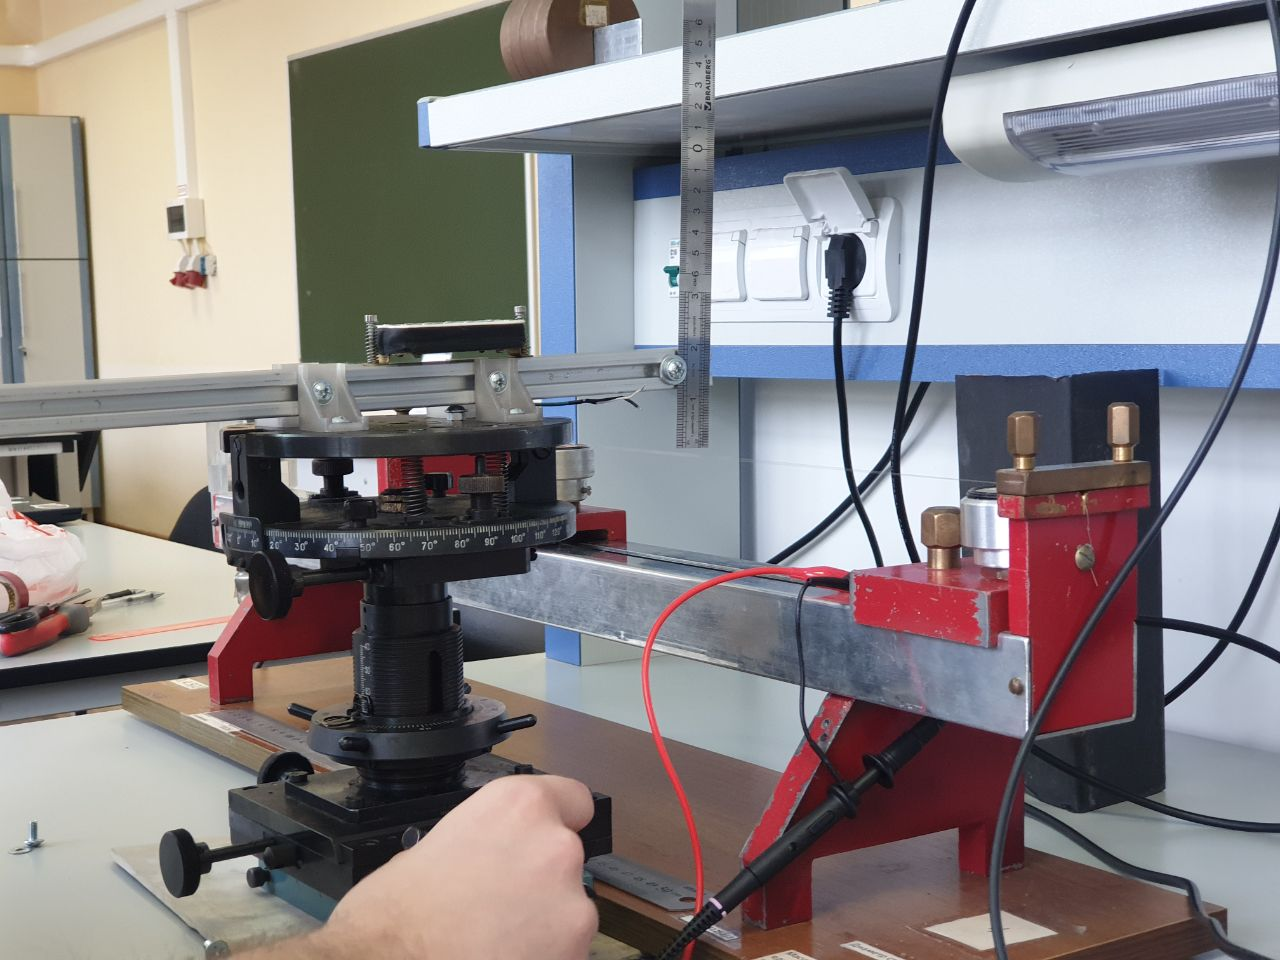
\includegraphics[width=8cm]{drawings/tuning.jpg}
		\caption{Процесс калибровки}
    \label{fig:lab-setup}
\end{figure}


Откалибруем зависимость амлитуды колебаний струны в пучности $z_{max}$ от амлитуды сигнала $v_{sensor}$, снимаемого с \ref{item:sensor}.
С помощью регулируемой платформы и острого объекта (металлической линейки) будем измерять $z_{max}/2$ постепенно приближая
конец линейки, пока не начнется \textit{дребезг}. Для набора напряжений генератора \ref{item:generator} проведем описанную процедуру
и зафиксируем данные с \ref{item:osc} и микрометрического винта. Нетрудно понять, что в линейном режиме колебаний струны следует ожидать
линейную зависимость $z_{max}(v_{sensor})$. Действительно, уравнение стоячей волны имеет вид:

\begin{equation}
    z(x, t) = z_{max} sin(k_n x) sin(\omega t)
\end{equation}

Где $k_n$ находится из условия $\lambda_n = \frac{2 L}{n}$ (в нашем эксперименте $n = 1$).
В пучности $z(t) = z_{max} sin(\omega t)$. Понятно, что $y'(t) = z_{max} \omega cos(\omega t)$, а напряжение $v_{sensor}$
на датчике \ref{item:sensor} определяется как:

\begin{equation}
    v_{sensor} = \frac{d \Phi}{dt} = \frac{d \Phi}{dz} \frac{dz}{dt} = \frac{d \Phi}{dz} y'(t)
\end{equation}

Так как сенсор \ref{item:sensor} располежен вблизи узла, то $\frac{d \Phi}{dz} \approx const$.

\begin{figure}[h]
    \centering
    %% Creator: Matplotlib, PGF backend
%%
%% To include the figure in your LaTeX document, write
%%   \input{<filename>.pgf}
%%
%% Make sure the required packages are loaded in your preamble
%%   \usepackage{pgf}
%%
%% Also ensure that all the required font packages are loaded; for instance,
%% the lmodern package is sometimes necessary when using math font.
%%   \usepackage{lmodern}
%%
%% Figures using additional raster images can only be included by \input if
%% they are in the same directory as the main LaTeX file. For loading figures
%% from other directories you can use the `import` package
%%   \usepackage{import}
%%
%% and then include the figures with
%%   \import{<path to file>}{<filename>.pgf}
%%
%% Matplotlib used the following preamble
%%   \def\mathdefault#1{#1}
%%   \everymath=\expandafter{\the\everymath\displaystyle}
%%   \usepackage{polyglossia}
%%   \usepackage{fontspec}
%%   \setmainfont{Liberation Serif}
%%   \setsansfont{Liberation Sans}
%%   \setmonofont{Liberation Mono}
%%   \usepackage{fontspec}
%%   \makeatletter\@ifpackageloaded{underscore}{}{\usepackage[strings]{underscore}}\makeatother
%%
\begingroup%
\makeatletter%
\begin{pgfpicture}%
\pgfpathrectangle{\pgfpointorigin}{\pgfqpoint{4.000000in}{3.000000in}}%
\pgfusepath{use as bounding box, clip}%
\begin{pgfscope}%
\pgfsetbuttcap%
\pgfsetmiterjoin%
\definecolor{currentfill}{rgb}{1.000000,1.000000,1.000000}%
\pgfsetfillcolor{currentfill}%
\pgfsetlinewidth{0.000000pt}%
\definecolor{currentstroke}{rgb}{1.000000,1.000000,1.000000}%
\pgfsetstrokecolor{currentstroke}%
\pgfsetdash{}{0pt}%
\pgfpathmoveto{\pgfqpoint{0.000000in}{0.000000in}}%
\pgfpathlineto{\pgfqpoint{4.000000in}{0.000000in}}%
\pgfpathlineto{\pgfqpoint{4.000000in}{3.000000in}}%
\pgfpathlineto{\pgfqpoint{0.000000in}{3.000000in}}%
\pgfpathlineto{\pgfqpoint{0.000000in}{0.000000in}}%
\pgfpathclose%
\pgfusepath{fill}%
\end{pgfscope}%
\begin{pgfscope}%
\pgfsetbuttcap%
\pgfsetmiterjoin%
\definecolor{currentfill}{rgb}{1.000000,1.000000,1.000000}%
\pgfsetfillcolor{currentfill}%
\pgfsetlinewidth{0.000000pt}%
\definecolor{currentstroke}{rgb}{0.000000,0.000000,0.000000}%
\pgfsetstrokecolor{currentstroke}%
\pgfsetstrokeopacity{0.000000}%
\pgfsetdash{}{0pt}%
\pgfpathmoveto{\pgfqpoint{0.606183in}{0.554649in}}%
\pgfpathlineto{\pgfqpoint{3.850000in}{0.554649in}}%
\pgfpathlineto{\pgfqpoint{3.850000in}{2.850000in}}%
\pgfpathlineto{\pgfqpoint{0.606183in}{2.850000in}}%
\pgfpathlineto{\pgfqpoint{0.606183in}{0.554649in}}%
\pgfpathclose%
\pgfusepath{fill}%
\end{pgfscope}%
\begin{pgfscope}%
\pgfpathrectangle{\pgfqpoint{0.606183in}{0.554649in}}{\pgfqpoint{3.243817in}{2.295351in}}%
\pgfusepath{clip}%
\pgfsetbuttcap%
\pgfsetroundjoin%
\definecolor{currentfill}{rgb}{1.000000,0.000000,0.000000}%
\pgfsetfillcolor{currentfill}%
\pgfsetlinewidth{1.505625pt}%
\definecolor{currentstroke}{rgb}{1.000000,0.000000,0.000000}%
\pgfsetstrokecolor{currentstroke}%
\pgfsetdash{}{0pt}%
\pgfsys@defobject{currentmarker}{\pgfqpoint{-0.041667in}{-0.041667in}}{\pgfqpoint{0.041667in}{0.041667in}}{%
\pgfpathmoveto{\pgfqpoint{-0.041667in}{-0.041667in}}%
\pgfpathlineto{\pgfqpoint{0.041667in}{0.041667in}}%
\pgfpathmoveto{\pgfqpoint{-0.041667in}{0.041667in}}%
\pgfpathlineto{\pgfqpoint{0.041667in}{-0.041667in}}%
\pgfusepath{stroke,fill}%
}%
\begin{pgfscope}%
\pgfsys@transformshift{2.228092in}{1.745651in}%
\pgfsys@useobject{currentmarker}{}%
\end{pgfscope}%
\begin{pgfscope}%
\pgfsys@transformshift{2.433623in}{1.835548in}%
\pgfsys@useobject{currentmarker}{}%
\end{pgfscope}%
\begin{pgfscope}%
\pgfsys@transformshift{2.013624in}{1.565855in}%
\pgfsys@useobject{currentmarker}{}%
\end{pgfscope}%
\begin{pgfscope}%
\pgfsys@transformshift{1.432776in}{1.071417in}%
\pgfsys@useobject{currentmarker}{}%
\end{pgfscope}%
\begin{pgfscope}%
\pgfsys@transformshift{2.960855in}{2.195140in}%
\pgfsys@useobject{currentmarker}{}%
\end{pgfscope}%
\begin{pgfscope}%
\pgfsys@transformshift{3.032344in}{2.419884in}%
\pgfsys@useobject{currentmarker}{}%
\end{pgfscope}%
\begin{pgfscope}%
\pgfsys@transformshift{3.702554in}{2.644629in}%
\pgfsys@useobject{currentmarker}{}%
\end{pgfscope}%
\end{pgfscope}%
\begin{pgfscope}%
\pgfpathrectangle{\pgfqpoint{0.606183in}{0.554649in}}{\pgfqpoint{3.243817in}{2.295351in}}%
\pgfusepath{clip}%
\pgfsetrectcap%
\pgfsetroundjoin%
\pgfsetlinewidth{0.803000pt}%
\definecolor{currentstroke}{rgb}{0.690196,0.690196,0.690196}%
\pgfsetstrokecolor{currentstroke}%
\pgfsetdash{}{0pt}%
\pgfpathmoveto{\pgfqpoint{0.753630in}{0.554649in}}%
\pgfpathlineto{\pgfqpoint{0.753630in}{2.850000in}}%
\pgfusepath{stroke}%
\end{pgfscope}%
\begin{pgfscope}%
\pgfsetbuttcap%
\pgfsetroundjoin%
\definecolor{currentfill}{rgb}{0.000000,0.000000,0.000000}%
\pgfsetfillcolor{currentfill}%
\pgfsetlinewidth{0.803000pt}%
\definecolor{currentstroke}{rgb}{0.000000,0.000000,0.000000}%
\pgfsetstrokecolor{currentstroke}%
\pgfsetdash{}{0pt}%
\pgfsys@defobject{currentmarker}{\pgfqpoint{0.000000in}{-0.048611in}}{\pgfqpoint{0.000000in}{0.000000in}}{%
\pgfpathmoveto{\pgfqpoint{0.000000in}{0.000000in}}%
\pgfpathlineto{\pgfqpoint{0.000000in}{-0.048611in}}%
\pgfusepath{stroke,fill}%
}%
\begin{pgfscope}%
\pgfsys@transformshift{0.753630in}{0.554649in}%
\pgfsys@useobject{currentmarker}{}%
\end{pgfscope}%
\end{pgfscope}%
\begin{pgfscope}%
\definecolor{textcolor}{rgb}{0.000000,0.000000,0.000000}%
\pgfsetstrokecolor{textcolor}%
\pgfsetfillcolor{textcolor}%
\pgftext[x=0.753630in,y=0.457427in,,top]{\color{textcolor}{\rmfamily\fontsize{10.000000}{12.000000}\selectfont\catcode`\^=\active\def^{\ifmmode\sp\else\^{}\fi}\catcode`\%=\active\def%{\%}$\mathdefault{0}$}}%
\end{pgfscope}%
\begin{pgfscope}%
\pgfpathrectangle{\pgfqpoint{0.606183in}{0.554649in}}{\pgfqpoint{3.243817in}{2.295351in}}%
\pgfusepath{clip}%
\pgfsetrectcap%
\pgfsetroundjoin%
\pgfsetlinewidth{0.803000pt}%
\definecolor{currentstroke}{rgb}{0.690196,0.690196,0.690196}%
\pgfsetstrokecolor{currentstroke}%
\pgfsetdash{}{0pt}%
\pgfpathmoveto{\pgfqpoint{1.647243in}{0.554649in}}%
\pgfpathlineto{\pgfqpoint{1.647243in}{2.850000in}}%
\pgfusepath{stroke}%
\end{pgfscope}%
\begin{pgfscope}%
\pgfsetbuttcap%
\pgfsetroundjoin%
\definecolor{currentfill}{rgb}{0.000000,0.000000,0.000000}%
\pgfsetfillcolor{currentfill}%
\pgfsetlinewidth{0.803000pt}%
\definecolor{currentstroke}{rgb}{0.000000,0.000000,0.000000}%
\pgfsetstrokecolor{currentstroke}%
\pgfsetdash{}{0pt}%
\pgfsys@defobject{currentmarker}{\pgfqpoint{0.000000in}{-0.048611in}}{\pgfqpoint{0.000000in}{0.000000in}}{%
\pgfpathmoveto{\pgfqpoint{0.000000in}{0.000000in}}%
\pgfpathlineto{\pgfqpoint{0.000000in}{-0.048611in}}%
\pgfusepath{stroke,fill}%
}%
\begin{pgfscope}%
\pgfsys@transformshift{1.647243in}{0.554649in}%
\pgfsys@useobject{currentmarker}{}%
\end{pgfscope}%
\end{pgfscope}%
\begin{pgfscope}%
\definecolor{textcolor}{rgb}{0.000000,0.000000,0.000000}%
\pgfsetstrokecolor{textcolor}%
\pgfsetfillcolor{textcolor}%
\pgftext[x=1.647243in,y=0.457427in,,top]{\color{textcolor}{\rmfamily\fontsize{10.000000}{12.000000}\selectfont\catcode`\^=\active\def^{\ifmmode\sp\else\^{}\fi}\catcode`\%=\active\def%{\%}$\mathdefault{20}$}}%
\end{pgfscope}%
\begin{pgfscope}%
\pgfpathrectangle{\pgfqpoint{0.606183in}{0.554649in}}{\pgfqpoint{3.243817in}{2.295351in}}%
\pgfusepath{clip}%
\pgfsetrectcap%
\pgfsetroundjoin%
\pgfsetlinewidth{0.803000pt}%
\definecolor{currentstroke}{rgb}{0.690196,0.690196,0.690196}%
\pgfsetstrokecolor{currentstroke}%
\pgfsetdash{}{0pt}%
\pgfpathmoveto{\pgfqpoint{2.540856in}{0.554649in}}%
\pgfpathlineto{\pgfqpoint{2.540856in}{2.850000in}}%
\pgfusepath{stroke}%
\end{pgfscope}%
\begin{pgfscope}%
\pgfsetbuttcap%
\pgfsetroundjoin%
\definecolor{currentfill}{rgb}{0.000000,0.000000,0.000000}%
\pgfsetfillcolor{currentfill}%
\pgfsetlinewidth{0.803000pt}%
\definecolor{currentstroke}{rgb}{0.000000,0.000000,0.000000}%
\pgfsetstrokecolor{currentstroke}%
\pgfsetdash{}{0pt}%
\pgfsys@defobject{currentmarker}{\pgfqpoint{0.000000in}{-0.048611in}}{\pgfqpoint{0.000000in}{0.000000in}}{%
\pgfpathmoveto{\pgfqpoint{0.000000in}{0.000000in}}%
\pgfpathlineto{\pgfqpoint{0.000000in}{-0.048611in}}%
\pgfusepath{stroke,fill}%
}%
\begin{pgfscope}%
\pgfsys@transformshift{2.540856in}{0.554649in}%
\pgfsys@useobject{currentmarker}{}%
\end{pgfscope}%
\end{pgfscope}%
\begin{pgfscope}%
\definecolor{textcolor}{rgb}{0.000000,0.000000,0.000000}%
\pgfsetstrokecolor{textcolor}%
\pgfsetfillcolor{textcolor}%
\pgftext[x=2.540856in,y=0.457427in,,top]{\color{textcolor}{\rmfamily\fontsize{10.000000}{12.000000}\selectfont\catcode`\^=\active\def^{\ifmmode\sp\else\^{}\fi}\catcode`\%=\active\def%{\%}$\mathdefault{40}$}}%
\end{pgfscope}%
\begin{pgfscope}%
\pgfpathrectangle{\pgfqpoint{0.606183in}{0.554649in}}{\pgfqpoint{3.243817in}{2.295351in}}%
\pgfusepath{clip}%
\pgfsetrectcap%
\pgfsetroundjoin%
\pgfsetlinewidth{0.803000pt}%
\definecolor{currentstroke}{rgb}{0.690196,0.690196,0.690196}%
\pgfsetstrokecolor{currentstroke}%
\pgfsetdash{}{0pt}%
\pgfpathmoveto{\pgfqpoint{3.434470in}{0.554649in}}%
\pgfpathlineto{\pgfqpoint{3.434470in}{2.850000in}}%
\pgfusepath{stroke}%
\end{pgfscope}%
\begin{pgfscope}%
\pgfsetbuttcap%
\pgfsetroundjoin%
\definecolor{currentfill}{rgb}{0.000000,0.000000,0.000000}%
\pgfsetfillcolor{currentfill}%
\pgfsetlinewidth{0.803000pt}%
\definecolor{currentstroke}{rgb}{0.000000,0.000000,0.000000}%
\pgfsetstrokecolor{currentstroke}%
\pgfsetdash{}{0pt}%
\pgfsys@defobject{currentmarker}{\pgfqpoint{0.000000in}{-0.048611in}}{\pgfqpoint{0.000000in}{0.000000in}}{%
\pgfpathmoveto{\pgfqpoint{0.000000in}{0.000000in}}%
\pgfpathlineto{\pgfqpoint{0.000000in}{-0.048611in}}%
\pgfusepath{stroke,fill}%
}%
\begin{pgfscope}%
\pgfsys@transformshift{3.434470in}{0.554649in}%
\pgfsys@useobject{currentmarker}{}%
\end{pgfscope}%
\end{pgfscope}%
\begin{pgfscope}%
\definecolor{textcolor}{rgb}{0.000000,0.000000,0.000000}%
\pgfsetstrokecolor{textcolor}%
\pgfsetfillcolor{textcolor}%
\pgftext[x=3.434470in,y=0.457427in,,top]{\color{textcolor}{\rmfamily\fontsize{10.000000}{12.000000}\selectfont\catcode`\^=\active\def^{\ifmmode\sp\else\^{}\fi}\catcode`\%=\active\def%{\%}$\mathdefault{60}$}}%
\end{pgfscope}%
\begin{pgfscope}%
\definecolor{textcolor}{rgb}{0.000000,0.000000,0.000000}%
\pgfsetstrokecolor{textcolor}%
\pgfsetfillcolor{textcolor}%
\pgftext[x=2.228092in,y=0.275936in,,top]{\color{textcolor}{\rmfamily\fontsize{10.000000}{12.000000}\selectfont\catcode`\^=\active\def^{\ifmmode\sp\else\^{}\fi}\catcode`\%=\active\def%{\%}$v_{max}$, мВ}}%
\end{pgfscope}%
\begin{pgfscope}%
\pgfpathrectangle{\pgfqpoint{0.606183in}{0.554649in}}{\pgfqpoint{3.243817in}{2.295351in}}%
\pgfusepath{clip}%
\pgfsetrectcap%
\pgfsetroundjoin%
\pgfsetlinewidth{0.803000pt}%
\definecolor{currentstroke}{rgb}{0.690196,0.690196,0.690196}%
\pgfsetstrokecolor{currentstroke}%
\pgfsetdash{}{0pt}%
\pgfpathmoveto{\pgfqpoint{0.606183in}{1.003994in}}%
\pgfpathlineto{\pgfqpoint{3.850000in}{1.003994in}}%
\pgfusepath{stroke}%
\end{pgfscope}%
\begin{pgfscope}%
\pgfsetbuttcap%
\pgfsetroundjoin%
\definecolor{currentfill}{rgb}{0.000000,0.000000,0.000000}%
\pgfsetfillcolor{currentfill}%
\pgfsetlinewidth{0.803000pt}%
\definecolor{currentstroke}{rgb}{0.000000,0.000000,0.000000}%
\pgfsetstrokecolor{currentstroke}%
\pgfsetdash{}{0pt}%
\pgfsys@defobject{currentmarker}{\pgfqpoint{-0.048611in}{0.000000in}}{\pgfqpoint{-0.000000in}{0.000000in}}{%
\pgfpathmoveto{\pgfqpoint{-0.000000in}{0.000000in}}%
\pgfpathlineto{\pgfqpoint{-0.048611in}{0.000000in}}%
\pgfusepath{stroke,fill}%
}%
\begin{pgfscope}%
\pgfsys@transformshift{0.606183in}{1.003994in}%
\pgfsys@useobject{currentmarker}{}%
\end{pgfscope}%
\end{pgfscope}%
\begin{pgfscope}%
\definecolor{textcolor}{rgb}{0.000000,0.000000,0.000000}%
\pgfsetstrokecolor{textcolor}%
\pgfsetfillcolor{textcolor}%
\pgftext[x=0.331491in, y=0.955810in, left, base]{\color{textcolor}{\rmfamily\fontsize{10.000000}{12.000000}\selectfont\catcode`\^=\active\def^{\ifmmode\sp\else\^{}\fi}\catcode`\%=\active\def%{\%}$\mathdefault{0.1}$}}%
\end{pgfscope}%
\begin{pgfscope}%
\pgfpathrectangle{\pgfqpoint{0.606183in}{0.554649in}}{\pgfqpoint{3.243817in}{2.295351in}}%
\pgfusepath{clip}%
\pgfsetrectcap%
\pgfsetroundjoin%
\pgfsetlinewidth{0.803000pt}%
\definecolor{currentstroke}{rgb}{0.690196,0.690196,0.690196}%
\pgfsetstrokecolor{currentstroke}%
\pgfsetdash{}{0pt}%
\pgfpathmoveto{\pgfqpoint{0.606183in}{1.453483in}}%
\pgfpathlineto{\pgfqpoint{3.850000in}{1.453483in}}%
\pgfusepath{stroke}%
\end{pgfscope}%
\begin{pgfscope}%
\pgfsetbuttcap%
\pgfsetroundjoin%
\definecolor{currentfill}{rgb}{0.000000,0.000000,0.000000}%
\pgfsetfillcolor{currentfill}%
\pgfsetlinewidth{0.803000pt}%
\definecolor{currentstroke}{rgb}{0.000000,0.000000,0.000000}%
\pgfsetstrokecolor{currentstroke}%
\pgfsetdash{}{0pt}%
\pgfsys@defobject{currentmarker}{\pgfqpoint{-0.048611in}{0.000000in}}{\pgfqpoint{-0.000000in}{0.000000in}}{%
\pgfpathmoveto{\pgfqpoint{-0.000000in}{0.000000in}}%
\pgfpathlineto{\pgfqpoint{-0.048611in}{0.000000in}}%
\pgfusepath{stroke,fill}%
}%
\begin{pgfscope}%
\pgfsys@transformshift{0.606183in}{1.453483in}%
\pgfsys@useobject{currentmarker}{}%
\end{pgfscope}%
\end{pgfscope}%
\begin{pgfscope}%
\definecolor{textcolor}{rgb}{0.000000,0.000000,0.000000}%
\pgfsetstrokecolor{textcolor}%
\pgfsetfillcolor{textcolor}%
\pgftext[x=0.331491in, y=1.405299in, left, base]{\color{textcolor}{\rmfamily\fontsize{10.000000}{12.000000}\selectfont\catcode`\^=\active\def^{\ifmmode\sp\else\^{}\fi}\catcode`\%=\active\def%{\%}$\mathdefault{0.2}$}}%
\end{pgfscope}%
\begin{pgfscope}%
\pgfpathrectangle{\pgfqpoint{0.606183in}{0.554649in}}{\pgfqpoint{3.243817in}{2.295351in}}%
\pgfusepath{clip}%
\pgfsetrectcap%
\pgfsetroundjoin%
\pgfsetlinewidth{0.803000pt}%
\definecolor{currentstroke}{rgb}{0.690196,0.690196,0.690196}%
\pgfsetstrokecolor{currentstroke}%
\pgfsetdash{}{0pt}%
\pgfpathmoveto{\pgfqpoint{0.606183in}{1.902972in}}%
\pgfpathlineto{\pgfqpoint{3.850000in}{1.902972in}}%
\pgfusepath{stroke}%
\end{pgfscope}%
\begin{pgfscope}%
\pgfsetbuttcap%
\pgfsetroundjoin%
\definecolor{currentfill}{rgb}{0.000000,0.000000,0.000000}%
\pgfsetfillcolor{currentfill}%
\pgfsetlinewidth{0.803000pt}%
\definecolor{currentstroke}{rgb}{0.000000,0.000000,0.000000}%
\pgfsetstrokecolor{currentstroke}%
\pgfsetdash{}{0pt}%
\pgfsys@defobject{currentmarker}{\pgfqpoint{-0.048611in}{0.000000in}}{\pgfqpoint{-0.000000in}{0.000000in}}{%
\pgfpathmoveto{\pgfqpoint{-0.000000in}{0.000000in}}%
\pgfpathlineto{\pgfqpoint{-0.048611in}{0.000000in}}%
\pgfusepath{stroke,fill}%
}%
\begin{pgfscope}%
\pgfsys@transformshift{0.606183in}{1.902972in}%
\pgfsys@useobject{currentmarker}{}%
\end{pgfscope}%
\end{pgfscope}%
\begin{pgfscope}%
\definecolor{textcolor}{rgb}{0.000000,0.000000,0.000000}%
\pgfsetstrokecolor{textcolor}%
\pgfsetfillcolor{textcolor}%
\pgftext[x=0.331491in, y=1.854788in, left, base]{\color{textcolor}{\rmfamily\fontsize{10.000000}{12.000000}\selectfont\catcode`\^=\active\def^{\ifmmode\sp\else\^{}\fi}\catcode`\%=\active\def%{\%}$\mathdefault{0.3}$}}%
\end{pgfscope}%
\begin{pgfscope}%
\pgfpathrectangle{\pgfqpoint{0.606183in}{0.554649in}}{\pgfqpoint{3.243817in}{2.295351in}}%
\pgfusepath{clip}%
\pgfsetrectcap%
\pgfsetroundjoin%
\pgfsetlinewidth{0.803000pt}%
\definecolor{currentstroke}{rgb}{0.690196,0.690196,0.690196}%
\pgfsetstrokecolor{currentstroke}%
\pgfsetdash{}{0pt}%
\pgfpathmoveto{\pgfqpoint{0.606183in}{2.352461in}}%
\pgfpathlineto{\pgfqpoint{3.850000in}{2.352461in}}%
\pgfusepath{stroke}%
\end{pgfscope}%
\begin{pgfscope}%
\pgfsetbuttcap%
\pgfsetroundjoin%
\definecolor{currentfill}{rgb}{0.000000,0.000000,0.000000}%
\pgfsetfillcolor{currentfill}%
\pgfsetlinewidth{0.803000pt}%
\definecolor{currentstroke}{rgb}{0.000000,0.000000,0.000000}%
\pgfsetstrokecolor{currentstroke}%
\pgfsetdash{}{0pt}%
\pgfsys@defobject{currentmarker}{\pgfqpoint{-0.048611in}{0.000000in}}{\pgfqpoint{-0.000000in}{0.000000in}}{%
\pgfpathmoveto{\pgfqpoint{-0.000000in}{0.000000in}}%
\pgfpathlineto{\pgfqpoint{-0.048611in}{0.000000in}}%
\pgfusepath{stroke,fill}%
}%
\begin{pgfscope}%
\pgfsys@transformshift{0.606183in}{2.352461in}%
\pgfsys@useobject{currentmarker}{}%
\end{pgfscope}%
\end{pgfscope}%
\begin{pgfscope}%
\definecolor{textcolor}{rgb}{0.000000,0.000000,0.000000}%
\pgfsetstrokecolor{textcolor}%
\pgfsetfillcolor{textcolor}%
\pgftext[x=0.331491in, y=2.304277in, left, base]{\color{textcolor}{\rmfamily\fontsize{10.000000}{12.000000}\selectfont\catcode`\^=\active\def^{\ifmmode\sp\else\^{}\fi}\catcode`\%=\active\def%{\%}$\mathdefault{0.4}$}}%
\end{pgfscope}%
\begin{pgfscope}%
\pgfpathrectangle{\pgfqpoint{0.606183in}{0.554649in}}{\pgfqpoint{3.243817in}{2.295351in}}%
\pgfusepath{clip}%
\pgfsetrectcap%
\pgfsetroundjoin%
\pgfsetlinewidth{0.803000pt}%
\definecolor{currentstroke}{rgb}{0.690196,0.690196,0.690196}%
\pgfsetstrokecolor{currentstroke}%
\pgfsetdash{}{0pt}%
\pgfpathmoveto{\pgfqpoint{0.606183in}{2.801950in}}%
\pgfpathlineto{\pgfqpoint{3.850000in}{2.801950in}}%
\pgfusepath{stroke}%
\end{pgfscope}%
\begin{pgfscope}%
\pgfsetbuttcap%
\pgfsetroundjoin%
\definecolor{currentfill}{rgb}{0.000000,0.000000,0.000000}%
\pgfsetfillcolor{currentfill}%
\pgfsetlinewidth{0.803000pt}%
\definecolor{currentstroke}{rgb}{0.000000,0.000000,0.000000}%
\pgfsetstrokecolor{currentstroke}%
\pgfsetdash{}{0pt}%
\pgfsys@defobject{currentmarker}{\pgfqpoint{-0.048611in}{0.000000in}}{\pgfqpoint{-0.000000in}{0.000000in}}{%
\pgfpathmoveto{\pgfqpoint{-0.000000in}{0.000000in}}%
\pgfpathlineto{\pgfqpoint{-0.048611in}{0.000000in}}%
\pgfusepath{stroke,fill}%
}%
\begin{pgfscope}%
\pgfsys@transformshift{0.606183in}{2.801950in}%
\pgfsys@useobject{currentmarker}{}%
\end{pgfscope}%
\end{pgfscope}%
\begin{pgfscope}%
\definecolor{textcolor}{rgb}{0.000000,0.000000,0.000000}%
\pgfsetstrokecolor{textcolor}%
\pgfsetfillcolor{textcolor}%
\pgftext[x=0.331491in, y=2.753766in, left, base]{\color{textcolor}{\rmfamily\fontsize{10.000000}{12.000000}\selectfont\catcode`\^=\active\def^{\ifmmode\sp\else\^{}\fi}\catcode`\%=\active\def%{\%}$\mathdefault{0.5}$}}%
\end{pgfscope}%
\begin{pgfscope}%
\definecolor{textcolor}{rgb}{0.000000,0.000000,0.000000}%
\pgfsetstrokecolor{textcolor}%
\pgfsetfillcolor{textcolor}%
\pgftext[x=0.275936in,y=1.702325in,,bottom,rotate=90.000000]{\color{textcolor}{\rmfamily\fontsize{10.000000}{12.000000}\selectfont\catcode`\^=\active\def^{\ifmmode\sp\else\^{}\fi}\catcode`\%=\active\def%{\%}$\Delta{z}$, мм}}%
\end{pgfscope}%
\begin{pgfscope}%
\pgfpathrectangle{\pgfqpoint{0.606183in}{0.554649in}}{\pgfqpoint{3.243817in}{2.295351in}}%
\pgfusepath{clip}%
\pgfsetrectcap%
\pgfsetroundjoin%
\pgfsetlinewidth{1.505625pt}%
\definecolor{currentstroke}{rgb}{0.121569,0.466667,0.705882}%
\pgfsetstrokecolor{currentstroke}%
\pgfsetdash{}{0pt}%
\pgfpathmoveto{\pgfqpoint{0.753630in}{0.658984in}}%
\pgfpathlineto{\pgfqpoint{3.702554in}{2.745666in}}%
\pgfusepath{stroke}%
\end{pgfscope}%
\begin{pgfscope}%
\pgfsetrectcap%
\pgfsetmiterjoin%
\pgfsetlinewidth{0.803000pt}%
\definecolor{currentstroke}{rgb}{0.000000,0.000000,0.000000}%
\pgfsetstrokecolor{currentstroke}%
\pgfsetdash{}{0pt}%
\pgfpathmoveto{\pgfqpoint{0.606183in}{0.554649in}}%
\pgfpathlineto{\pgfqpoint{0.606183in}{2.850000in}}%
\pgfusepath{stroke}%
\end{pgfscope}%
\begin{pgfscope}%
\pgfsetrectcap%
\pgfsetmiterjoin%
\pgfsetlinewidth{0.803000pt}%
\definecolor{currentstroke}{rgb}{0.000000,0.000000,0.000000}%
\pgfsetstrokecolor{currentstroke}%
\pgfsetdash{}{0pt}%
\pgfpathmoveto{\pgfqpoint{3.850000in}{0.554649in}}%
\pgfpathlineto{\pgfqpoint{3.850000in}{2.850000in}}%
\pgfusepath{stroke}%
\end{pgfscope}%
\begin{pgfscope}%
\pgfsetrectcap%
\pgfsetmiterjoin%
\pgfsetlinewidth{0.803000pt}%
\definecolor{currentstroke}{rgb}{0.000000,0.000000,0.000000}%
\pgfsetstrokecolor{currentstroke}%
\pgfsetdash{}{0pt}%
\pgfpathmoveto{\pgfqpoint{0.606183in}{0.554649in}}%
\pgfpathlineto{\pgfqpoint{3.850000in}{0.554649in}}%
\pgfusepath{stroke}%
\end{pgfscope}%
\begin{pgfscope}%
\pgfsetrectcap%
\pgfsetmiterjoin%
\pgfsetlinewidth{0.803000pt}%
\definecolor{currentstroke}{rgb}{0.000000,0.000000,0.000000}%
\pgfsetstrokecolor{currentstroke}%
\pgfsetdash{}{0pt}%
\pgfpathmoveto{\pgfqpoint{0.606183in}{2.850000in}}%
\pgfpathlineto{\pgfqpoint{3.850000in}{2.850000in}}%
\pgfusepath{stroke}%
\end{pgfscope}%
\end{pgfpicture}%
\makeatother%
\endgroup%

    \caption{Калибровочная зависимость $z_{max}(v_{sensor})$}
    \label{fig:model}
\end{figure}

Используя полученную калибровочную прямую мы можем косвенно измерять положение струны,
снимая показания с датчика.

\subsection{Измерение NL}

\begin{figure}[h]
    \centering
    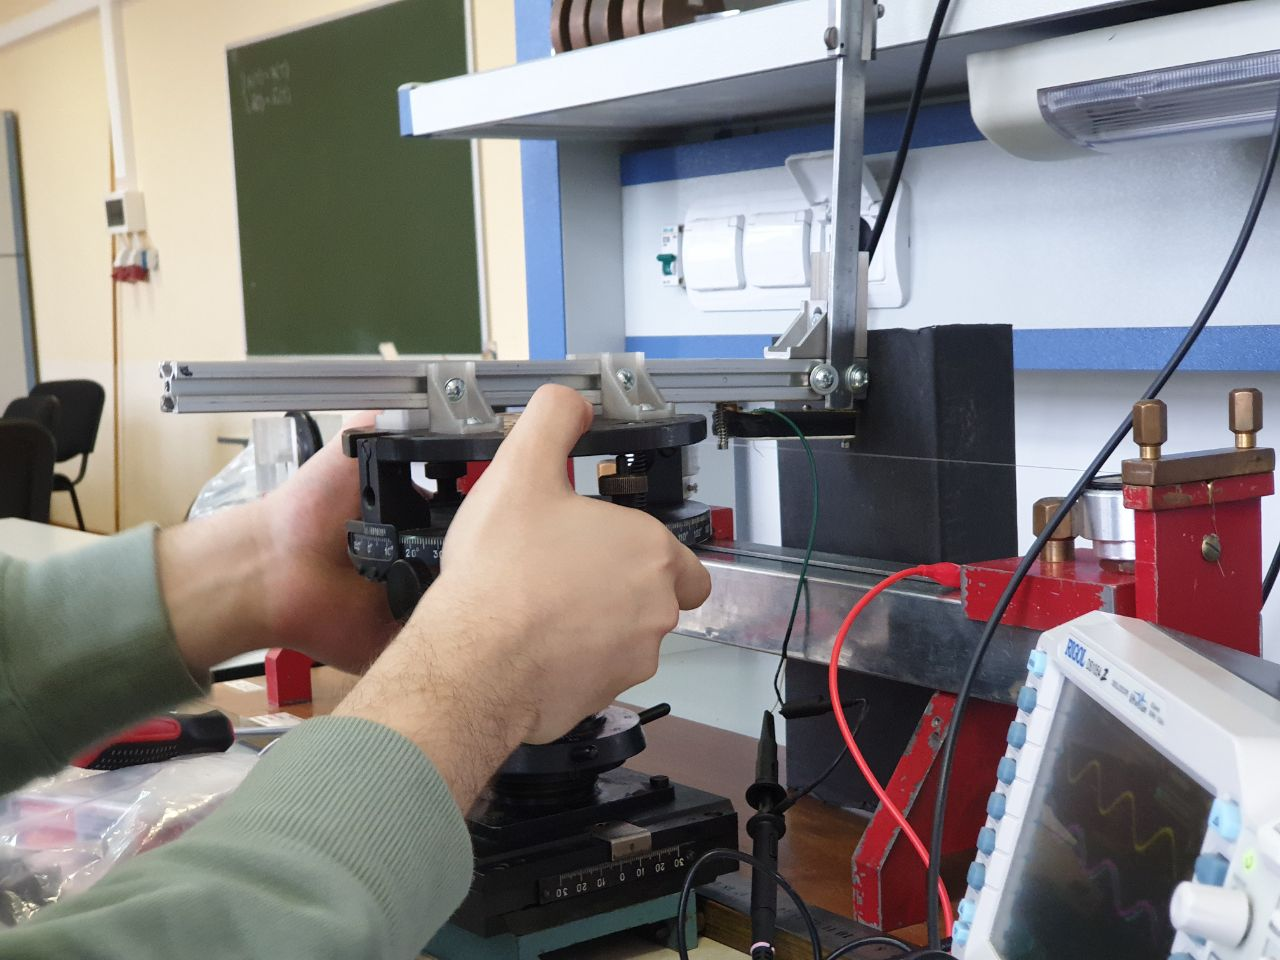
\includegraphics[width=8cm]{drawings/measurement.jpeg}
		\caption{Процесс основного измерения}
    \label{fig:lab-setup}
\end{figure}


Для измерения статической функции нелинейности (т.е. зависимость потока) от координаты $z$
воспользуемся методом, предложенным \cite{novak:hal-02512148}. При различных удалениях $z_0$ звукоснимателя от струны,
будем снимать с него значение напряжение $u(t)$. Вместе с этим, также снимая показания с датчика \ref{item:sensor} и имея
калибровочную зависимость получаем косвенное измерение положения струны в окрестности $z_0$. Измененяя $z_0$ инкрементами
$\approx 0.6$ мм можно замести интересуемый диапазон координат $z$. 
Интеграл напряжения $u(t)$ есть искомая функция $NL$, но как
зависимость от времени. Чтобы перейти к $NL(z)$ достаточно построить параметрический график $z = z(t)$, $NL = NL(t)$.

Для каждого положения звукоснимателя необходимо подстраивать частоту генератора, так как наличие магнитного поля звукоснимателя
влияет на резонансную частоту системы. Учитывая низкую добротность колебательной системы и чувствительностью к окружающим воздействиям,
измерение значительного интервала $z$ оказывается трудоемкой задачей.

Стоит учитвать, что на графике представлены координаты $z$ относительно некоторого начального положения оптической платформы,
а не расстояние до поверхности звукоснимателя. 

Предварительно, при обработке сигнала необходимо отфильтровать сигнал, снятый со звукоснимателя. Зависимость приведена на
рис. \ref{fig:spectrum}.

\begin{figure}
    \centering
    %% Creator: Matplotlib, PGF backend
%%
%% To include the figure in your LaTeX document, write
%%   \input{<filename>.pgf}
%%
%% Make sure the required packages are loaded in your preamble
%%   \usepackage{pgf}
%%
%% Also ensure that all the required font packages are loaded; for instance,
%% the lmodern package is sometimes necessary when using math font.
%%   \usepackage{lmodern}
%%
%% Figures using additional raster images can only be included by \input if
%% they are in the same directory as the main LaTeX file. For loading figures
%% from other directories you can use the `import` package
%%   \usepackage{import}
%%
%% and then include the figures with
%%   \import{<path to file>}{<filename>.pgf}
%%
%% Matplotlib used the following preamble
%%   \def\mathdefault#1{#1}
%%   \everymath=\expandafter{\the\everymath\displaystyle}
%%   \usepackage{polyglossia}
%%   \usepackage{fontspec}
%%   \setmainfont{Liberation Serif}
%%   \setsansfont{Liberation Sans}
%%   \setmonofont{Liberation Mono}
%%   \usepackage{fontspec}
%%   \makeatletter\@ifpackageloaded{underscore}{}{\usepackage[strings]{underscore}}\makeatother
%%
\begingroup%
\makeatletter%
\begin{pgfpicture}%
\pgfpathrectangle{\pgfpointorigin}{\pgfqpoint{5.000000in}{3.500000in}}%
\pgfusepath{use as bounding box, clip}%
\begin{pgfscope}%
\pgfsetbuttcap%
\pgfsetmiterjoin%
\definecolor{currentfill}{rgb}{1.000000,1.000000,1.000000}%
\pgfsetfillcolor{currentfill}%
\pgfsetlinewidth{0.000000pt}%
\definecolor{currentstroke}{rgb}{1.000000,1.000000,1.000000}%
\pgfsetstrokecolor{currentstroke}%
\pgfsetdash{}{0pt}%
\pgfpathmoveto{\pgfqpoint{0.000000in}{0.000000in}}%
\pgfpathlineto{\pgfqpoint{5.000000in}{0.000000in}}%
\pgfpathlineto{\pgfqpoint{5.000000in}{3.500000in}}%
\pgfpathlineto{\pgfqpoint{0.000000in}{3.500000in}}%
\pgfpathlineto{\pgfqpoint{0.000000in}{0.000000in}}%
\pgfpathclose%
\pgfusepath{fill}%
\end{pgfscope}%
\begin{pgfscope}%
\pgfsetbuttcap%
\pgfsetmiterjoin%
\definecolor{currentfill}{rgb}{1.000000,1.000000,1.000000}%
\pgfsetfillcolor{currentfill}%
\pgfsetlinewidth{0.000000pt}%
\definecolor{currentstroke}{rgb}{0.000000,0.000000,0.000000}%
\pgfsetstrokecolor{currentstroke}%
\pgfsetstrokeopacity{0.000000}%
\pgfsetdash{}{0pt}%
\pgfpathmoveto{\pgfqpoint{0.737636in}{0.554649in}}%
\pgfpathlineto{\pgfqpoint{4.676388in}{0.554649in}}%
\pgfpathlineto{\pgfqpoint{4.676388in}{3.151025in}}%
\pgfpathlineto{\pgfqpoint{0.737636in}{3.151025in}}%
\pgfpathlineto{\pgfqpoint{0.737636in}{0.554649in}}%
\pgfpathclose%
\pgfusepath{fill}%
\end{pgfscope}%
\begin{pgfscope}%
\pgfpathrectangle{\pgfqpoint{0.737636in}{0.554649in}}{\pgfqpoint{3.938752in}{2.596376in}}%
\pgfusepath{clip}%
\pgfsetrectcap%
\pgfsetroundjoin%
\pgfsetlinewidth{0.803000pt}%
\definecolor{currentstroke}{rgb}{0.690196,0.690196,0.690196}%
\pgfsetstrokecolor{currentstroke}%
\pgfsetdash{}{0pt}%
\pgfpathmoveto{\pgfqpoint{0.737636in}{0.554649in}}%
\pgfpathlineto{\pgfqpoint{0.737636in}{3.151025in}}%
\pgfusepath{stroke}%
\end{pgfscope}%
\begin{pgfscope}%
\pgfsetbuttcap%
\pgfsetroundjoin%
\definecolor{currentfill}{rgb}{0.000000,0.000000,0.000000}%
\pgfsetfillcolor{currentfill}%
\pgfsetlinewidth{0.803000pt}%
\definecolor{currentstroke}{rgb}{0.000000,0.000000,0.000000}%
\pgfsetstrokecolor{currentstroke}%
\pgfsetdash{}{0pt}%
\pgfsys@defobject{currentmarker}{\pgfqpoint{0.000000in}{-0.048611in}}{\pgfqpoint{0.000000in}{0.000000in}}{%
\pgfpathmoveto{\pgfqpoint{0.000000in}{0.000000in}}%
\pgfpathlineto{\pgfqpoint{0.000000in}{-0.048611in}}%
\pgfusepath{stroke,fill}%
}%
\begin{pgfscope}%
\pgfsys@transformshift{0.737636in}{0.554649in}%
\pgfsys@useobject{currentmarker}{}%
\end{pgfscope}%
\end{pgfscope}%
\begin{pgfscope}%
\definecolor{textcolor}{rgb}{0.000000,0.000000,0.000000}%
\pgfsetstrokecolor{textcolor}%
\pgfsetfillcolor{textcolor}%
\pgftext[x=0.737636in,y=0.457427in,,top]{\color{textcolor}{\rmfamily\fontsize{10.000000}{12.000000}\selectfont\catcode`\^=\active\def^{\ifmmode\sp\else\^{}\fi}\catcode`\%=\active\def%{\%}$\mathdefault{0}$}}%
\end{pgfscope}%
\begin{pgfscope}%
\pgfpathrectangle{\pgfqpoint{0.737636in}{0.554649in}}{\pgfqpoint{3.938752in}{2.596376in}}%
\pgfusepath{clip}%
\pgfsetrectcap%
\pgfsetroundjoin%
\pgfsetlinewidth{0.803000pt}%
\definecolor{currentstroke}{rgb}{0.690196,0.690196,0.690196}%
\pgfsetstrokecolor{currentstroke}%
\pgfsetdash{}{0pt}%
\pgfpathmoveto{\pgfqpoint{1.525387in}{0.554649in}}%
\pgfpathlineto{\pgfqpoint{1.525387in}{3.151025in}}%
\pgfusepath{stroke}%
\end{pgfscope}%
\begin{pgfscope}%
\pgfsetbuttcap%
\pgfsetroundjoin%
\definecolor{currentfill}{rgb}{0.000000,0.000000,0.000000}%
\pgfsetfillcolor{currentfill}%
\pgfsetlinewidth{0.803000pt}%
\definecolor{currentstroke}{rgb}{0.000000,0.000000,0.000000}%
\pgfsetstrokecolor{currentstroke}%
\pgfsetdash{}{0pt}%
\pgfsys@defobject{currentmarker}{\pgfqpoint{0.000000in}{-0.048611in}}{\pgfqpoint{0.000000in}{0.000000in}}{%
\pgfpathmoveto{\pgfqpoint{0.000000in}{0.000000in}}%
\pgfpathlineto{\pgfqpoint{0.000000in}{-0.048611in}}%
\pgfusepath{stroke,fill}%
}%
\begin{pgfscope}%
\pgfsys@transformshift{1.525387in}{0.554649in}%
\pgfsys@useobject{currentmarker}{}%
\end{pgfscope}%
\end{pgfscope}%
\begin{pgfscope}%
\definecolor{textcolor}{rgb}{0.000000,0.000000,0.000000}%
\pgfsetstrokecolor{textcolor}%
\pgfsetfillcolor{textcolor}%
\pgftext[x=1.525387in,y=0.457427in,,top]{\color{textcolor}{\rmfamily\fontsize{10.000000}{12.000000}\selectfont\catcode`\^=\active\def^{\ifmmode\sp\else\^{}\fi}\catcode`\%=\active\def%{\%}$\mathdefault{2000}$}}%
\end{pgfscope}%
\begin{pgfscope}%
\pgfpathrectangle{\pgfqpoint{0.737636in}{0.554649in}}{\pgfqpoint{3.938752in}{2.596376in}}%
\pgfusepath{clip}%
\pgfsetrectcap%
\pgfsetroundjoin%
\pgfsetlinewidth{0.803000pt}%
\definecolor{currentstroke}{rgb}{0.690196,0.690196,0.690196}%
\pgfsetstrokecolor{currentstroke}%
\pgfsetdash{}{0pt}%
\pgfpathmoveto{\pgfqpoint{2.313137in}{0.554649in}}%
\pgfpathlineto{\pgfqpoint{2.313137in}{3.151025in}}%
\pgfusepath{stroke}%
\end{pgfscope}%
\begin{pgfscope}%
\pgfsetbuttcap%
\pgfsetroundjoin%
\definecolor{currentfill}{rgb}{0.000000,0.000000,0.000000}%
\pgfsetfillcolor{currentfill}%
\pgfsetlinewidth{0.803000pt}%
\definecolor{currentstroke}{rgb}{0.000000,0.000000,0.000000}%
\pgfsetstrokecolor{currentstroke}%
\pgfsetdash{}{0pt}%
\pgfsys@defobject{currentmarker}{\pgfqpoint{0.000000in}{-0.048611in}}{\pgfqpoint{0.000000in}{0.000000in}}{%
\pgfpathmoveto{\pgfqpoint{0.000000in}{0.000000in}}%
\pgfpathlineto{\pgfqpoint{0.000000in}{-0.048611in}}%
\pgfusepath{stroke,fill}%
}%
\begin{pgfscope}%
\pgfsys@transformshift{2.313137in}{0.554649in}%
\pgfsys@useobject{currentmarker}{}%
\end{pgfscope}%
\end{pgfscope}%
\begin{pgfscope}%
\definecolor{textcolor}{rgb}{0.000000,0.000000,0.000000}%
\pgfsetstrokecolor{textcolor}%
\pgfsetfillcolor{textcolor}%
\pgftext[x=2.313137in,y=0.457427in,,top]{\color{textcolor}{\rmfamily\fontsize{10.000000}{12.000000}\selectfont\catcode`\^=\active\def^{\ifmmode\sp\else\^{}\fi}\catcode`\%=\active\def%{\%}$\mathdefault{4000}$}}%
\end{pgfscope}%
\begin{pgfscope}%
\pgfpathrectangle{\pgfqpoint{0.737636in}{0.554649in}}{\pgfqpoint{3.938752in}{2.596376in}}%
\pgfusepath{clip}%
\pgfsetrectcap%
\pgfsetroundjoin%
\pgfsetlinewidth{0.803000pt}%
\definecolor{currentstroke}{rgb}{0.690196,0.690196,0.690196}%
\pgfsetstrokecolor{currentstroke}%
\pgfsetdash{}{0pt}%
\pgfpathmoveto{\pgfqpoint{3.100888in}{0.554649in}}%
\pgfpathlineto{\pgfqpoint{3.100888in}{3.151025in}}%
\pgfusepath{stroke}%
\end{pgfscope}%
\begin{pgfscope}%
\pgfsetbuttcap%
\pgfsetroundjoin%
\definecolor{currentfill}{rgb}{0.000000,0.000000,0.000000}%
\pgfsetfillcolor{currentfill}%
\pgfsetlinewidth{0.803000pt}%
\definecolor{currentstroke}{rgb}{0.000000,0.000000,0.000000}%
\pgfsetstrokecolor{currentstroke}%
\pgfsetdash{}{0pt}%
\pgfsys@defobject{currentmarker}{\pgfqpoint{0.000000in}{-0.048611in}}{\pgfqpoint{0.000000in}{0.000000in}}{%
\pgfpathmoveto{\pgfqpoint{0.000000in}{0.000000in}}%
\pgfpathlineto{\pgfqpoint{0.000000in}{-0.048611in}}%
\pgfusepath{stroke,fill}%
}%
\begin{pgfscope}%
\pgfsys@transformshift{3.100888in}{0.554649in}%
\pgfsys@useobject{currentmarker}{}%
\end{pgfscope}%
\end{pgfscope}%
\begin{pgfscope}%
\definecolor{textcolor}{rgb}{0.000000,0.000000,0.000000}%
\pgfsetstrokecolor{textcolor}%
\pgfsetfillcolor{textcolor}%
\pgftext[x=3.100888in,y=0.457427in,,top]{\color{textcolor}{\rmfamily\fontsize{10.000000}{12.000000}\selectfont\catcode`\^=\active\def^{\ifmmode\sp\else\^{}\fi}\catcode`\%=\active\def%{\%}$\mathdefault{6000}$}}%
\end{pgfscope}%
\begin{pgfscope}%
\pgfpathrectangle{\pgfqpoint{0.737636in}{0.554649in}}{\pgfqpoint{3.938752in}{2.596376in}}%
\pgfusepath{clip}%
\pgfsetrectcap%
\pgfsetroundjoin%
\pgfsetlinewidth{0.803000pt}%
\definecolor{currentstroke}{rgb}{0.690196,0.690196,0.690196}%
\pgfsetstrokecolor{currentstroke}%
\pgfsetdash{}{0pt}%
\pgfpathmoveto{\pgfqpoint{3.888638in}{0.554649in}}%
\pgfpathlineto{\pgfqpoint{3.888638in}{3.151025in}}%
\pgfusepath{stroke}%
\end{pgfscope}%
\begin{pgfscope}%
\pgfsetbuttcap%
\pgfsetroundjoin%
\definecolor{currentfill}{rgb}{0.000000,0.000000,0.000000}%
\pgfsetfillcolor{currentfill}%
\pgfsetlinewidth{0.803000pt}%
\definecolor{currentstroke}{rgb}{0.000000,0.000000,0.000000}%
\pgfsetstrokecolor{currentstroke}%
\pgfsetdash{}{0pt}%
\pgfsys@defobject{currentmarker}{\pgfqpoint{0.000000in}{-0.048611in}}{\pgfqpoint{0.000000in}{0.000000in}}{%
\pgfpathmoveto{\pgfqpoint{0.000000in}{0.000000in}}%
\pgfpathlineto{\pgfqpoint{0.000000in}{-0.048611in}}%
\pgfusepath{stroke,fill}%
}%
\begin{pgfscope}%
\pgfsys@transformshift{3.888638in}{0.554649in}%
\pgfsys@useobject{currentmarker}{}%
\end{pgfscope}%
\end{pgfscope}%
\begin{pgfscope}%
\definecolor{textcolor}{rgb}{0.000000,0.000000,0.000000}%
\pgfsetstrokecolor{textcolor}%
\pgfsetfillcolor{textcolor}%
\pgftext[x=3.888638in,y=0.457427in,,top]{\color{textcolor}{\rmfamily\fontsize{10.000000}{12.000000}\selectfont\catcode`\^=\active\def^{\ifmmode\sp\else\^{}\fi}\catcode`\%=\active\def%{\%}$\mathdefault{8000}$}}%
\end{pgfscope}%
\begin{pgfscope}%
\pgfpathrectangle{\pgfqpoint{0.737636in}{0.554649in}}{\pgfqpoint{3.938752in}{2.596376in}}%
\pgfusepath{clip}%
\pgfsetrectcap%
\pgfsetroundjoin%
\pgfsetlinewidth{0.803000pt}%
\definecolor{currentstroke}{rgb}{0.690196,0.690196,0.690196}%
\pgfsetstrokecolor{currentstroke}%
\pgfsetdash{}{0pt}%
\pgfpathmoveto{\pgfqpoint{4.676388in}{0.554649in}}%
\pgfpathlineto{\pgfqpoint{4.676388in}{3.151025in}}%
\pgfusepath{stroke}%
\end{pgfscope}%
\begin{pgfscope}%
\pgfsetbuttcap%
\pgfsetroundjoin%
\definecolor{currentfill}{rgb}{0.000000,0.000000,0.000000}%
\pgfsetfillcolor{currentfill}%
\pgfsetlinewidth{0.803000pt}%
\definecolor{currentstroke}{rgb}{0.000000,0.000000,0.000000}%
\pgfsetstrokecolor{currentstroke}%
\pgfsetdash{}{0pt}%
\pgfsys@defobject{currentmarker}{\pgfqpoint{0.000000in}{-0.048611in}}{\pgfqpoint{0.000000in}{0.000000in}}{%
\pgfpathmoveto{\pgfqpoint{0.000000in}{0.000000in}}%
\pgfpathlineto{\pgfqpoint{0.000000in}{-0.048611in}}%
\pgfusepath{stroke,fill}%
}%
\begin{pgfscope}%
\pgfsys@transformshift{4.676388in}{0.554649in}%
\pgfsys@useobject{currentmarker}{}%
\end{pgfscope}%
\end{pgfscope}%
\begin{pgfscope}%
\definecolor{textcolor}{rgb}{0.000000,0.000000,0.000000}%
\pgfsetstrokecolor{textcolor}%
\pgfsetfillcolor{textcolor}%
\pgftext[x=4.676388in,y=0.457427in,,top]{\color{textcolor}{\rmfamily\fontsize{10.000000}{12.000000}\selectfont\catcode`\^=\active\def^{\ifmmode\sp\else\^{}\fi}\catcode`\%=\active\def%{\%}$\mathdefault{10000}$}}%
\end{pgfscope}%
\begin{pgfscope}%
\definecolor{textcolor}{rgb}{0.000000,0.000000,0.000000}%
\pgfsetstrokecolor{textcolor}%
\pgfsetfillcolor{textcolor}%
\pgftext[x=2.707012in,y=0.275936in,,top]{\color{textcolor}{\rmfamily\fontsize{10.000000}{12.000000}\selectfont\catcode`\^=\active\def^{\ifmmode\sp\else\^{}\fi}\catcode`\%=\active\def%{\%}f, Гц}}%
\end{pgfscope}%
\begin{pgfscope}%
\pgfpathrectangle{\pgfqpoint{0.737636in}{0.554649in}}{\pgfqpoint{3.938752in}{2.596376in}}%
\pgfusepath{clip}%
\pgfsetrectcap%
\pgfsetroundjoin%
\pgfsetlinewidth{0.803000pt}%
\definecolor{currentstroke}{rgb}{0.690196,0.690196,0.690196}%
\pgfsetstrokecolor{currentstroke}%
\pgfsetdash{}{0pt}%
\pgfpathmoveto{\pgfqpoint{0.737636in}{0.554649in}}%
\pgfpathlineto{\pgfqpoint{4.676388in}{0.554649in}}%
\pgfusepath{stroke}%
\end{pgfscope}%
\begin{pgfscope}%
\pgfsetbuttcap%
\pgfsetroundjoin%
\definecolor{currentfill}{rgb}{0.000000,0.000000,0.000000}%
\pgfsetfillcolor{currentfill}%
\pgfsetlinewidth{0.803000pt}%
\definecolor{currentstroke}{rgb}{0.000000,0.000000,0.000000}%
\pgfsetstrokecolor{currentstroke}%
\pgfsetdash{}{0pt}%
\pgfsys@defobject{currentmarker}{\pgfqpoint{-0.048611in}{0.000000in}}{\pgfqpoint{-0.000000in}{0.000000in}}{%
\pgfpathmoveto{\pgfqpoint{-0.000000in}{0.000000in}}%
\pgfpathlineto{\pgfqpoint{-0.048611in}{0.000000in}}%
\pgfusepath{stroke,fill}%
}%
\begin{pgfscope}%
\pgfsys@transformshift{0.737636in}{0.554649in}%
\pgfsys@useobject{currentmarker}{}%
\end{pgfscope}%
\end{pgfscope}%
\begin{pgfscope}%
\definecolor{textcolor}{rgb}{0.000000,0.000000,0.000000}%
\pgfsetstrokecolor{textcolor}%
\pgfsetfillcolor{textcolor}%
\pgftext[x=0.352412in, y=0.506466in, left, base]{\color{textcolor}{\rmfamily\fontsize{10.000000}{12.000000}\selectfont\catcode`\^=\active\def^{\ifmmode\sp\else\^{}\fi}\catcode`\%=\active\def%{\%}$\mathdefault{10^{-7}}$}}%
\end{pgfscope}%
\begin{pgfscope}%
\pgfpathrectangle{\pgfqpoint{0.737636in}{0.554649in}}{\pgfqpoint{3.938752in}{2.596376in}}%
\pgfusepath{clip}%
\pgfsetrectcap%
\pgfsetroundjoin%
\pgfsetlinewidth{0.803000pt}%
\definecolor{currentstroke}{rgb}{0.690196,0.690196,0.690196}%
\pgfsetstrokecolor{currentstroke}%
\pgfsetdash{}{0pt}%
\pgfpathmoveto{\pgfqpoint{0.737636in}{1.131622in}}%
\pgfpathlineto{\pgfqpoint{4.676388in}{1.131622in}}%
\pgfusepath{stroke}%
\end{pgfscope}%
\begin{pgfscope}%
\pgfsetbuttcap%
\pgfsetroundjoin%
\definecolor{currentfill}{rgb}{0.000000,0.000000,0.000000}%
\pgfsetfillcolor{currentfill}%
\pgfsetlinewidth{0.803000pt}%
\definecolor{currentstroke}{rgb}{0.000000,0.000000,0.000000}%
\pgfsetstrokecolor{currentstroke}%
\pgfsetdash{}{0pt}%
\pgfsys@defobject{currentmarker}{\pgfqpoint{-0.048611in}{0.000000in}}{\pgfqpoint{-0.000000in}{0.000000in}}{%
\pgfpathmoveto{\pgfqpoint{-0.000000in}{0.000000in}}%
\pgfpathlineto{\pgfqpoint{-0.048611in}{0.000000in}}%
\pgfusepath{stroke,fill}%
}%
\begin{pgfscope}%
\pgfsys@transformshift{0.737636in}{1.131622in}%
\pgfsys@useobject{currentmarker}{}%
\end{pgfscope}%
\end{pgfscope}%
\begin{pgfscope}%
\definecolor{textcolor}{rgb}{0.000000,0.000000,0.000000}%
\pgfsetstrokecolor{textcolor}%
\pgfsetfillcolor{textcolor}%
\pgftext[x=0.352412in, y=1.083438in, left, base]{\color{textcolor}{\rmfamily\fontsize{10.000000}{12.000000}\selectfont\catcode`\^=\active\def^{\ifmmode\sp\else\^{}\fi}\catcode`\%=\active\def%{\%}$\mathdefault{10^{-5}}$}}%
\end{pgfscope}%
\begin{pgfscope}%
\pgfpathrectangle{\pgfqpoint{0.737636in}{0.554649in}}{\pgfqpoint{3.938752in}{2.596376in}}%
\pgfusepath{clip}%
\pgfsetrectcap%
\pgfsetroundjoin%
\pgfsetlinewidth{0.803000pt}%
\definecolor{currentstroke}{rgb}{0.690196,0.690196,0.690196}%
\pgfsetstrokecolor{currentstroke}%
\pgfsetdash{}{0pt}%
\pgfpathmoveto{\pgfqpoint{0.737636in}{1.708594in}}%
\pgfpathlineto{\pgfqpoint{4.676388in}{1.708594in}}%
\pgfusepath{stroke}%
\end{pgfscope}%
\begin{pgfscope}%
\pgfsetbuttcap%
\pgfsetroundjoin%
\definecolor{currentfill}{rgb}{0.000000,0.000000,0.000000}%
\pgfsetfillcolor{currentfill}%
\pgfsetlinewidth{0.803000pt}%
\definecolor{currentstroke}{rgb}{0.000000,0.000000,0.000000}%
\pgfsetstrokecolor{currentstroke}%
\pgfsetdash{}{0pt}%
\pgfsys@defobject{currentmarker}{\pgfqpoint{-0.048611in}{0.000000in}}{\pgfqpoint{-0.000000in}{0.000000in}}{%
\pgfpathmoveto{\pgfqpoint{-0.000000in}{0.000000in}}%
\pgfpathlineto{\pgfqpoint{-0.048611in}{0.000000in}}%
\pgfusepath{stroke,fill}%
}%
\begin{pgfscope}%
\pgfsys@transformshift{0.737636in}{1.708594in}%
\pgfsys@useobject{currentmarker}{}%
\end{pgfscope}%
\end{pgfscope}%
\begin{pgfscope}%
\definecolor{textcolor}{rgb}{0.000000,0.000000,0.000000}%
\pgfsetstrokecolor{textcolor}%
\pgfsetfillcolor{textcolor}%
\pgftext[x=0.352412in, y=1.660410in, left, base]{\color{textcolor}{\rmfamily\fontsize{10.000000}{12.000000}\selectfont\catcode`\^=\active\def^{\ifmmode\sp\else\^{}\fi}\catcode`\%=\active\def%{\%}$\mathdefault{10^{-3}}$}}%
\end{pgfscope}%
\begin{pgfscope}%
\pgfpathrectangle{\pgfqpoint{0.737636in}{0.554649in}}{\pgfqpoint{3.938752in}{2.596376in}}%
\pgfusepath{clip}%
\pgfsetrectcap%
\pgfsetroundjoin%
\pgfsetlinewidth{0.803000pt}%
\definecolor{currentstroke}{rgb}{0.690196,0.690196,0.690196}%
\pgfsetstrokecolor{currentstroke}%
\pgfsetdash{}{0pt}%
\pgfpathmoveto{\pgfqpoint{0.737636in}{2.285567in}}%
\pgfpathlineto{\pgfqpoint{4.676388in}{2.285567in}}%
\pgfusepath{stroke}%
\end{pgfscope}%
\begin{pgfscope}%
\pgfsetbuttcap%
\pgfsetroundjoin%
\definecolor{currentfill}{rgb}{0.000000,0.000000,0.000000}%
\pgfsetfillcolor{currentfill}%
\pgfsetlinewidth{0.803000pt}%
\definecolor{currentstroke}{rgb}{0.000000,0.000000,0.000000}%
\pgfsetstrokecolor{currentstroke}%
\pgfsetdash{}{0pt}%
\pgfsys@defobject{currentmarker}{\pgfqpoint{-0.048611in}{0.000000in}}{\pgfqpoint{-0.000000in}{0.000000in}}{%
\pgfpathmoveto{\pgfqpoint{-0.000000in}{0.000000in}}%
\pgfpathlineto{\pgfqpoint{-0.048611in}{0.000000in}}%
\pgfusepath{stroke,fill}%
}%
\begin{pgfscope}%
\pgfsys@transformshift{0.737636in}{2.285567in}%
\pgfsys@useobject{currentmarker}{}%
\end{pgfscope}%
\end{pgfscope}%
\begin{pgfscope}%
\definecolor{textcolor}{rgb}{0.000000,0.000000,0.000000}%
\pgfsetstrokecolor{textcolor}%
\pgfsetfillcolor{textcolor}%
\pgftext[x=0.352412in, y=2.237383in, left, base]{\color{textcolor}{\rmfamily\fontsize{10.000000}{12.000000}\selectfont\catcode`\^=\active\def^{\ifmmode\sp\else\^{}\fi}\catcode`\%=\active\def%{\%}$\mathdefault{10^{-1}}$}}%
\end{pgfscope}%
\begin{pgfscope}%
\pgfpathrectangle{\pgfqpoint{0.737636in}{0.554649in}}{\pgfqpoint{3.938752in}{2.596376in}}%
\pgfusepath{clip}%
\pgfsetrectcap%
\pgfsetroundjoin%
\pgfsetlinewidth{0.803000pt}%
\definecolor{currentstroke}{rgb}{0.690196,0.690196,0.690196}%
\pgfsetstrokecolor{currentstroke}%
\pgfsetdash{}{0pt}%
\pgfpathmoveto{\pgfqpoint{0.737636in}{2.862539in}}%
\pgfpathlineto{\pgfqpoint{4.676388in}{2.862539in}}%
\pgfusepath{stroke}%
\end{pgfscope}%
\begin{pgfscope}%
\pgfsetbuttcap%
\pgfsetroundjoin%
\definecolor{currentfill}{rgb}{0.000000,0.000000,0.000000}%
\pgfsetfillcolor{currentfill}%
\pgfsetlinewidth{0.803000pt}%
\definecolor{currentstroke}{rgb}{0.000000,0.000000,0.000000}%
\pgfsetstrokecolor{currentstroke}%
\pgfsetdash{}{0pt}%
\pgfsys@defobject{currentmarker}{\pgfqpoint{-0.048611in}{0.000000in}}{\pgfqpoint{-0.000000in}{0.000000in}}{%
\pgfpathmoveto{\pgfqpoint{-0.000000in}{0.000000in}}%
\pgfpathlineto{\pgfqpoint{-0.048611in}{0.000000in}}%
\pgfusepath{stroke,fill}%
}%
\begin{pgfscope}%
\pgfsys@transformshift{0.737636in}{2.862539in}%
\pgfsys@useobject{currentmarker}{}%
\end{pgfscope}%
\end{pgfscope}%
\begin{pgfscope}%
\definecolor{textcolor}{rgb}{0.000000,0.000000,0.000000}%
\pgfsetstrokecolor{textcolor}%
\pgfsetfillcolor{textcolor}%
\pgftext[x=0.439217in, y=2.814355in, left, base]{\color{textcolor}{\rmfamily\fontsize{10.000000}{12.000000}\selectfont\catcode`\^=\active\def^{\ifmmode\sp\else\^{}\fi}\catcode`\%=\active\def%{\%}$\mathdefault{10^{1}}$}}%
\end{pgfscope}%
\begin{pgfscope}%
\definecolor{textcolor}{rgb}{0.000000,0.000000,0.000000}%
\pgfsetstrokecolor{textcolor}%
\pgfsetfillcolor{textcolor}%
\pgftext[x=0.296856in,y=1.852837in,,bottom,rotate=90.000000]{\color{textcolor}{\rmfamily\fontsize{10.000000}{12.000000}\selectfont\catcode`\^=\active\def^{\ifmmode\sp\else\^{}\fi}\catcode`\%=\active\def%{\%}$PSD$, $V^2$/Гц}}%
\end{pgfscope}%
\begin{pgfscope}%
\pgfpathrectangle{\pgfqpoint{0.737636in}{0.554649in}}{\pgfqpoint{3.938752in}{2.596376in}}%
\pgfusepath{clip}%
\pgfsetrectcap%
\pgfsetroundjoin%
\pgfsetlinewidth{1.505625pt}%
\definecolor{currentstroke}{rgb}{0.121569,0.466667,0.705882}%
\pgfsetstrokecolor{currentstroke}%
\pgfsetdash{}{0pt}%
\pgfpathmoveto{\pgfqpoint{0.784679in}{0.552983in}}%
\pgfpathlineto{\pgfqpoint{0.793312in}{2.159644in}}%
\pgfpathlineto{\pgfqpoint{0.848989in}{1.500729in}}%
\pgfpathlineto{\pgfqpoint{0.904665in}{0.789592in}}%
\pgfpathlineto{\pgfqpoint{0.960341in}{0.818415in}}%
\pgfpathlineto{\pgfqpoint{1.016017in}{0.870127in}}%
\pgfpathlineto{\pgfqpoint{1.071693in}{0.942230in}}%
\pgfpathlineto{\pgfqpoint{1.127369in}{0.668326in}}%
\pgfpathlineto{\pgfqpoint{1.138719in}{0.552983in}}%
\pgfpathmoveto{\pgfqpoint{1.218753in}{0.552983in}}%
\pgfpathlineto{\pgfqpoint{1.238721in}{0.804894in}}%
\pgfpathlineto{\pgfqpoint{1.294398in}{0.750404in}}%
\pgfpathlineto{\pgfqpoint{1.350074in}{0.650870in}}%
\pgfpathlineto{\pgfqpoint{1.405750in}{0.712223in}}%
\pgfpathlineto{\pgfqpoint{1.461426in}{0.577791in}}%
\pgfpathlineto{\pgfqpoint{1.517102in}{0.771811in}}%
\pgfpathlineto{\pgfqpoint{1.553948in}{0.552983in}}%
\pgfpathmoveto{\pgfqpoint{1.610105in}{0.552983in}}%
\pgfpathlineto{\pgfqpoint{1.628454in}{0.607957in}}%
\pgfpathlineto{\pgfqpoint{1.648690in}{0.552983in}}%
\pgfpathmoveto{\pgfqpoint{1.725647in}{0.552983in}}%
\pgfpathlineto{\pgfqpoint{1.739807in}{0.585820in}}%
\pgfpathlineto{\pgfqpoint{1.795483in}{0.629025in}}%
\pgfpathlineto{\pgfqpoint{1.851159in}{0.689530in}}%
\pgfpathlineto{\pgfqpoint{1.906835in}{0.839478in}}%
\pgfpathlineto{\pgfqpoint{1.959653in}{0.552983in}}%
\pgfpathmoveto{\pgfqpoint{2.143753in}{0.552983in}}%
\pgfpathlineto{\pgfqpoint{2.185216in}{0.773747in}}%
\pgfpathlineto{\pgfqpoint{2.202414in}{0.552983in}}%
\pgfpathmoveto{\pgfqpoint{2.289604in}{0.552983in}}%
\pgfpathlineto{\pgfqpoint{2.296568in}{0.623593in}}%
\pgfpathlineto{\pgfqpoint{2.352244in}{0.713200in}}%
\pgfpathlineto{\pgfqpoint{2.407920in}{0.726314in}}%
\pgfpathlineto{\pgfqpoint{2.438390in}{0.552983in}}%
\pgfpathmoveto{\pgfqpoint{2.540503in}{0.552983in}}%
\pgfpathlineto{\pgfqpoint{2.574949in}{0.561059in}}%
\pgfpathlineto{\pgfqpoint{2.630625in}{0.732901in}}%
\pgfpathlineto{\pgfqpoint{2.686301in}{0.665447in}}%
\pgfpathlineto{\pgfqpoint{2.741977in}{0.633328in}}%
\pgfpathlineto{\pgfqpoint{2.776880in}{0.552983in}}%
\pgfpathmoveto{\pgfqpoint{2.903846in}{0.552983in}}%
\pgfpathlineto{\pgfqpoint{2.909005in}{0.596843in}}%
\pgfpathlineto{\pgfqpoint{2.964681in}{0.558321in}}%
\pgfpathlineto{\pgfqpoint{3.020358in}{0.622083in}}%
\pgfpathlineto{\pgfqpoint{3.046794in}{0.552983in}}%
\pgfpathmoveto{\pgfqpoint{3.218116in}{0.552983in}}%
\pgfpathlineto{\pgfqpoint{3.243062in}{0.714499in}}%
\pgfpathlineto{\pgfqpoint{3.298738in}{0.666338in}}%
\pgfpathlineto{\pgfqpoint{3.312846in}{0.552983in}}%
\pgfpathmoveto{\pgfqpoint{3.537685in}{0.552983in}}%
\pgfpathlineto{\pgfqpoint{3.577119in}{0.599871in}}%
\pgfpathlineto{\pgfqpoint{3.632795in}{0.606106in}}%
\pgfpathlineto{\pgfqpoint{3.688471in}{0.634680in}}%
\pgfpathlineto{\pgfqpoint{3.744147in}{0.624414in}}%
\pgfpathlineto{\pgfqpoint{3.799823in}{0.627710in}}%
\pgfpathlineto{\pgfqpoint{3.855499in}{0.576466in}}%
\pgfpathlineto{\pgfqpoint{3.911176in}{0.661493in}}%
\pgfpathlineto{\pgfqpoint{3.966852in}{0.561777in}}%
\pgfpathlineto{\pgfqpoint{4.022528in}{0.556642in}}%
\pgfpathlineto{\pgfqpoint{4.078204in}{0.665512in}}%
\pgfpathlineto{\pgfqpoint{4.110061in}{0.552983in}}%
\pgfpathmoveto{\pgfqpoint{4.171512in}{0.552983in}}%
\pgfpathlineto{\pgfqpoint{4.189556in}{0.593325in}}%
\pgfpathlineto{\pgfqpoint{4.196481in}{0.552983in}}%
\pgfpathmoveto{\pgfqpoint{4.326088in}{0.552983in}}%
\pgfpathlineto{\pgfqpoint{4.356585in}{0.691004in}}%
\pgfpathlineto{\pgfqpoint{4.412261in}{0.630375in}}%
\pgfpathlineto{\pgfqpoint{4.441760in}{0.552983in}}%
\pgfpathmoveto{\pgfqpoint{4.596437in}{0.552983in}}%
\pgfpathlineto{\pgfqpoint{4.634965in}{0.639733in}}%
\pgfpathlineto{\pgfqpoint{4.653886in}{0.552983in}}%
\pgfusepath{stroke}%
\end{pgfscope}%
\begin{pgfscope}%
\pgfpathrectangle{\pgfqpoint{0.737636in}{0.554649in}}{\pgfqpoint{3.938752in}{2.596376in}}%
\pgfusepath{clip}%
\pgfsetrectcap%
\pgfsetroundjoin%
\pgfsetlinewidth{1.505625pt}%
\definecolor{currentstroke}{rgb}{1.000000,0.498039,0.054902}%
\pgfsetstrokecolor{currentstroke}%
\pgfsetdash{}{0pt}%
\pgfpathmoveto{\pgfqpoint{0.783952in}{0.552983in}}%
\pgfpathlineto{\pgfqpoint{0.793312in}{2.159420in}}%
\pgfpathlineto{\pgfqpoint{0.848989in}{1.498260in}}%
\pgfpathlineto{\pgfqpoint{0.904665in}{0.733658in}}%
\pgfpathlineto{\pgfqpoint{0.960341in}{0.766902in}}%
\pgfpathlineto{\pgfqpoint{1.016017in}{0.849953in}}%
\pgfpathlineto{\pgfqpoint{1.071693in}{0.913367in}}%
\pgfpathlineto{\pgfqpoint{1.127369in}{0.573466in}}%
\pgfpathlineto{\pgfqpoint{1.131755in}{0.552983in}}%
\pgfpathmoveto{\pgfqpoint{1.211370in}{0.552983in}}%
\pgfpathlineto{\pgfqpoint{1.238721in}{0.784290in}}%
\pgfpathlineto{\pgfqpoint{1.294398in}{0.769966in}}%
\pgfpathlineto{\pgfqpoint{1.350074in}{0.568788in}}%
\pgfpathlineto{\pgfqpoint{1.405750in}{0.727913in}}%
\pgfpathlineto{\pgfqpoint{1.448548in}{0.552983in}}%
\pgfpathmoveto{\pgfqpoint{1.471705in}{0.552983in}}%
\pgfpathlineto{\pgfqpoint{1.517102in}{0.785463in}}%
\pgfpathlineto{\pgfqpoint{1.560124in}{0.552983in}}%
\pgfpathmoveto{\pgfqpoint{1.878991in}{0.552983in}}%
\pgfpathlineto{\pgfqpoint{1.906835in}{0.611270in}}%
\pgfpathlineto{\pgfqpoint{1.915563in}{0.552983in}}%
\pgfusepath{stroke}%
\end{pgfscope}%
\begin{pgfscope}%
\pgfsetrectcap%
\pgfsetmiterjoin%
\pgfsetlinewidth{0.803000pt}%
\definecolor{currentstroke}{rgb}{0.000000,0.000000,0.000000}%
\pgfsetstrokecolor{currentstroke}%
\pgfsetdash{}{0pt}%
\pgfpathmoveto{\pgfqpoint{0.737636in}{0.554649in}}%
\pgfpathlineto{\pgfqpoint{0.737636in}{3.151025in}}%
\pgfusepath{stroke}%
\end{pgfscope}%
\begin{pgfscope}%
\pgfsetrectcap%
\pgfsetmiterjoin%
\pgfsetlinewidth{0.803000pt}%
\definecolor{currentstroke}{rgb}{0.000000,0.000000,0.000000}%
\pgfsetstrokecolor{currentstroke}%
\pgfsetdash{}{0pt}%
\pgfpathmoveto{\pgfqpoint{4.676388in}{0.554649in}}%
\pgfpathlineto{\pgfqpoint{4.676388in}{3.151025in}}%
\pgfusepath{stroke}%
\end{pgfscope}%
\begin{pgfscope}%
\pgfsetrectcap%
\pgfsetmiterjoin%
\pgfsetlinewidth{0.803000pt}%
\definecolor{currentstroke}{rgb}{0.000000,0.000000,0.000000}%
\pgfsetstrokecolor{currentstroke}%
\pgfsetdash{}{0pt}%
\pgfpathmoveto{\pgfqpoint{0.737636in}{0.554649in}}%
\pgfpathlineto{\pgfqpoint{4.676388in}{0.554649in}}%
\pgfusepath{stroke}%
\end{pgfscope}%
\begin{pgfscope}%
\pgfsetrectcap%
\pgfsetmiterjoin%
\pgfsetlinewidth{0.803000pt}%
\definecolor{currentstroke}{rgb}{0.000000,0.000000,0.000000}%
\pgfsetstrokecolor{currentstroke}%
\pgfsetdash{}{0pt}%
\pgfpathmoveto{\pgfqpoint{0.737636in}{3.151025in}}%
\pgfpathlineto{\pgfqpoint{4.676388in}{3.151025in}}%
\pgfusepath{stroke}%
\end{pgfscope}%
\begin{pgfscope}%
\definecolor{textcolor}{rgb}{0.000000,0.000000,0.000000}%
\pgfsetstrokecolor{textcolor}%
\pgfsetfillcolor{textcolor}%
\pgftext[x=2.707012in,y=3.234359in,,base]{\color{textcolor}{\rmfamily\fontsize{12.000000}{14.400000}\selectfont\catcode`\^=\active\def^{\ifmmode\sp\else\^{}\fi}\catcode`\%=\active\def%{\%}Спектр мощности при $z_0 = 4.23$ мм}}%
\end{pgfscope}%
\begin{pgfscope}%
\pgfsetbuttcap%
\pgfsetmiterjoin%
\definecolor{currentfill}{rgb}{1.000000,1.000000,1.000000}%
\pgfsetfillcolor{currentfill}%
\pgfsetfillopacity{0.800000}%
\pgfsetlinewidth{1.003750pt}%
\definecolor{currentstroke}{rgb}{0.800000,0.800000,0.800000}%
\pgfsetstrokecolor{currentstroke}%
\pgfsetstrokeopacity{0.800000}%
\pgfsetdash{}{0pt}%
\pgfpathmoveto{\pgfqpoint{2.144867in}{2.637276in}}%
\pgfpathlineto{\pgfqpoint{4.579166in}{2.637276in}}%
\pgfpathquadraticcurveto{\pgfqpoint{4.606944in}{2.637276in}}{\pgfqpoint{4.606944in}{2.665053in}}%
\pgfpathlineto{\pgfqpoint{4.606944in}{3.053803in}}%
\pgfpathquadraticcurveto{\pgfqpoint{4.606944in}{3.081581in}}{\pgfqpoint{4.579166in}{3.081581in}}%
\pgfpathlineto{\pgfqpoint{2.144867in}{3.081581in}}%
\pgfpathquadraticcurveto{\pgfqpoint{2.117089in}{3.081581in}}{\pgfqpoint{2.117089in}{3.053803in}}%
\pgfpathlineto{\pgfqpoint{2.117089in}{2.665053in}}%
\pgfpathquadraticcurveto{\pgfqpoint{2.117089in}{2.637276in}}{\pgfqpoint{2.144867in}{2.637276in}}%
\pgfpathlineto{\pgfqpoint{2.144867in}{2.637276in}}%
\pgfpathclose%
\pgfusepath{stroke,fill}%
\end{pgfscope}%
\begin{pgfscope}%
\pgfsetrectcap%
\pgfsetroundjoin%
\pgfsetlinewidth{1.505625pt}%
\definecolor{currentstroke}{rgb}{0.121569,0.466667,0.705882}%
\pgfsetstrokecolor{currentstroke}%
\pgfsetdash{}{0pt}%
\pgfpathmoveto{\pgfqpoint{2.172645in}{2.977414in}}%
\pgfpathlineto{\pgfqpoint{2.311534in}{2.977414in}}%
\pgfpathlineto{\pgfqpoint{2.450423in}{2.977414in}}%
\pgfusepath{stroke}%
\end{pgfscope}%
\begin{pgfscope}%
\definecolor{textcolor}{rgb}{0.000000,0.000000,0.000000}%
\pgfsetstrokecolor{textcolor}%
\pgfsetfillcolor{textcolor}%
\pgftext[x=2.561534in,y=2.928803in,left,base]{\color{textcolor}{\rmfamily\fontsize{10.000000}{12.000000}\selectfont\catcode`\^=\active\def^{\ifmmode\sp\else\^{}\fi}\catcode`\%=\active\def%{\%}Изначальный сигнал}}%
\end{pgfscope}%
\begin{pgfscope}%
\pgfsetrectcap%
\pgfsetroundjoin%
\pgfsetlinewidth{1.505625pt}%
\definecolor{currentstroke}{rgb}{1.000000,0.498039,0.054902}%
\pgfsetstrokecolor{currentstroke}%
\pgfsetdash{}{0pt}%
\pgfpathmoveto{\pgfqpoint{2.172645in}{2.781180in}}%
\pgfpathlineto{\pgfqpoint{2.311534in}{2.781180in}}%
\pgfpathlineto{\pgfqpoint{2.450423in}{2.781180in}}%
\pgfusepath{stroke}%
\end{pgfscope}%
\begin{pgfscope}%
\definecolor{textcolor}{rgb}{0.000000,0.000000,0.000000}%
\pgfsetstrokecolor{textcolor}%
\pgfsetfillcolor{textcolor}%
\pgftext[x=2.561534in,y=2.732568in,left,base]{\color{textcolor}{\rmfamily\fontsize{10.000000}{12.000000}\selectfont\catcode`\^=\active\def^{\ifmmode\sp\else\^{}\fi}\catcode`\%=\active\def%{\%}После фильтра $f_{cutoff} = 2500$ Гц}}%
\end{pgfscope}%
\end{pgfpicture}%
\makeatother%
\endgroup%

    \caption{Спектр мощности сигнала звукоснимателя}
    \label{fig:spectrum}
\end{figure}

Проведем описанные измерения и сошьем графики из условия непрерывности функции потока в пространстве.
Очевидно следует отметить, что интеграл напряжения определен в точности до постоянной. Чтобы получить периодическую функцию потока
необходимо вычесть из сигнала его среднее значение за период.
Результат обработки данных и оптимальная (по методу наименьших квадратов)
кривая вида $exp(a z + b)$
\footnote{Такая зависимость была получена на основе численного моделирования в работе \cite{acoustics-modeling-of-a-pickup}}
представлена на рис. \ref{fig:nl_static_z}.

\begin{figure}
    \centering
    %% Creator: Matplotlib, PGF backend
%%
%% To include the figure in your LaTeX document, write
%%   \input{<filename>.pgf}
%%
%% Make sure the required packages are loaded in your preamble
%%   \usepackage{pgf}
%%
%% Also ensure that all the required font packages are loaded; for instance,
%% the lmodern package is sometimes necessary when using math font.
%%   \usepackage{lmodern}
%%
%% Figures using additional raster images can only be included by \input if
%% they are in the same directory as the main LaTeX file. For loading figures
%% from other directories you can use the `import` package
%%   \usepackage{import}
%%
%% and then include the figures with
%%   \import{<path to file>}{<filename>.pgf}
%%
%% Matplotlib used the following preamble
%%   \def\mathdefault#1{#1}
%%   \everymath=\expandafter{\the\everymath\displaystyle}
%%   \usepackage{polyglossia}
%%   \usepackage{fontspec}
%%   \setmainfont{Liberation Serif}
%%   \setsansfont{Liberation Sans}
%%   \setmonofont{Liberation Mono}
%%   \usepackage{fontspec}
%%   \makeatletter\@ifpackageloaded{underscore}{}{\usepackage[strings]{underscore}}\makeatother
%%
\begingroup%
\makeatletter%
\begin{pgfpicture}%
\pgfpathrectangle{\pgfpointorigin}{\pgfqpoint{5.000000in}{3.500000in}}%
\pgfusepath{use as bounding box, clip}%
\begin{pgfscope}%
\pgfsetbuttcap%
\pgfsetmiterjoin%
\definecolor{currentfill}{rgb}{1.000000,1.000000,1.000000}%
\pgfsetfillcolor{currentfill}%
\pgfsetlinewidth{0.000000pt}%
\definecolor{currentstroke}{rgb}{1.000000,1.000000,1.000000}%
\pgfsetstrokecolor{currentstroke}%
\pgfsetdash{}{0pt}%
\pgfpathmoveto{\pgfqpoint{0.000000in}{0.000000in}}%
\pgfpathlineto{\pgfqpoint{5.000000in}{0.000000in}}%
\pgfpathlineto{\pgfqpoint{5.000000in}{3.500000in}}%
\pgfpathlineto{\pgfqpoint{0.000000in}{3.500000in}}%
\pgfpathlineto{\pgfqpoint{0.000000in}{0.000000in}}%
\pgfpathclose%
\pgfusepath{fill}%
\end{pgfscope}%
\begin{pgfscope}%
\pgfsetbuttcap%
\pgfsetmiterjoin%
\definecolor{currentfill}{rgb}{1.000000,1.000000,1.000000}%
\pgfsetfillcolor{currentfill}%
\pgfsetlinewidth{0.000000pt}%
\definecolor{currentstroke}{rgb}{0.000000,0.000000,0.000000}%
\pgfsetstrokecolor{currentstroke}%
\pgfsetstrokeopacity{0.000000}%
\pgfsetdash{}{0pt}%
\pgfpathmoveto{\pgfqpoint{0.675628in}{0.554649in}}%
\pgfpathlineto{\pgfqpoint{4.850000in}{0.554649in}}%
\pgfpathlineto{\pgfqpoint{4.850000in}{3.350000in}}%
\pgfpathlineto{\pgfqpoint{0.675628in}{3.350000in}}%
\pgfpathlineto{\pgfqpoint{0.675628in}{0.554649in}}%
\pgfpathclose%
\pgfusepath{fill}%
\end{pgfscope}%
\begin{pgfscope}%
\pgfpathrectangle{\pgfqpoint{0.675628in}{0.554649in}}{\pgfqpoint{4.174372in}{2.795351in}}%
\pgfusepath{clip}%
\pgfsetrectcap%
\pgfsetroundjoin%
\pgfsetlinewidth{0.803000pt}%
\definecolor{currentstroke}{rgb}{0.690196,0.690196,0.690196}%
\pgfsetstrokecolor{currentstroke}%
\pgfsetdash{}{0pt}%
\pgfpathmoveto{\pgfqpoint{0.893621in}{0.554649in}}%
\pgfpathlineto{\pgfqpoint{0.893621in}{3.350000in}}%
\pgfusepath{stroke}%
\end{pgfscope}%
\begin{pgfscope}%
\pgfsetbuttcap%
\pgfsetroundjoin%
\definecolor{currentfill}{rgb}{0.000000,0.000000,0.000000}%
\pgfsetfillcolor{currentfill}%
\pgfsetlinewidth{0.803000pt}%
\definecolor{currentstroke}{rgb}{0.000000,0.000000,0.000000}%
\pgfsetstrokecolor{currentstroke}%
\pgfsetdash{}{0pt}%
\pgfsys@defobject{currentmarker}{\pgfqpoint{0.000000in}{-0.048611in}}{\pgfqpoint{0.000000in}{0.000000in}}{%
\pgfpathmoveto{\pgfqpoint{0.000000in}{0.000000in}}%
\pgfpathlineto{\pgfqpoint{0.000000in}{-0.048611in}}%
\pgfusepath{stroke,fill}%
}%
\begin{pgfscope}%
\pgfsys@transformshift{0.893621in}{0.554649in}%
\pgfsys@useobject{currentmarker}{}%
\end{pgfscope}%
\end{pgfscope}%
\begin{pgfscope}%
\definecolor{textcolor}{rgb}{0.000000,0.000000,0.000000}%
\pgfsetstrokecolor{textcolor}%
\pgfsetfillcolor{textcolor}%
\pgftext[x=0.893621in,y=0.457427in,,top]{\color{textcolor}{\rmfamily\fontsize{10.000000}{12.000000}\selectfont\catcode`\^=\active\def^{\ifmmode\sp\else\^{}\fi}\catcode`\%=\active\def%{\%}$\mathdefault{1}$}}%
\end{pgfscope}%
\begin{pgfscope}%
\pgfpathrectangle{\pgfqpoint{0.675628in}{0.554649in}}{\pgfqpoint{4.174372in}{2.795351in}}%
\pgfusepath{clip}%
\pgfsetrectcap%
\pgfsetroundjoin%
\pgfsetlinewidth{0.803000pt}%
\definecolor{currentstroke}{rgb}{0.690196,0.690196,0.690196}%
\pgfsetstrokecolor{currentstroke}%
\pgfsetdash{}{0pt}%
\pgfpathmoveto{\pgfqpoint{1.520731in}{0.554649in}}%
\pgfpathlineto{\pgfqpoint{1.520731in}{3.350000in}}%
\pgfusepath{stroke}%
\end{pgfscope}%
\begin{pgfscope}%
\pgfsetbuttcap%
\pgfsetroundjoin%
\definecolor{currentfill}{rgb}{0.000000,0.000000,0.000000}%
\pgfsetfillcolor{currentfill}%
\pgfsetlinewidth{0.803000pt}%
\definecolor{currentstroke}{rgb}{0.000000,0.000000,0.000000}%
\pgfsetstrokecolor{currentstroke}%
\pgfsetdash{}{0pt}%
\pgfsys@defobject{currentmarker}{\pgfqpoint{0.000000in}{-0.048611in}}{\pgfqpoint{0.000000in}{0.000000in}}{%
\pgfpathmoveto{\pgfqpoint{0.000000in}{0.000000in}}%
\pgfpathlineto{\pgfqpoint{0.000000in}{-0.048611in}}%
\pgfusepath{stroke,fill}%
}%
\begin{pgfscope}%
\pgfsys@transformshift{1.520731in}{0.554649in}%
\pgfsys@useobject{currentmarker}{}%
\end{pgfscope}%
\end{pgfscope}%
\begin{pgfscope}%
\definecolor{textcolor}{rgb}{0.000000,0.000000,0.000000}%
\pgfsetstrokecolor{textcolor}%
\pgfsetfillcolor{textcolor}%
\pgftext[x=1.520731in,y=0.457427in,,top]{\color{textcolor}{\rmfamily\fontsize{10.000000}{12.000000}\selectfont\catcode`\^=\active\def^{\ifmmode\sp\else\^{}\fi}\catcode`\%=\active\def%{\%}$\mathdefault{2}$}}%
\end{pgfscope}%
\begin{pgfscope}%
\pgfpathrectangle{\pgfqpoint{0.675628in}{0.554649in}}{\pgfqpoint{4.174372in}{2.795351in}}%
\pgfusepath{clip}%
\pgfsetrectcap%
\pgfsetroundjoin%
\pgfsetlinewidth{0.803000pt}%
\definecolor{currentstroke}{rgb}{0.690196,0.690196,0.690196}%
\pgfsetstrokecolor{currentstroke}%
\pgfsetdash{}{0pt}%
\pgfpathmoveto{\pgfqpoint{2.147841in}{0.554649in}}%
\pgfpathlineto{\pgfqpoint{2.147841in}{3.350000in}}%
\pgfusepath{stroke}%
\end{pgfscope}%
\begin{pgfscope}%
\pgfsetbuttcap%
\pgfsetroundjoin%
\definecolor{currentfill}{rgb}{0.000000,0.000000,0.000000}%
\pgfsetfillcolor{currentfill}%
\pgfsetlinewidth{0.803000pt}%
\definecolor{currentstroke}{rgb}{0.000000,0.000000,0.000000}%
\pgfsetstrokecolor{currentstroke}%
\pgfsetdash{}{0pt}%
\pgfsys@defobject{currentmarker}{\pgfqpoint{0.000000in}{-0.048611in}}{\pgfqpoint{0.000000in}{0.000000in}}{%
\pgfpathmoveto{\pgfqpoint{0.000000in}{0.000000in}}%
\pgfpathlineto{\pgfqpoint{0.000000in}{-0.048611in}}%
\pgfusepath{stroke,fill}%
}%
\begin{pgfscope}%
\pgfsys@transformshift{2.147841in}{0.554649in}%
\pgfsys@useobject{currentmarker}{}%
\end{pgfscope}%
\end{pgfscope}%
\begin{pgfscope}%
\definecolor{textcolor}{rgb}{0.000000,0.000000,0.000000}%
\pgfsetstrokecolor{textcolor}%
\pgfsetfillcolor{textcolor}%
\pgftext[x=2.147841in,y=0.457427in,,top]{\color{textcolor}{\rmfamily\fontsize{10.000000}{12.000000}\selectfont\catcode`\^=\active\def^{\ifmmode\sp\else\^{}\fi}\catcode`\%=\active\def%{\%}$\mathdefault{3}$}}%
\end{pgfscope}%
\begin{pgfscope}%
\pgfpathrectangle{\pgfqpoint{0.675628in}{0.554649in}}{\pgfqpoint{4.174372in}{2.795351in}}%
\pgfusepath{clip}%
\pgfsetrectcap%
\pgfsetroundjoin%
\pgfsetlinewidth{0.803000pt}%
\definecolor{currentstroke}{rgb}{0.690196,0.690196,0.690196}%
\pgfsetstrokecolor{currentstroke}%
\pgfsetdash{}{0pt}%
\pgfpathmoveto{\pgfqpoint{2.774952in}{0.554649in}}%
\pgfpathlineto{\pgfqpoint{2.774952in}{3.350000in}}%
\pgfusepath{stroke}%
\end{pgfscope}%
\begin{pgfscope}%
\pgfsetbuttcap%
\pgfsetroundjoin%
\definecolor{currentfill}{rgb}{0.000000,0.000000,0.000000}%
\pgfsetfillcolor{currentfill}%
\pgfsetlinewidth{0.803000pt}%
\definecolor{currentstroke}{rgb}{0.000000,0.000000,0.000000}%
\pgfsetstrokecolor{currentstroke}%
\pgfsetdash{}{0pt}%
\pgfsys@defobject{currentmarker}{\pgfqpoint{0.000000in}{-0.048611in}}{\pgfqpoint{0.000000in}{0.000000in}}{%
\pgfpathmoveto{\pgfqpoint{0.000000in}{0.000000in}}%
\pgfpathlineto{\pgfqpoint{0.000000in}{-0.048611in}}%
\pgfusepath{stroke,fill}%
}%
\begin{pgfscope}%
\pgfsys@transformshift{2.774952in}{0.554649in}%
\pgfsys@useobject{currentmarker}{}%
\end{pgfscope}%
\end{pgfscope}%
\begin{pgfscope}%
\definecolor{textcolor}{rgb}{0.000000,0.000000,0.000000}%
\pgfsetstrokecolor{textcolor}%
\pgfsetfillcolor{textcolor}%
\pgftext[x=2.774952in,y=0.457427in,,top]{\color{textcolor}{\rmfamily\fontsize{10.000000}{12.000000}\selectfont\catcode`\^=\active\def^{\ifmmode\sp\else\^{}\fi}\catcode`\%=\active\def%{\%}$\mathdefault{4}$}}%
\end{pgfscope}%
\begin{pgfscope}%
\pgfpathrectangle{\pgfqpoint{0.675628in}{0.554649in}}{\pgfqpoint{4.174372in}{2.795351in}}%
\pgfusepath{clip}%
\pgfsetrectcap%
\pgfsetroundjoin%
\pgfsetlinewidth{0.803000pt}%
\definecolor{currentstroke}{rgb}{0.690196,0.690196,0.690196}%
\pgfsetstrokecolor{currentstroke}%
\pgfsetdash{}{0pt}%
\pgfpathmoveto{\pgfqpoint{3.402062in}{0.554649in}}%
\pgfpathlineto{\pgfqpoint{3.402062in}{3.350000in}}%
\pgfusepath{stroke}%
\end{pgfscope}%
\begin{pgfscope}%
\pgfsetbuttcap%
\pgfsetroundjoin%
\definecolor{currentfill}{rgb}{0.000000,0.000000,0.000000}%
\pgfsetfillcolor{currentfill}%
\pgfsetlinewidth{0.803000pt}%
\definecolor{currentstroke}{rgb}{0.000000,0.000000,0.000000}%
\pgfsetstrokecolor{currentstroke}%
\pgfsetdash{}{0pt}%
\pgfsys@defobject{currentmarker}{\pgfqpoint{0.000000in}{-0.048611in}}{\pgfqpoint{0.000000in}{0.000000in}}{%
\pgfpathmoveto{\pgfqpoint{0.000000in}{0.000000in}}%
\pgfpathlineto{\pgfqpoint{0.000000in}{-0.048611in}}%
\pgfusepath{stroke,fill}%
}%
\begin{pgfscope}%
\pgfsys@transformshift{3.402062in}{0.554649in}%
\pgfsys@useobject{currentmarker}{}%
\end{pgfscope}%
\end{pgfscope}%
\begin{pgfscope}%
\definecolor{textcolor}{rgb}{0.000000,0.000000,0.000000}%
\pgfsetstrokecolor{textcolor}%
\pgfsetfillcolor{textcolor}%
\pgftext[x=3.402062in,y=0.457427in,,top]{\color{textcolor}{\rmfamily\fontsize{10.000000}{12.000000}\selectfont\catcode`\^=\active\def^{\ifmmode\sp\else\^{}\fi}\catcode`\%=\active\def%{\%}$\mathdefault{5}$}}%
\end{pgfscope}%
\begin{pgfscope}%
\pgfpathrectangle{\pgfqpoint{0.675628in}{0.554649in}}{\pgfqpoint{4.174372in}{2.795351in}}%
\pgfusepath{clip}%
\pgfsetrectcap%
\pgfsetroundjoin%
\pgfsetlinewidth{0.803000pt}%
\definecolor{currentstroke}{rgb}{0.690196,0.690196,0.690196}%
\pgfsetstrokecolor{currentstroke}%
\pgfsetdash{}{0pt}%
\pgfpathmoveto{\pgfqpoint{4.029172in}{0.554649in}}%
\pgfpathlineto{\pgfqpoint{4.029172in}{3.350000in}}%
\pgfusepath{stroke}%
\end{pgfscope}%
\begin{pgfscope}%
\pgfsetbuttcap%
\pgfsetroundjoin%
\definecolor{currentfill}{rgb}{0.000000,0.000000,0.000000}%
\pgfsetfillcolor{currentfill}%
\pgfsetlinewidth{0.803000pt}%
\definecolor{currentstroke}{rgb}{0.000000,0.000000,0.000000}%
\pgfsetstrokecolor{currentstroke}%
\pgfsetdash{}{0pt}%
\pgfsys@defobject{currentmarker}{\pgfqpoint{0.000000in}{-0.048611in}}{\pgfqpoint{0.000000in}{0.000000in}}{%
\pgfpathmoveto{\pgfqpoint{0.000000in}{0.000000in}}%
\pgfpathlineto{\pgfqpoint{0.000000in}{-0.048611in}}%
\pgfusepath{stroke,fill}%
}%
\begin{pgfscope}%
\pgfsys@transformshift{4.029172in}{0.554649in}%
\pgfsys@useobject{currentmarker}{}%
\end{pgfscope}%
\end{pgfscope}%
\begin{pgfscope}%
\definecolor{textcolor}{rgb}{0.000000,0.000000,0.000000}%
\pgfsetstrokecolor{textcolor}%
\pgfsetfillcolor{textcolor}%
\pgftext[x=4.029172in,y=0.457427in,,top]{\color{textcolor}{\rmfamily\fontsize{10.000000}{12.000000}\selectfont\catcode`\^=\active\def^{\ifmmode\sp\else\^{}\fi}\catcode`\%=\active\def%{\%}$\mathdefault{6}$}}%
\end{pgfscope}%
\begin{pgfscope}%
\pgfpathrectangle{\pgfqpoint{0.675628in}{0.554649in}}{\pgfqpoint{4.174372in}{2.795351in}}%
\pgfusepath{clip}%
\pgfsetrectcap%
\pgfsetroundjoin%
\pgfsetlinewidth{0.803000pt}%
\definecolor{currentstroke}{rgb}{0.690196,0.690196,0.690196}%
\pgfsetstrokecolor{currentstroke}%
\pgfsetdash{}{0pt}%
\pgfpathmoveto{\pgfqpoint{4.656283in}{0.554649in}}%
\pgfpathlineto{\pgfqpoint{4.656283in}{3.350000in}}%
\pgfusepath{stroke}%
\end{pgfscope}%
\begin{pgfscope}%
\pgfsetbuttcap%
\pgfsetroundjoin%
\definecolor{currentfill}{rgb}{0.000000,0.000000,0.000000}%
\pgfsetfillcolor{currentfill}%
\pgfsetlinewidth{0.803000pt}%
\definecolor{currentstroke}{rgb}{0.000000,0.000000,0.000000}%
\pgfsetstrokecolor{currentstroke}%
\pgfsetdash{}{0pt}%
\pgfsys@defobject{currentmarker}{\pgfqpoint{0.000000in}{-0.048611in}}{\pgfqpoint{0.000000in}{0.000000in}}{%
\pgfpathmoveto{\pgfqpoint{0.000000in}{0.000000in}}%
\pgfpathlineto{\pgfqpoint{0.000000in}{-0.048611in}}%
\pgfusepath{stroke,fill}%
}%
\begin{pgfscope}%
\pgfsys@transformshift{4.656283in}{0.554649in}%
\pgfsys@useobject{currentmarker}{}%
\end{pgfscope}%
\end{pgfscope}%
\begin{pgfscope}%
\definecolor{textcolor}{rgb}{0.000000,0.000000,0.000000}%
\pgfsetstrokecolor{textcolor}%
\pgfsetfillcolor{textcolor}%
\pgftext[x=4.656283in,y=0.457427in,,top]{\color{textcolor}{\rmfamily\fontsize{10.000000}{12.000000}\selectfont\catcode`\^=\active\def^{\ifmmode\sp\else\^{}\fi}\catcode`\%=\active\def%{\%}$\mathdefault{7}$}}%
\end{pgfscope}%
\begin{pgfscope}%
\definecolor{textcolor}{rgb}{0.000000,0.000000,0.000000}%
\pgfsetstrokecolor{textcolor}%
\pgfsetfillcolor{textcolor}%
\pgftext[x=2.762814in,y=0.275936in,,top]{\color{textcolor}{\rmfamily\fontsize{10.000000}{12.000000}\selectfont\catcode`\^=\active\def^{\ifmmode\sp\else\^{}\fi}\catcode`\%=\active\def%{\%}z, мм}}%
\end{pgfscope}%
\begin{pgfscope}%
\pgfpathrectangle{\pgfqpoint{0.675628in}{0.554649in}}{\pgfqpoint{4.174372in}{2.795351in}}%
\pgfusepath{clip}%
\pgfsetrectcap%
\pgfsetroundjoin%
\pgfsetlinewidth{0.803000pt}%
\definecolor{currentstroke}{rgb}{0.690196,0.690196,0.690196}%
\pgfsetstrokecolor{currentstroke}%
\pgfsetdash{}{0pt}%
\pgfpathmoveto{\pgfqpoint{0.675628in}{0.727583in}}%
\pgfpathlineto{\pgfqpoint{4.850000in}{0.727583in}}%
\pgfusepath{stroke}%
\end{pgfscope}%
\begin{pgfscope}%
\pgfsetbuttcap%
\pgfsetroundjoin%
\definecolor{currentfill}{rgb}{0.000000,0.000000,0.000000}%
\pgfsetfillcolor{currentfill}%
\pgfsetlinewidth{0.803000pt}%
\definecolor{currentstroke}{rgb}{0.000000,0.000000,0.000000}%
\pgfsetstrokecolor{currentstroke}%
\pgfsetdash{}{0pt}%
\pgfsys@defobject{currentmarker}{\pgfqpoint{-0.048611in}{0.000000in}}{\pgfqpoint{-0.000000in}{0.000000in}}{%
\pgfpathmoveto{\pgfqpoint{-0.000000in}{0.000000in}}%
\pgfpathlineto{\pgfqpoint{-0.048611in}{0.000000in}}%
\pgfusepath{stroke,fill}%
}%
\begin{pgfscope}%
\pgfsys@transformshift{0.675628in}{0.727583in}%
\pgfsys@useobject{currentmarker}{}%
\end{pgfscope}%
\end{pgfscope}%
\begin{pgfscope}%
\definecolor{textcolor}{rgb}{0.000000,0.000000,0.000000}%
\pgfsetstrokecolor{textcolor}%
\pgfsetfillcolor{textcolor}%
\pgftext[x=0.331491in, y=0.679399in, left, base]{\color{textcolor}{\rmfamily\fontsize{10.000000}{12.000000}\selectfont\catcode`\^=\active\def^{\ifmmode\sp\else\^{}\fi}\catcode`\%=\active\def%{\%}$\mathdefault{0.00}$}}%
\end{pgfscope}%
\begin{pgfscope}%
\pgfpathrectangle{\pgfqpoint{0.675628in}{0.554649in}}{\pgfqpoint{4.174372in}{2.795351in}}%
\pgfusepath{clip}%
\pgfsetrectcap%
\pgfsetroundjoin%
\pgfsetlinewidth{0.803000pt}%
\definecolor{currentstroke}{rgb}{0.690196,0.690196,0.690196}%
\pgfsetstrokecolor{currentstroke}%
\pgfsetdash{}{0pt}%
\pgfpathmoveto{\pgfqpoint{0.675628in}{1.136800in}}%
\pgfpathlineto{\pgfqpoint{4.850000in}{1.136800in}}%
\pgfusepath{stroke}%
\end{pgfscope}%
\begin{pgfscope}%
\pgfsetbuttcap%
\pgfsetroundjoin%
\definecolor{currentfill}{rgb}{0.000000,0.000000,0.000000}%
\pgfsetfillcolor{currentfill}%
\pgfsetlinewidth{0.803000pt}%
\definecolor{currentstroke}{rgb}{0.000000,0.000000,0.000000}%
\pgfsetstrokecolor{currentstroke}%
\pgfsetdash{}{0pt}%
\pgfsys@defobject{currentmarker}{\pgfqpoint{-0.048611in}{0.000000in}}{\pgfqpoint{-0.000000in}{0.000000in}}{%
\pgfpathmoveto{\pgfqpoint{-0.000000in}{0.000000in}}%
\pgfpathlineto{\pgfqpoint{-0.048611in}{0.000000in}}%
\pgfusepath{stroke,fill}%
}%
\begin{pgfscope}%
\pgfsys@transformshift{0.675628in}{1.136800in}%
\pgfsys@useobject{currentmarker}{}%
\end{pgfscope}%
\end{pgfscope}%
\begin{pgfscope}%
\definecolor{textcolor}{rgb}{0.000000,0.000000,0.000000}%
\pgfsetstrokecolor{textcolor}%
\pgfsetfillcolor{textcolor}%
\pgftext[x=0.331491in, y=1.088616in, left, base]{\color{textcolor}{\rmfamily\fontsize{10.000000}{12.000000}\selectfont\catcode`\^=\active\def^{\ifmmode\sp\else\^{}\fi}\catcode`\%=\active\def%{\%}$\mathdefault{0.02}$}}%
\end{pgfscope}%
\begin{pgfscope}%
\pgfpathrectangle{\pgfqpoint{0.675628in}{0.554649in}}{\pgfqpoint{4.174372in}{2.795351in}}%
\pgfusepath{clip}%
\pgfsetrectcap%
\pgfsetroundjoin%
\pgfsetlinewidth{0.803000pt}%
\definecolor{currentstroke}{rgb}{0.690196,0.690196,0.690196}%
\pgfsetstrokecolor{currentstroke}%
\pgfsetdash{}{0pt}%
\pgfpathmoveto{\pgfqpoint{0.675628in}{1.546017in}}%
\pgfpathlineto{\pgfqpoint{4.850000in}{1.546017in}}%
\pgfusepath{stroke}%
\end{pgfscope}%
\begin{pgfscope}%
\pgfsetbuttcap%
\pgfsetroundjoin%
\definecolor{currentfill}{rgb}{0.000000,0.000000,0.000000}%
\pgfsetfillcolor{currentfill}%
\pgfsetlinewidth{0.803000pt}%
\definecolor{currentstroke}{rgb}{0.000000,0.000000,0.000000}%
\pgfsetstrokecolor{currentstroke}%
\pgfsetdash{}{0pt}%
\pgfsys@defobject{currentmarker}{\pgfqpoint{-0.048611in}{0.000000in}}{\pgfqpoint{-0.000000in}{0.000000in}}{%
\pgfpathmoveto{\pgfqpoint{-0.000000in}{0.000000in}}%
\pgfpathlineto{\pgfqpoint{-0.048611in}{0.000000in}}%
\pgfusepath{stroke,fill}%
}%
\begin{pgfscope}%
\pgfsys@transformshift{0.675628in}{1.546017in}%
\pgfsys@useobject{currentmarker}{}%
\end{pgfscope}%
\end{pgfscope}%
\begin{pgfscope}%
\definecolor{textcolor}{rgb}{0.000000,0.000000,0.000000}%
\pgfsetstrokecolor{textcolor}%
\pgfsetfillcolor{textcolor}%
\pgftext[x=0.331491in, y=1.497833in, left, base]{\color{textcolor}{\rmfamily\fontsize{10.000000}{12.000000}\selectfont\catcode`\^=\active\def^{\ifmmode\sp\else\^{}\fi}\catcode`\%=\active\def%{\%}$\mathdefault{0.04}$}}%
\end{pgfscope}%
\begin{pgfscope}%
\pgfpathrectangle{\pgfqpoint{0.675628in}{0.554649in}}{\pgfqpoint{4.174372in}{2.795351in}}%
\pgfusepath{clip}%
\pgfsetrectcap%
\pgfsetroundjoin%
\pgfsetlinewidth{0.803000pt}%
\definecolor{currentstroke}{rgb}{0.690196,0.690196,0.690196}%
\pgfsetstrokecolor{currentstroke}%
\pgfsetdash{}{0pt}%
\pgfpathmoveto{\pgfqpoint{0.675628in}{1.955234in}}%
\pgfpathlineto{\pgfqpoint{4.850000in}{1.955234in}}%
\pgfusepath{stroke}%
\end{pgfscope}%
\begin{pgfscope}%
\pgfsetbuttcap%
\pgfsetroundjoin%
\definecolor{currentfill}{rgb}{0.000000,0.000000,0.000000}%
\pgfsetfillcolor{currentfill}%
\pgfsetlinewidth{0.803000pt}%
\definecolor{currentstroke}{rgb}{0.000000,0.000000,0.000000}%
\pgfsetstrokecolor{currentstroke}%
\pgfsetdash{}{0pt}%
\pgfsys@defobject{currentmarker}{\pgfqpoint{-0.048611in}{0.000000in}}{\pgfqpoint{-0.000000in}{0.000000in}}{%
\pgfpathmoveto{\pgfqpoint{-0.000000in}{0.000000in}}%
\pgfpathlineto{\pgfqpoint{-0.048611in}{0.000000in}}%
\pgfusepath{stroke,fill}%
}%
\begin{pgfscope}%
\pgfsys@transformshift{0.675628in}{1.955234in}%
\pgfsys@useobject{currentmarker}{}%
\end{pgfscope}%
\end{pgfscope}%
\begin{pgfscope}%
\definecolor{textcolor}{rgb}{0.000000,0.000000,0.000000}%
\pgfsetstrokecolor{textcolor}%
\pgfsetfillcolor{textcolor}%
\pgftext[x=0.331491in, y=1.907050in, left, base]{\color{textcolor}{\rmfamily\fontsize{10.000000}{12.000000}\selectfont\catcode`\^=\active\def^{\ifmmode\sp\else\^{}\fi}\catcode`\%=\active\def%{\%}$\mathdefault{0.06}$}}%
\end{pgfscope}%
\begin{pgfscope}%
\pgfpathrectangle{\pgfqpoint{0.675628in}{0.554649in}}{\pgfqpoint{4.174372in}{2.795351in}}%
\pgfusepath{clip}%
\pgfsetrectcap%
\pgfsetroundjoin%
\pgfsetlinewidth{0.803000pt}%
\definecolor{currentstroke}{rgb}{0.690196,0.690196,0.690196}%
\pgfsetstrokecolor{currentstroke}%
\pgfsetdash{}{0pt}%
\pgfpathmoveto{\pgfqpoint{0.675628in}{2.364450in}}%
\pgfpathlineto{\pgfqpoint{4.850000in}{2.364450in}}%
\pgfusepath{stroke}%
\end{pgfscope}%
\begin{pgfscope}%
\pgfsetbuttcap%
\pgfsetroundjoin%
\definecolor{currentfill}{rgb}{0.000000,0.000000,0.000000}%
\pgfsetfillcolor{currentfill}%
\pgfsetlinewidth{0.803000pt}%
\definecolor{currentstroke}{rgb}{0.000000,0.000000,0.000000}%
\pgfsetstrokecolor{currentstroke}%
\pgfsetdash{}{0pt}%
\pgfsys@defobject{currentmarker}{\pgfqpoint{-0.048611in}{0.000000in}}{\pgfqpoint{-0.000000in}{0.000000in}}{%
\pgfpathmoveto{\pgfqpoint{-0.000000in}{0.000000in}}%
\pgfpathlineto{\pgfqpoint{-0.048611in}{0.000000in}}%
\pgfusepath{stroke,fill}%
}%
\begin{pgfscope}%
\pgfsys@transformshift{0.675628in}{2.364450in}%
\pgfsys@useobject{currentmarker}{}%
\end{pgfscope}%
\end{pgfscope}%
\begin{pgfscope}%
\definecolor{textcolor}{rgb}{0.000000,0.000000,0.000000}%
\pgfsetstrokecolor{textcolor}%
\pgfsetfillcolor{textcolor}%
\pgftext[x=0.331491in, y=2.316267in, left, base]{\color{textcolor}{\rmfamily\fontsize{10.000000}{12.000000}\selectfont\catcode`\^=\active\def^{\ifmmode\sp\else\^{}\fi}\catcode`\%=\active\def%{\%}$\mathdefault{0.08}$}}%
\end{pgfscope}%
\begin{pgfscope}%
\pgfpathrectangle{\pgfqpoint{0.675628in}{0.554649in}}{\pgfqpoint{4.174372in}{2.795351in}}%
\pgfusepath{clip}%
\pgfsetrectcap%
\pgfsetroundjoin%
\pgfsetlinewidth{0.803000pt}%
\definecolor{currentstroke}{rgb}{0.690196,0.690196,0.690196}%
\pgfsetstrokecolor{currentstroke}%
\pgfsetdash{}{0pt}%
\pgfpathmoveto{\pgfqpoint{0.675628in}{2.773667in}}%
\pgfpathlineto{\pgfqpoint{4.850000in}{2.773667in}}%
\pgfusepath{stroke}%
\end{pgfscope}%
\begin{pgfscope}%
\pgfsetbuttcap%
\pgfsetroundjoin%
\definecolor{currentfill}{rgb}{0.000000,0.000000,0.000000}%
\pgfsetfillcolor{currentfill}%
\pgfsetlinewidth{0.803000pt}%
\definecolor{currentstroke}{rgb}{0.000000,0.000000,0.000000}%
\pgfsetstrokecolor{currentstroke}%
\pgfsetdash{}{0pt}%
\pgfsys@defobject{currentmarker}{\pgfqpoint{-0.048611in}{0.000000in}}{\pgfqpoint{-0.000000in}{0.000000in}}{%
\pgfpathmoveto{\pgfqpoint{-0.000000in}{0.000000in}}%
\pgfpathlineto{\pgfqpoint{-0.048611in}{0.000000in}}%
\pgfusepath{stroke,fill}%
}%
\begin{pgfscope}%
\pgfsys@transformshift{0.675628in}{2.773667in}%
\pgfsys@useobject{currentmarker}{}%
\end{pgfscope}%
\end{pgfscope}%
\begin{pgfscope}%
\definecolor{textcolor}{rgb}{0.000000,0.000000,0.000000}%
\pgfsetstrokecolor{textcolor}%
\pgfsetfillcolor{textcolor}%
\pgftext[x=0.331491in, y=2.725483in, left, base]{\color{textcolor}{\rmfamily\fontsize{10.000000}{12.000000}\selectfont\catcode`\^=\active\def^{\ifmmode\sp\else\^{}\fi}\catcode`\%=\active\def%{\%}$\mathdefault{0.10}$}}%
\end{pgfscope}%
\begin{pgfscope}%
\pgfpathrectangle{\pgfqpoint{0.675628in}{0.554649in}}{\pgfqpoint{4.174372in}{2.795351in}}%
\pgfusepath{clip}%
\pgfsetrectcap%
\pgfsetroundjoin%
\pgfsetlinewidth{0.803000pt}%
\definecolor{currentstroke}{rgb}{0.690196,0.690196,0.690196}%
\pgfsetstrokecolor{currentstroke}%
\pgfsetdash{}{0pt}%
\pgfpathmoveto{\pgfqpoint{0.675628in}{3.182884in}}%
\pgfpathlineto{\pgfqpoint{4.850000in}{3.182884in}}%
\pgfusepath{stroke}%
\end{pgfscope}%
\begin{pgfscope}%
\pgfsetbuttcap%
\pgfsetroundjoin%
\definecolor{currentfill}{rgb}{0.000000,0.000000,0.000000}%
\pgfsetfillcolor{currentfill}%
\pgfsetlinewidth{0.803000pt}%
\definecolor{currentstroke}{rgb}{0.000000,0.000000,0.000000}%
\pgfsetstrokecolor{currentstroke}%
\pgfsetdash{}{0pt}%
\pgfsys@defobject{currentmarker}{\pgfqpoint{-0.048611in}{0.000000in}}{\pgfqpoint{-0.000000in}{0.000000in}}{%
\pgfpathmoveto{\pgfqpoint{-0.000000in}{0.000000in}}%
\pgfpathlineto{\pgfqpoint{-0.048611in}{0.000000in}}%
\pgfusepath{stroke,fill}%
}%
\begin{pgfscope}%
\pgfsys@transformshift{0.675628in}{3.182884in}%
\pgfsys@useobject{currentmarker}{}%
\end{pgfscope}%
\end{pgfscope}%
\begin{pgfscope}%
\definecolor{textcolor}{rgb}{0.000000,0.000000,0.000000}%
\pgfsetstrokecolor{textcolor}%
\pgfsetfillcolor{textcolor}%
\pgftext[x=0.331491in, y=3.134700in, left, base]{\color{textcolor}{\rmfamily\fontsize{10.000000}{12.000000}\selectfont\catcode`\^=\active\def^{\ifmmode\sp\else\^{}\fi}\catcode`\%=\active\def%{\%}$\mathdefault{0.12}$}}%
\end{pgfscope}%
\begin{pgfscope}%
\definecolor{textcolor}{rgb}{0.000000,0.000000,0.000000}%
\pgfsetstrokecolor{textcolor}%
\pgfsetfillcolor{textcolor}%
\pgftext[x=0.275936in,y=1.952325in,,bottom,rotate=90.000000]{\color{textcolor}{\rmfamily\fontsize{10.000000}{12.000000}\selectfont\catcode`\^=\active\def^{\ifmmode\sp\else\^{}\fi}\catcode`\%=\active\def%{\%}$NL_{static}$, мВ с}}%
\end{pgfscope}%
\begin{pgfscope}%
\pgfpathrectangle{\pgfqpoint{0.675628in}{0.554649in}}{\pgfqpoint{4.174372in}{2.795351in}}%
\pgfusepath{clip}%
\pgfsetrectcap%
\pgfsetroundjoin%
\pgfsetlinewidth{1.505625pt}%
\definecolor{currentstroke}{rgb}{0.121569,0.466667,0.705882}%
\pgfsetstrokecolor{currentstroke}%
\pgfsetdash{}{0pt}%
\pgfpathmoveto{\pgfqpoint{0.865372in}{3.153228in}}%
\pgfpathlineto{\pgfqpoint{0.887764in}{3.108017in}}%
\pgfpathlineto{\pgfqpoint{0.910156in}{3.063649in}}%
\pgfpathlineto{\pgfqpoint{0.932548in}{3.020107in}}%
\pgfpathlineto{\pgfqpoint{0.954940in}{2.977377in}}%
\pgfpathlineto{\pgfqpoint{0.977332in}{2.935444in}}%
\pgfpathlineto{\pgfqpoint{0.999724in}{2.894292in}}%
\pgfpathlineto{\pgfqpoint{1.022116in}{2.853907in}}%
\pgfpathlineto{\pgfqpoint{1.044509in}{2.814275in}}%
\pgfpathlineto{\pgfqpoint{1.067280in}{2.774729in}}%
\pgfpathlineto{\pgfqpoint{1.090052in}{2.735932in}}%
\pgfpathlineto{\pgfqpoint{1.112823in}{2.697870in}}%
\pgfpathlineto{\pgfqpoint{1.135595in}{2.660530in}}%
\pgfpathlineto{\pgfqpoint{1.158366in}{2.623897in}}%
\pgfpathlineto{\pgfqpoint{1.181138in}{2.587959in}}%
\pgfpathlineto{\pgfqpoint{1.203910in}{2.552702in}}%
\pgfpathlineto{\pgfqpoint{1.227061in}{2.517542in}}%
\pgfpathlineto{\pgfqpoint{1.250212in}{2.483059in}}%
\pgfpathlineto{\pgfqpoint{1.273363in}{2.449241in}}%
\pgfpathlineto{\pgfqpoint{1.296514in}{2.416074in}}%
\pgfpathlineto{\pgfqpoint{1.319665in}{2.383546in}}%
\pgfpathlineto{\pgfqpoint{1.343196in}{2.351127in}}%
\pgfpathlineto{\pgfqpoint{1.366726in}{2.319342in}}%
\pgfpathlineto{\pgfqpoint{1.390257in}{2.288180in}}%
\pgfpathlineto{\pgfqpoint{1.413788in}{2.257628in}}%
\pgfpathlineto{\pgfqpoint{1.437318in}{2.227674in}}%
\pgfpathlineto{\pgfqpoint{1.461228in}{2.197838in}}%
\pgfpathlineto{\pgfqpoint{1.485139in}{2.168595in}}%
\pgfpathlineto{\pgfqpoint{1.509049in}{2.139933in}}%
\pgfpathlineto{\pgfqpoint{1.532959in}{2.111842in}}%
\pgfpathlineto{\pgfqpoint{1.557249in}{2.083877in}}%
\pgfpathlineto{\pgfqpoint{1.581538in}{2.056476in}}%
\pgfpathlineto{\pgfqpoint{1.605828in}{2.029630in}}%
\pgfpathlineto{\pgfqpoint{1.630497in}{2.002919in}}%
\pgfpathlineto{\pgfqpoint{1.655166in}{1.976755in}}%
\pgfpathlineto{\pgfqpoint{1.679836in}{1.951129in}}%
\pgfpathlineto{\pgfqpoint{1.704884in}{1.925646in}}%
\pgfpathlineto{\pgfqpoint{1.729933in}{1.900694in}}%
\pgfpathlineto{\pgfqpoint{1.754982in}{1.876262in}}%
\pgfpathlineto{\pgfqpoint{1.780410in}{1.851980in}}%
\pgfpathlineto{\pgfqpoint{1.805838in}{1.828211in}}%
\pgfpathlineto{\pgfqpoint{1.831267in}{1.804944in}}%
\pgfpathlineto{\pgfqpoint{1.857074in}{1.781834in}}%
\pgfpathlineto{\pgfqpoint{1.882882in}{1.759219in}}%
\pgfpathlineto{\pgfqpoint{1.909069in}{1.736767in}}%
\pgfpathlineto{\pgfqpoint{1.935257in}{1.714804in}}%
\pgfpathlineto{\pgfqpoint{1.961444in}{1.693318in}}%
\pgfpathlineto{\pgfqpoint{1.988011in}{1.672000in}}%
\pgfpathlineto{\pgfqpoint{2.014578in}{1.651151in}}%
\pgfpathlineto{\pgfqpoint{2.041524in}{1.630476in}}%
\pgfpathlineto{\pgfqpoint{2.068471in}{1.610263in}}%
\pgfpathlineto{\pgfqpoint{2.095796in}{1.590227in}}%
\pgfpathlineto{\pgfqpoint{2.123122in}{1.570646in}}%
\pgfpathlineto{\pgfqpoint{2.150828in}{1.551247in}}%
\pgfpathlineto{\pgfqpoint{2.178913in}{1.532037in}}%
\pgfpathlineto{\pgfqpoint{2.206998in}{1.513276in}}%
\pgfpathlineto{\pgfqpoint{2.235462in}{1.494708in}}%
\pgfpathlineto{\pgfqpoint{2.263927in}{1.476578in}}%
\pgfpathlineto{\pgfqpoint{2.292771in}{1.458644in}}%
\pgfpathlineto{\pgfqpoint{2.321994in}{1.440911in}}%
\pgfpathlineto{\pgfqpoint{2.351218in}{1.423609in}}%
\pgfpathlineto{\pgfqpoint{2.380821in}{1.406510in}}%
\pgfpathlineto{\pgfqpoint{2.410803in}{1.389620in}}%
\pgfpathlineto{\pgfqpoint{2.441165in}{1.372944in}}%
\pgfpathlineto{\pgfqpoint{2.471528in}{1.356688in}}%
\pgfpathlineto{\pgfqpoint{2.502269in}{1.340646in}}%
\pgfpathlineto{\pgfqpoint{2.533390in}{1.324823in}}%
\pgfpathlineto{\pgfqpoint{2.564891in}{1.309222in}}%
\pgfpathlineto{\pgfqpoint{2.596771in}{1.293849in}}%
\pgfpathlineto{\pgfqpoint{2.629031in}{1.278706in}}%
\pgfpathlineto{\pgfqpoint{2.661670in}{1.263797in}}%
\pgfpathlineto{\pgfqpoint{2.694689in}{1.249124in}}%
\pgfpathlineto{\pgfqpoint{2.728087in}{1.234692in}}%
\pgfpathlineto{\pgfqpoint{2.761865in}{1.220502in}}%
\pgfpathlineto{\pgfqpoint{2.796023in}{1.206556in}}%
\pgfpathlineto{\pgfqpoint{2.830559in}{1.192856in}}%
\pgfpathlineto{\pgfqpoint{2.865476in}{1.179404in}}%
\pgfpathlineto{\pgfqpoint{2.900772in}{1.166201in}}%
\pgfpathlineto{\pgfqpoint{2.936827in}{1.153113in}}%
\pgfpathlineto{\pgfqpoint{2.973261in}{1.140283in}}%
\pgfpathlineto{\pgfqpoint{3.010075in}{1.127713in}}%
\pgfpathlineto{\pgfqpoint{3.047648in}{1.115278in}}%
\pgfpathlineto{\pgfqpoint{3.085601in}{1.103110in}}%
\pgfpathlineto{\pgfqpoint{3.123933in}{1.091207in}}%
\pgfpathlineto{\pgfqpoint{3.163024in}{1.079458in}}%
\pgfpathlineto{\pgfqpoint{3.202495in}{1.067979in}}%
\pgfpathlineto{\pgfqpoint{3.242725in}{1.056665in}}%
\pgfpathlineto{\pgfqpoint{3.283714in}{1.045524in}}%
\pgfpathlineto{\pgfqpoint{3.325462in}{1.034565in}}%
\pgfpathlineto{\pgfqpoint{3.367589in}{1.023889in}}%
\pgfpathlineto{\pgfqpoint{3.410476in}{1.013401in}}%
\pgfpathlineto{\pgfqpoint{3.454121in}{1.003110in}}%
\pgfpathlineto{\pgfqpoint{3.498526in}{0.993019in}}%
\pgfpathlineto{\pgfqpoint{3.543689in}{0.983135in}}%
\pgfpathlineto{\pgfqpoint{3.589992in}{0.973384in}}%
\pgfpathlineto{\pgfqpoint{3.637053in}{0.963854in}}%
\pgfpathlineto{\pgfqpoint{3.684873in}{0.954548in}}%
\pgfpathlineto{\pgfqpoint{3.733832in}{0.945401in}}%
\pgfpathlineto{\pgfqpoint{3.783550in}{0.936489in}}%
\pgfpathlineto{\pgfqpoint{3.834407in}{0.927750in}}%
\pgfpathlineto{\pgfqpoint{3.886402in}{0.919194in}}%
\pgfpathlineto{\pgfqpoint{3.939535in}{0.910827in}}%
\pgfpathlineto{\pgfqpoint{3.993808in}{0.902659in}}%
\pgfpathlineto{\pgfqpoint{4.049218in}{0.894694in}}%
\pgfpathlineto{\pgfqpoint{4.106147in}{0.886889in}}%
\pgfpathlineto{\pgfqpoint{4.164215in}{0.879303in}}%
\pgfpathlineto{\pgfqpoint{4.223801in}{0.871894in}}%
\pgfpathlineto{\pgfqpoint{4.284904in}{0.864672in}}%
\pgfpathlineto{\pgfqpoint{4.347526in}{0.857645in}}%
\pgfpathlineto{\pgfqpoint{4.411666in}{0.850821in}}%
\pgfpathlineto{\pgfqpoint{4.477704in}{0.844169in}}%
\pgfpathlineto{\pgfqpoint{4.545639in}{0.837700in}}%
\pgfpathlineto{\pgfqpoint{4.615472in}{0.831425in}}%
\pgfpathlineto{\pgfqpoint{4.660256in}{0.827590in}}%
\pgfpathlineto{\pgfqpoint{4.660256in}{0.827590in}}%
\pgfusepath{stroke}%
\end{pgfscope}%
\begin{pgfscope}%
\pgfpathrectangle{\pgfqpoint{0.675628in}{0.554649in}}{\pgfqpoint{4.174372in}{2.795351in}}%
\pgfusepath{clip}%
\pgfsetrectcap%
\pgfsetroundjoin%
\pgfsetlinewidth{1.505625pt}%
\definecolor{currentstroke}{rgb}{1.000000,0.498039,0.054902}%
\pgfsetstrokecolor{currentstroke}%
\pgfsetdash{}{0pt}%
\pgfpathmoveto{\pgfqpoint{1.007304in}{2.888683in}}%
\pgfpathlineto{\pgfqpoint{0.998095in}{2.907528in}}%
\pgfpathlineto{\pgfqpoint{0.987346in}{2.930446in}}%
\pgfpathlineto{\pgfqpoint{0.951803in}{3.006939in}}%
\pgfpathlineto{\pgfqpoint{0.934341in}{3.044954in}}%
\pgfpathlineto{\pgfqpoint{0.925015in}{3.066285in}}%
\pgfpathlineto{\pgfqpoint{0.915826in}{3.088234in}}%
\pgfpathlineto{\pgfqpoint{0.892523in}{3.144311in}}%
\pgfpathlineto{\pgfqpoint{0.885842in}{3.160866in}}%
\pgfpathlineto{\pgfqpoint{0.882044in}{3.171267in}}%
\pgfpathlineto{\pgfqpoint{0.878805in}{3.181255in}}%
\pgfpathlineto{\pgfqpoint{0.874165in}{3.197041in}}%
\pgfpathlineto{\pgfqpoint{0.870872in}{3.207485in}}%
\pgfpathlineto{\pgfqpoint{0.865768in}{3.222131in}}%
\pgfpathlineto{\pgfqpoint{0.865372in}{3.222939in}}%
\pgfpathlineto{\pgfqpoint{0.866420in}{3.221140in}}%
\pgfpathlineto{\pgfqpoint{0.869216in}{3.215844in}}%
\pgfpathlineto{\pgfqpoint{0.872150in}{3.209515in}}%
\pgfpathlineto{\pgfqpoint{0.874921in}{3.202606in}}%
\pgfpathlineto{\pgfqpoint{0.880864in}{3.186321in}}%
\pgfpathlineto{\pgfqpoint{0.887696in}{3.167997in}}%
\pgfpathlineto{\pgfqpoint{0.890349in}{3.167692in}}%
\pgfpathlineto{\pgfqpoint{0.903530in}{3.132169in}}%
\pgfpathlineto{\pgfqpoint{0.918614in}{3.092937in}}%
\pgfpathlineto{\pgfqpoint{0.931851in}{3.057431in}}%
\pgfpathlineto{\pgfqpoint{0.944461in}{3.023994in}}%
\pgfpathlineto{\pgfqpoint{0.954549in}{2.995900in}}%
\pgfpathlineto{\pgfqpoint{0.985527in}{2.908258in}}%
\pgfpathlineto{\pgfqpoint{1.000870in}{2.863908in}}%
\pgfpathlineto{\pgfqpoint{1.009246in}{2.841046in}}%
\pgfpathlineto{\pgfqpoint{1.020508in}{2.811465in}}%
\pgfpathlineto{\pgfqpoint{1.034685in}{2.774222in}}%
\pgfpathlineto{\pgfqpoint{1.041990in}{2.753737in}}%
\pgfpathlineto{\pgfqpoint{1.061681in}{2.697802in}}%
\pgfpathlineto{\pgfqpoint{1.067822in}{2.681857in}}%
\pgfpathlineto{\pgfqpoint{1.074723in}{2.665025in}}%
\pgfpathlineto{\pgfqpoint{1.088945in}{2.631616in}}%
\pgfpathlineto{\pgfqpoint{1.103193in}{2.598639in}}%
\pgfpathlineto{\pgfqpoint{1.110423in}{2.582965in}}%
\pgfpathlineto{\pgfqpoint{1.119656in}{2.563907in}}%
\pgfpathlineto{\pgfqpoint{1.127972in}{2.547527in}}%
\pgfpathlineto{\pgfqpoint{1.147151in}{2.510243in}}%
\pgfpathlineto{\pgfqpoint{1.154144in}{2.496757in}}%
\pgfpathlineto{\pgfqpoint{1.158938in}{2.488313in}}%
\pgfpathlineto{\pgfqpoint{1.163448in}{2.481115in}}%
\pgfpathlineto{\pgfqpoint{1.168458in}{2.473840in}}%
\pgfpathlineto{\pgfqpoint{1.174756in}{2.465385in}}%
\pgfpathlineto{\pgfqpoint{1.183625in}{2.454152in}}%
\pgfpathlineto{\pgfqpoint{1.194196in}{2.441282in}}%
\pgfpathlineto{\pgfqpoint{1.198390in}{2.436776in}}%
\pgfpathlineto{\pgfqpoint{1.202249in}{2.433171in}}%
\pgfpathlineto{\pgfqpoint{1.206142in}{2.430032in}}%
\pgfpathlineto{\pgfqpoint{1.209662in}{2.427655in}}%
\pgfpathlineto{\pgfqpoint{1.212943in}{2.425878in}}%
\pgfpathlineto{\pgfqpoint{1.216424in}{2.424416in}}%
\pgfpathlineto{\pgfqpoint{1.219995in}{2.423304in}}%
\pgfpathlineto{\pgfqpoint{1.222382in}{2.422906in}}%
\pgfpathlineto{\pgfqpoint{1.223880in}{2.423006in}}%
\pgfpathlineto{\pgfqpoint{1.225201in}{2.423479in}}%
\pgfpathlineto{\pgfqpoint{1.226861in}{2.424507in}}%
\pgfpathlineto{\pgfqpoint{1.228864in}{2.426185in}}%
\pgfpathlineto{\pgfqpoint{1.230504in}{2.428021in}}%
\pgfpathlineto{\pgfqpoint{1.231655in}{2.429858in}}%
\pgfpathlineto{\pgfqpoint{1.232470in}{2.431871in}}%
\pgfpathlineto{\pgfqpoint{1.232997in}{2.434190in}}%
\pgfpathlineto{\pgfqpoint{1.233218in}{2.436896in}}%
\pgfpathlineto{\pgfqpoint{1.233108in}{2.440372in}}%
\pgfpathlineto{\pgfqpoint{1.232545in}{2.445328in}}%
\pgfpathlineto{\pgfqpoint{1.231327in}{2.452629in}}%
\pgfpathlineto{\pgfqpoint{1.228952in}{2.464277in}}%
\pgfpathlineto{\pgfqpoint{1.226257in}{2.475838in}}%
\pgfpathlineto{\pgfqpoint{1.224313in}{2.482572in}}%
\pgfpathlineto{\pgfqpoint{1.222134in}{2.488776in}}%
\pgfpathlineto{\pgfqpoint{1.219246in}{2.495833in}}%
\pgfpathlineto{\pgfqpoint{1.214819in}{2.505574in}}%
\pgfpathlineto{\pgfqpoint{1.205274in}{2.526364in}}%
\pgfpathlineto{\pgfqpoint{1.199531in}{2.540030in}}%
\pgfpathlineto{\pgfqpoint{1.193538in}{2.554081in}}%
\pgfpathlineto{\pgfqpoint{1.189461in}{2.562663in}}%
\pgfpathlineto{\pgfqpoint{1.185121in}{2.570913in}}%
\pgfpathlineto{\pgfqpoint{1.179817in}{2.580151in}}%
\pgfpathlineto{\pgfqpoint{1.170730in}{2.595075in}}%
\pgfpathlineto{\pgfqpoint{1.161442in}{2.610583in}}%
\pgfpathlineto{\pgfqpoint{1.154731in}{2.622524in}}%
\pgfpathlineto{\pgfqpoint{1.147684in}{2.635856in}}%
\pgfpathlineto{\pgfqpoint{1.131300in}{2.667174in}}%
\pgfpathlineto{\pgfqpoint{1.123362in}{2.681289in}}%
\pgfpathlineto{\pgfqpoint{1.113284in}{2.698392in}}%
\pgfpathlineto{\pgfqpoint{1.092488in}{2.733509in}}%
\pgfpathlineto{\pgfqpoint{1.057766in}{2.793907in}}%
\pgfpathlineto{\pgfqpoint{1.045788in}{2.815483in}}%
\pgfpathlineto{\pgfqpoint{1.030890in}{2.843124in}}%
\pgfpathlineto{\pgfqpoint{1.016605in}{2.870386in}}%
\pgfpathlineto{\pgfqpoint{1.007443in}{2.888406in}}%
\pgfpathlineto{\pgfqpoint{1.007443in}{2.888406in}}%
\pgfusepath{stroke}%
\end{pgfscope}%
\begin{pgfscope}%
\pgfpathrectangle{\pgfqpoint{0.675628in}{0.554649in}}{\pgfqpoint{4.174372in}{2.795351in}}%
\pgfusepath{clip}%
\pgfsetrectcap%
\pgfsetroundjoin%
\pgfsetlinewidth{1.505625pt}%
\definecolor{currentstroke}{rgb}{0.172549,0.627451,0.172549}%
\pgfsetstrokecolor{currentstroke}%
\pgfsetdash{}{0pt}%
\pgfpathmoveto{\pgfqpoint{1.417241in}{2.231357in}}%
\pgfpathlineto{\pgfqpoint{1.400302in}{2.251335in}}%
\pgfpathlineto{\pgfqpoint{1.352741in}{2.306048in}}%
\pgfpathlineto{\pgfqpoint{1.343577in}{2.317545in}}%
\pgfpathlineto{\pgfqpoint{1.325208in}{2.340717in}}%
\pgfpathlineto{\pgfqpoint{1.310089in}{2.359749in}}%
\pgfpathlineto{\pgfqpoint{1.300032in}{2.373191in}}%
\pgfpathlineto{\pgfqpoint{1.279507in}{2.401331in}}%
\pgfpathlineto{\pgfqpoint{1.276976in}{2.405824in}}%
\pgfpathlineto{\pgfqpoint{1.271444in}{2.416016in}}%
\pgfpathlineto{\pgfqpoint{1.269233in}{2.419244in}}%
\pgfpathlineto{\pgfqpoint{1.266976in}{2.421868in}}%
\pgfpathlineto{\pgfqpoint{1.265894in}{2.422895in}}%
\pgfpathlineto{\pgfqpoint{1.266953in}{2.422153in}}%
\pgfpathlineto{\pgfqpoint{1.270726in}{2.419251in}}%
\pgfpathlineto{\pgfqpoint{1.271634in}{2.418439in}}%
\pgfpathlineto{\pgfqpoint{1.271251in}{2.418408in}}%
\pgfpathlineto{\pgfqpoint{1.271370in}{2.418248in}}%
\pgfpathlineto{\pgfqpoint{1.275266in}{2.413355in}}%
\pgfpathlineto{\pgfqpoint{1.280063in}{2.408148in}}%
\pgfpathlineto{\pgfqpoint{1.285131in}{2.402486in}}%
\pgfpathlineto{\pgfqpoint{1.288151in}{2.398516in}}%
\pgfpathlineto{\pgfqpoint{1.292595in}{2.391908in}}%
\pgfpathlineto{\pgfqpoint{1.298093in}{2.383987in}}%
\pgfpathlineto{\pgfqpoint{1.303650in}{2.376710in}}%
\pgfpathlineto{\pgfqpoint{1.316349in}{2.360882in}}%
\pgfpathlineto{\pgfqpoint{1.323257in}{2.351954in}}%
\pgfpathlineto{\pgfqpoint{1.328571in}{2.344464in}}%
\pgfpathlineto{\pgfqpoint{1.335110in}{2.334534in}}%
\pgfpathlineto{\pgfqpoint{1.343917in}{2.321239in}}%
\pgfpathlineto{\pgfqpoint{1.352798in}{2.308665in}}%
\pgfpathlineto{\pgfqpoint{1.368463in}{2.286485in}}%
\pgfpathlineto{\pgfqpoint{1.383379in}{2.265333in}}%
\pgfpathlineto{\pgfqpoint{1.405263in}{2.234867in}}%
\pgfpathlineto{\pgfqpoint{1.413530in}{2.222227in}}%
\pgfpathlineto{\pgfqpoint{1.424257in}{2.205992in}}%
\pgfpathlineto{\pgfqpoint{1.436593in}{2.188139in}}%
\pgfpathlineto{\pgfqpoint{1.446610in}{2.174214in}}%
\pgfpathlineto{\pgfqpoint{1.481507in}{2.126849in}}%
\pgfpathlineto{\pgfqpoint{1.503715in}{2.097787in}}%
\pgfpathlineto{\pgfqpoint{1.510059in}{2.090327in}}%
\pgfpathlineto{\pgfqpoint{1.517047in}{2.082715in}}%
\pgfpathlineto{\pgfqpoint{1.533507in}{2.064962in}}%
\pgfpathlineto{\pgfqpoint{1.542290in}{2.055453in}}%
\pgfpathlineto{\pgfqpoint{1.547535in}{2.050383in}}%
\pgfpathlineto{\pgfqpoint{1.553634in}{2.045033in}}%
\pgfpathlineto{\pgfqpoint{1.561636in}{2.038486in}}%
\pgfpathlineto{\pgfqpoint{1.564787in}{2.036401in}}%
\pgfpathlineto{\pgfqpoint{1.567912in}{2.034779in}}%
\pgfpathlineto{\pgfqpoint{1.571421in}{2.033386in}}%
\pgfpathlineto{\pgfqpoint{1.576104in}{2.031950in}}%
\pgfpathlineto{\pgfqpoint{1.578163in}{2.031603in}}%
\pgfpathlineto{\pgfqpoint{1.578997in}{2.031827in}}%
\pgfpathlineto{\pgfqpoint{1.579631in}{2.032392in}}%
\pgfpathlineto{\pgfqpoint{1.580312in}{2.033591in}}%
\pgfpathlineto{\pgfqpoint{1.581941in}{2.037237in}}%
\pgfpathlineto{\pgfqpoint{1.582114in}{2.038759in}}%
\pgfpathlineto{\pgfqpoint{1.581911in}{2.040311in}}%
\pgfpathlineto{\pgfqpoint{1.581297in}{2.042011in}}%
\pgfpathlineto{\pgfqpoint{1.580092in}{2.044159in}}%
\pgfpathlineto{\pgfqpoint{1.568347in}{2.062273in}}%
\pgfpathlineto{\pgfqpoint{1.563191in}{2.069260in}}%
\pgfpathlineto{\pgfqpoint{1.555386in}{2.080031in}}%
\pgfpathlineto{\pgfqpoint{1.549649in}{2.087660in}}%
\pgfpathlineto{\pgfqpoint{1.544101in}{2.094395in}}%
\pgfpathlineto{\pgfqpoint{1.537051in}{2.102319in}}%
\pgfpathlineto{\pgfqpoint{1.527729in}{2.112254in}}%
\pgfpathlineto{\pgfqpoint{1.506524in}{2.134499in}}%
\pgfpathlineto{\pgfqpoint{1.497565in}{2.144756in}}%
\pgfpathlineto{\pgfqpoint{1.485393in}{2.158668in}}%
\pgfpathlineto{\pgfqpoint{1.476832in}{2.167804in}}%
\pgfpathlineto{\pgfqpoint{1.427296in}{2.219570in}}%
\pgfpathlineto{\pgfqpoint{1.419563in}{2.228572in}}%
\pgfpathlineto{\pgfqpoint{1.417351in}{2.231225in}}%
\pgfpathlineto{\pgfqpoint{1.417351in}{2.231225in}}%
\pgfusepath{stroke}%
\end{pgfscope}%
\begin{pgfscope}%
\pgfpathrectangle{\pgfqpoint{0.675628in}{0.554649in}}{\pgfqpoint{4.174372in}{2.795351in}}%
\pgfusepath{clip}%
\pgfsetrectcap%
\pgfsetroundjoin%
\pgfsetlinewidth{1.505625pt}%
\definecolor{currentstroke}{rgb}{0.839216,0.152941,0.156863}%
\pgfsetstrokecolor{currentstroke}%
\pgfsetdash{}{0pt}%
\pgfpathmoveto{\pgfqpoint{1.789913in}{1.884525in}}%
\pgfpathlineto{\pgfqpoint{1.765796in}{1.902825in}}%
\pgfpathlineto{\pgfqpoint{1.753880in}{1.911157in}}%
\pgfpathlineto{\pgfqpoint{1.731655in}{1.926623in}}%
\pgfpathlineto{\pgfqpoint{1.712257in}{1.940892in}}%
\pgfpathlineto{\pgfqpoint{1.672671in}{1.970043in}}%
\pgfpathlineto{\pgfqpoint{1.655390in}{1.982657in}}%
\pgfpathlineto{\pgfqpoint{1.645291in}{1.990320in}}%
\pgfpathlineto{\pgfqpoint{1.636203in}{1.997683in}}%
\pgfpathlineto{\pgfqpoint{1.621695in}{2.009562in}}%
\pgfpathlineto{\pgfqpoint{1.614290in}{2.015690in}}%
\pgfpathlineto{\pgfqpoint{1.609076in}{2.020521in}}%
\pgfpathlineto{\pgfqpoint{1.604190in}{2.025503in}}%
\pgfpathlineto{\pgfqpoint{1.602223in}{2.027948in}}%
\pgfpathlineto{\pgfqpoint{1.600949in}{2.030178in}}%
\pgfpathlineto{\pgfqpoint{1.600086in}{2.031600in}}%
\pgfpathlineto{\pgfqpoint{1.600695in}{2.031055in}}%
\pgfpathlineto{\pgfqpoint{1.602709in}{2.029631in}}%
\pgfpathlineto{\pgfqpoint{1.608541in}{2.026152in}}%
\pgfpathlineto{\pgfqpoint{1.609254in}{2.025713in}}%
\pgfpathlineto{\pgfqpoint{1.610079in}{2.025488in}}%
\pgfpathlineto{\pgfqpoint{1.620300in}{2.017090in}}%
\pgfpathlineto{\pgfqpoint{1.632850in}{2.007198in}}%
\pgfpathlineto{\pgfqpoint{1.648041in}{1.994475in}}%
\pgfpathlineto{\pgfqpoint{1.667669in}{1.978874in}}%
\pgfpathlineto{\pgfqpoint{1.675943in}{1.971681in}}%
\pgfpathlineto{\pgfqpoint{1.686349in}{1.962094in}}%
\pgfpathlineto{\pgfqpoint{1.707237in}{1.942797in}}%
\pgfpathlineto{\pgfqpoint{1.738119in}{1.914382in}}%
\pgfpathlineto{\pgfqpoint{1.763121in}{1.890719in}}%
\pgfpathlineto{\pgfqpoint{1.804540in}{1.850387in}}%
\pgfpathlineto{\pgfqpoint{1.821911in}{1.833415in}}%
\pgfpathlineto{\pgfqpoint{1.833827in}{1.822383in}}%
\pgfpathlineto{\pgfqpoint{1.860920in}{1.797516in}}%
\pgfpathlineto{\pgfqpoint{1.870646in}{1.788677in}}%
\pgfpathlineto{\pgfqpoint{1.879196in}{1.781464in}}%
\pgfpathlineto{\pgfqpoint{1.900736in}{1.764016in}}%
\pgfpathlineto{\pgfqpoint{1.910447in}{1.756602in}}%
\pgfpathlineto{\pgfqpoint{1.924167in}{1.746631in}}%
\pgfpathlineto{\pgfqpoint{1.933918in}{1.740008in}}%
\pgfpathlineto{\pgfqpoint{1.957781in}{1.724509in}}%
\pgfpathlineto{\pgfqpoint{1.962398in}{1.721796in}}%
\pgfpathlineto{\pgfqpoint{1.966632in}{1.719750in}}%
\pgfpathlineto{\pgfqpoint{1.971658in}{1.717748in}}%
\pgfpathlineto{\pgfqpoint{1.976832in}{1.716074in}}%
\pgfpathlineto{\pgfqpoint{1.982237in}{1.714720in}}%
\pgfpathlineto{\pgfqpoint{1.987178in}{1.713845in}}%
\pgfpathlineto{\pgfqpoint{1.990195in}{1.713643in}}%
\pgfpathlineto{\pgfqpoint{1.991922in}{1.713873in}}%
\pgfpathlineto{\pgfqpoint{1.993046in}{1.714382in}}%
\pgfpathlineto{\pgfqpoint{1.994045in}{1.715270in}}%
\pgfpathlineto{\pgfqpoint{1.995738in}{1.717347in}}%
\pgfpathlineto{\pgfqpoint{1.996558in}{1.718878in}}%
\pgfpathlineto{\pgfqpoint{1.996908in}{1.720301in}}%
\pgfpathlineto{\pgfqpoint{1.996893in}{1.721803in}}%
\pgfpathlineto{\pgfqpoint{1.996503in}{1.723390in}}%
\pgfpathlineto{\pgfqpoint{1.995610in}{1.725342in}}%
\pgfpathlineto{\pgfqpoint{1.993148in}{1.729506in}}%
\pgfpathlineto{\pgfqpoint{1.987812in}{1.738225in}}%
\pgfpathlineto{\pgfqpoint{1.985388in}{1.741103in}}%
\pgfpathlineto{\pgfqpoint{1.982133in}{1.744361in}}%
\pgfpathlineto{\pgfqpoint{1.977338in}{1.748602in}}%
\pgfpathlineto{\pgfqpoint{1.969563in}{1.754917in}}%
\pgfpathlineto{\pgfqpoint{1.955502in}{1.766406in}}%
\pgfpathlineto{\pgfqpoint{1.946298in}{1.774454in}}%
\pgfpathlineto{\pgfqpoint{1.936288in}{1.783115in}}%
\pgfpathlineto{\pgfqpoint{1.929874in}{1.788145in}}%
\pgfpathlineto{\pgfqpoint{1.921658in}{1.794081in}}%
\pgfpathlineto{\pgfqpoint{1.897916in}{1.810517in}}%
\pgfpathlineto{\pgfqpoint{1.858531in}{1.837310in}}%
\pgfpathlineto{\pgfqpoint{1.839630in}{1.849737in}}%
\pgfpathlineto{\pgfqpoint{1.819372in}{1.863128in}}%
\pgfpathlineto{\pgfqpoint{1.807049in}{1.871739in}}%
\pgfpathlineto{\pgfqpoint{1.795301in}{1.880403in}}%
\pgfpathlineto{\pgfqpoint{1.790053in}{1.884417in}}%
\pgfpathlineto{\pgfqpoint{1.790053in}{1.884417in}}%
\pgfusepath{stroke}%
\end{pgfscope}%
\begin{pgfscope}%
\pgfpathrectangle{\pgfqpoint{0.675628in}{0.554649in}}{\pgfqpoint{4.174372in}{2.795351in}}%
\pgfusepath{clip}%
\pgfsetrectcap%
\pgfsetroundjoin%
\pgfsetlinewidth{1.505625pt}%
\definecolor{currentstroke}{rgb}{0.580392,0.403922,0.741176}%
\pgfsetstrokecolor{currentstroke}%
\pgfsetdash{}{0pt}%
\pgfpathmoveto{\pgfqpoint{2.186269in}{1.595704in}}%
\pgfpathlineto{\pgfqpoint{2.169740in}{1.603914in}}%
\pgfpathlineto{\pgfqpoint{2.146659in}{1.615912in}}%
\pgfpathlineto{\pgfqpoint{2.115098in}{1.632102in}}%
\pgfpathlineto{\pgfqpoint{2.041840in}{1.669681in}}%
\pgfpathlineto{\pgfqpoint{2.014497in}{1.683832in}}%
\pgfpathlineto{\pgfqpoint{1.999743in}{1.691625in}}%
\pgfpathlineto{\pgfqpoint{1.987369in}{1.698628in}}%
\pgfpathlineto{\pgfqpoint{1.966486in}{1.710852in}}%
\pgfpathlineto{\pgfqpoint{1.964213in}{1.712876in}}%
\pgfpathlineto{\pgfqpoint{1.963303in}{1.713639in}}%
\pgfpathlineto{\pgfqpoint{1.964057in}{1.713276in}}%
\pgfpathlineto{\pgfqpoint{1.973812in}{1.708689in}}%
\pgfpathlineto{\pgfqpoint{1.976148in}{1.707395in}}%
\pgfpathlineto{\pgfqpoint{1.967907in}{1.707368in}}%
\pgfpathlineto{\pgfqpoint{1.968109in}{1.707199in}}%
\pgfpathlineto{\pgfqpoint{1.973076in}{1.703318in}}%
\pgfpathlineto{\pgfqpoint{1.998140in}{1.684906in}}%
\pgfpathlineto{\pgfqpoint{2.008034in}{1.678429in}}%
\pgfpathlineto{\pgfqpoint{2.017825in}{1.671820in}}%
\pgfpathlineto{\pgfqpoint{2.028107in}{1.664376in}}%
\pgfpathlineto{\pgfqpoint{2.045410in}{1.651823in}}%
\pgfpathlineto{\pgfqpoint{2.056525in}{1.644379in}}%
\pgfpathlineto{\pgfqpoint{2.073397in}{1.633036in}}%
\pgfpathlineto{\pgfqpoint{2.096372in}{1.617446in}}%
\pgfpathlineto{\pgfqpoint{2.126373in}{1.597402in}}%
\pgfpathlineto{\pgfqpoint{2.159322in}{1.574816in}}%
\pgfpathlineto{\pgfqpoint{2.172912in}{1.565478in}}%
\pgfpathlineto{\pgfqpoint{2.203881in}{1.543856in}}%
\pgfpathlineto{\pgfqpoint{2.234985in}{1.523257in}}%
\pgfpathlineto{\pgfqpoint{2.247598in}{1.515485in}}%
\pgfpathlineto{\pgfqpoint{2.278716in}{1.496933in}}%
\pgfpathlineto{\pgfqpoint{2.287300in}{1.492521in}}%
\pgfpathlineto{\pgfqpoint{2.303205in}{1.484871in}}%
\pgfpathlineto{\pgfqpoint{2.318523in}{1.477735in}}%
\pgfpathlineto{\pgfqpoint{2.325201in}{1.475088in}}%
\pgfpathlineto{\pgfqpoint{2.333389in}{1.472279in}}%
\pgfpathlineto{\pgfqpoint{2.353291in}{1.465944in}}%
\pgfpathlineto{\pgfqpoint{2.357805in}{1.465165in}}%
\pgfpathlineto{\pgfqpoint{2.363086in}{1.464638in}}%
\pgfpathlineto{\pgfqpoint{2.367985in}{1.464505in}}%
\pgfpathlineto{\pgfqpoint{2.372074in}{1.464753in}}%
\pgfpathlineto{\pgfqpoint{2.375381in}{1.465312in}}%
\pgfpathlineto{\pgfqpoint{2.377873in}{1.466091in}}%
\pgfpathlineto{\pgfqpoint{2.379466in}{1.466950in}}%
\pgfpathlineto{\pgfqpoint{2.380437in}{1.467878in}}%
\pgfpathlineto{\pgfqpoint{2.381111in}{1.469056in}}%
\pgfpathlineto{\pgfqpoint{2.381689in}{1.470884in}}%
\pgfpathlineto{\pgfqpoint{2.381952in}{1.472861in}}%
\pgfpathlineto{\pgfqpoint{2.381811in}{1.474472in}}%
\pgfpathlineto{\pgfqpoint{2.381287in}{1.476087in}}%
\pgfpathlineto{\pgfqpoint{2.380197in}{1.478134in}}%
\pgfpathlineto{\pgfqpoint{2.377842in}{1.481649in}}%
\pgfpathlineto{\pgfqpoint{2.374237in}{1.486359in}}%
\pgfpathlineto{\pgfqpoint{2.370666in}{1.490446in}}%
\pgfpathlineto{\pgfqpoint{2.366700in}{1.494408in}}%
\pgfpathlineto{\pgfqpoint{2.361888in}{1.498684in}}%
\pgfpathlineto{\pgfqpoint{2.356704in}{1.502797in}}%
\pgfpathlineto{\pgfqpoint{2.350748in}{1.507025in}}%
\pgfpathlineto{\pgfqpoint{2.341568in}{1.513025in}}%
\pgfpathlineto{\pgfqpoint{2.317179in}{1.528466in}}%
\pgfpathlineto{\pgfqpoint{2.305098in}{1.535589in}}%
\pgfpathlineto{\pgfqpoint{2.292756in}{1.542434in}}%
\pgfpathlineto{\pgfqpoint{2.276690in}{1.550883in}}%
\pgfpathlineto{\pgfqpoint{2.247873in}{1.565565in}}%
\pgfpathlineto{\pgfqpoint{2.214755in}{1.582043in}}%
\pgfpathlineto{\pgfqpoint{2.186435in}{1.595623in}}%
\pgfpathlineto{\pgfqpoint{2.186435in}{1.595623in}}%
\pgfusepath{stroke}%
\end{pgfscope}%
\begin{pgfscope}%
\pgfpathrectangle{\pgfqpoint{0.675628in}{0.554649in}}{\pgfqpoint{4.174372in}{2.795351in}}%
\pgfusepath{clip}%
\pgfsetrectcap%
\pgfsetroundjoin%
\pgfsetlinewidth{1.505625pt}%
\definecolor{currentstroke}{rgb}{0.549020,0.337255,0.294118}%
\pgfsetstrokecolor{currentstroke}%
\pgfsetdash{}{0pt}%
\pgfpathmoveto{\pgfqpoint{2.554578in}{1.382401in}}%
\pgfpathlineto{\pgfqpoint{2.540941in}{1.388599in}}%
\pgfpathlineto{\pgfqpoint{2.520965in}{1.397662in}}%
\pgfpathlineto{\pgfqpoint{2.507859in}{1.403147in}}%
\pgfpathlineto{\pgfqpoint{2.493180in}{1.408872in}}%
\pgfpathlineto{\pgfqpoint{2.474588in}{1.415704in}}%
\pgfpathlineto{\pgfqpoint{2.423321in}{1.434310in}}%
\pgfpathlineto{\pgfqpoint{2.411401in}{1.439142in}}%
\pgfpathlineto{\pgfqpoint{2.375888in}{1.453960in}}%
\pgfpathlineto{\pgfqpoint{2.367013in}{1.457036in}}%
\pgfpathlineto{\pgfqpoint{2.356345in}{1.460316in}}%
\pgfpathlineto{\pgfqpoint{2.344207in}{1.464073in}}%
\pgfpathlineto{\pgfqpoint{2.343242in}{1.464499in}}%
\pgfpathlineto{\pgfqpoint{2.346379in}{1.463011in}}%
\pgfpathlineto{\pgfqpoint{2.348532in}{1.461824in}}%
\pgfpathlineto{\pgfqpoint{2.357758in}{1.461624in}}%
\pgfpathlineto{\pgfqpoint{2.364971in}{1.459592in}}%
\pgfpathlineto{\pgfqpoint{2.372274in}{1.457158in}}%
\pgfpathlineto{\pgfqpoint{2.378586in}{1.454660in}}%
\pgfpathlineto{\pgfqpoint{2.386597in}{1.451058in}}%
\pgfpathlineto{\pgfqpoint{2.394968in}{1.446885in}}%
\pgfpathlineto{\pgfqpoint{2.404217in}{1.442346in}}%
\pgfpathlineto{\pgfqpoint{2.411392in}{1.439279in}}%
\pgfpathlineto{\pgfqpoint{2.421657in}{1.435344in}}%
\pgfpathlineto{\pgfqpoint{2.446067in}{1.426059in}}%
\pgfpathlineto{\pgfqpoint{2.457607in}{1.421315in}}%
\pgfpathlineto{\pgfqpoint{2.466520in}{1.417252in}}%
\pgfpathlineto{\pgfqpoint{2.475463in}{1.412749in}}%
\pgfpathlineto{\pgfqpoint{2.499487in}{1.399999in}}%
\pgfpathlineto{\pgfqpoint{2.524269in}{1.386938in}}%
\pgfpathlineto{\pgfqpoint{2.536794in}{1.380852in}}%
\pgfpathlineto{\pgfqpoint{2.566305in}{1.366734in}}%
\pgfpathlineto{\pgfqpoint{2.577974in}{1.360542in}}%
\pgfpathlineto{\pgfqpoint{2.596691in}{1.350191in}}%
\pgfpathlineto{\pgfqpoint{2.609310in}{1.342684in}}%
\pgfpathlineto{\pgfqpoint{2.619792in}{1.336634in}}%
\pgfpathlineto{\pgfqpoint{2.628094in}{1.332271in}}%
\pgfpathlineto{\pgfqpoint{2.636985in}{1.328027in}}%
\pgfpathlineto{\pgfqpoint{2.648506in}{1.322968in}}%
\pgfpathlineto{\pgfqpoint{2.685176in}{1.307139in}}%
\pgfpathlineto{\pgfqpoint{2.710428in}{1.295663in}}%
\pgfpathlineto{\pgfqpoint{2.716506in}{1.293696in}}%
\pgfpathlineto{\pgfqpoint{2.725181in}{1.291310in}}%
\pgfpathlineto{\pgfqpoint{2.734796in}{1.289023in}}%
\pgfpathlineto{\pgfqpoint{2.742096in}{1.287655in}}%
\pgfpathlineto{\pgfqpoint{2.746665in}{1.287126in}}%
\pgfpathlineto{\pgfqpoint{2.748357in}{1.287246in}}%
\pgfpathlineto{\pgfqpoint{2.749187in}{1.287661in}}%
\pgfpathlineto{\pgfqpoint{2.749983in}{1.288538in}}%
\pgfpathlineto{\pgfqpoint{2.750937in}{1.290149in}}%
\pgfpathlineto{\pgfqpoint{2.751470in}{1.291686in}}%
\pgfpathlineto{\pgfqpoint{2.751547in}{1.293049in}}%
\pgfpathlineto{\pgfqpoint{2.751249in}{1.294439in}}%
\pgfpathlineto{\pgfqpoint{2.750563in}{1.295822in}}%
\pgfpathlineto{\pgfqpoint{2.749383in}{1.297329in}}%
\pgfpathlineto{\pgfqpoint{2.747568in}{1.299019in}}%
\pgfpathlineto{\pgfqpoint{2.744995in}{1.300882in}}%
\pgfpathlineto{\pgfqpoint{2.741349in}{1.303034in}}%
\pgfpathlineto{\pgfqpoint{2.735496in}{1.306011in}}%
\pgfpathlineto{\pgfqpoint{2.723583in}{1.311590in}}%
\pgfpathlineto{\pgfqpoint{2.704926in}{1.320344in}}%
\pgfpathlineto{\pgfqpoint{2.690548in}{1.327636in}}%
\pgfpathlineto{\pgfqpoint{2.675626in}{1.335048in}}%
\pgfpathlineto{\pgfqpoint{2.665712in}{1.339566in}}%
\pgfpathlineto{\pgfqpoint{2.655284in}{1.343895in}}%
\pgfpathlineto{\pgfqpoint{2.641687in}{1.349106in}}%
\pgfpathlineto{\pgfqpoint{2.615424in}{1.358678in}}%
\pgfpathlineto{\pgfqpoint{2.587329in}{1.369066in}}%
\pgfpathlineto{\pgfqpoint{2.569662in}{1.375980in}}%
\pgfpathlineto{\pgfqpoint{2.557070in}{1.381297in}}%
\pgfpathlineto{\pgfqpoint{2.554724in}{1.382337in}}%
\pgfpathlineto{\pgfqpoint{2.554724in}{1.382337in}}%
\pgfusepath{stroke}%
\end{pgfscope}%
\begin{pgfscope}%
\pgfpathrectangle{\pgfqpoint{0.675628in}{0.554649in}}{\pgfqpoint{4.174372in}{2.795351in}}%
\pgfusepath{clip}%
\pgfsetrectcap%
\pgfsetroundjoin%
\pgfsetlinewidth{1.505625pt}%
\definecolor{currentstroke}{rgb}{0.890196,0.466667,0.760784}%
\pgfsetstrokecolor{currentstroke}%
\pgfsetdash{}{0pt}%
\pgfpathmoveto{\pgfqpoint{2.920702in}{1.213869in}}%
\pgfpathlineto{\pgfqpoint{2.867942in}{1.232028in}}%
\pgfpathlineto{\pgfqpoint{2.822234in}{1.247261in}}%
\pgfpathlineto{\pgfqpoint{2.785858in}{1.259148in}}%
\pgfpathlineto{\pgfqpoint{2.767525in}{1.265105in}}%
\pgfpathlineto{\pgfqpoint{2.725751in}{1.279424in}}%
\pgfpathlineto{\pgfqpoint{2.717394in}{1.282356in}}%
\pgfpathlineto{\pgfqpoint{2.705464in}{1.286392in}}%
\pgfpathlineto{\pgfqpoint{2.703826in}{1.287117in}}%
\pgfpathlineto{\pgfqpoint{2.704049in}{1.287024in}}%
\pgfpathlineto{\pgfqpoint{2.720387in}{1.286836in}}%
\pgfpathlineto{\pgfqpoint{2.727794in}{1.286009in}}%
\pgfpathlineto{\pgfqpoint{2.738212in}{1.284478in}}%
\pgfpathlineto{\pgfqpoint{2.747376in}{1.282774in}}%
\pgfpathlineto{\pgfqpoint{2.756315in}{1.280724in}}%
\pgfpathlineto{\pgfqpoint{2.802524in}{1.269179in}}%
\pgfpathlineto{\pgfqpoint{2.815755in}{1.265214in}}%
\pgfpathlineto{\pgfqpoint{2.832845in}{1.259685in}}%
\pgfpathlineto{\pgfqpoint{2.867241in}{1.248120in}}%
\pgfpathlineto{\pgfqpoint{2.880234in}{1.243321in}}%
\pgfpathlineto{\pgfqpoint{2.894828in}{1.237492in}}%
\pgfpathlineto{\pgfqpoint{2.933359in}{1.221621in}}%
\pgfpathlineto{\pgfqpoint{2.963421in}{1.208816in}}%
\pgfpathlineto{\pgfqpoint{2.982472in}{1.200550in}}%
\pgfpathlineto{\pgfqpoint{3.034911in}{1.177631in}}%
\pgfpathlineto{\pgfqpoint{3.102669in}{1.150177in}}%
\pgfpathlineto{\pgfqpoint{3.111506in}{1.147122in}}%
\pgfpathlineto{\pgfqpoint{3.131711in}{1.140719in}}%
\pgfpathlineto{\pgfqpoint{3.137247in}{1.139375in}}%
\pgfpathlineto{\pgfqpoint{3.140945in}{1.138804in}}%
\pgfpathlineto{\pgfqpoint{3.141707in}{1.138962in}}%
\pgfpathlineto{\pgfqpoint{3.141675in}{1.139258in}}%
\pgfpathlineto{\pgfqpoint{3.141154in}{1.139817in}}%
\pgfpathlineto{\pgfqpoint{3.139747in}{1.140743in}}%
\pgfpathlineto{\pgfqpoint{3.135881in}{1.142685in}}%
\pgfpathlineto{\pgfqpoint{3.129151in}{1.145803in}}%
\pgfpathlineto{\pgfqpoint{3.121645in}{1.148822in}}%
\pgfpathlineto{\pgfqpoint{3.110940in}{1.152689in}}%
\pgfpathlineto{\pgfqpoint{3.087117in}{1.160877in}}%
\pgfpathlineto{\pgfqpoint{3.063975in}{1.168367in}}%
\pgfpathlineto{\pgfqpoint{3.004646in}{1.186953in}}%
\pgfpathlineto{\pgfqpoint{2.974190in}{1.196278in}}%
\pgfpathlineto{\pgfqpoint{2.936513in}{1.208448in}}%
\pgfpathlineto{\pgfqpoint{2.920863in}{1.213813in}}%
\pgfpathlineto{\pgfqpoint{2.920863in}{1.213813in}}%
\pgfusepath{stroke}%
\end{pgfscope}%
\begin{pgfscope}%
\pgfpathrectangle{\pgfqpoint{0.675628in}{0.554649in}}{\pgfqpoint{4.174372in}{2.795351in}}%
\pgfusepath{clip}%
\pgfsetrectcap%
\pgfsetroundjoin%
\pgfsetlinewidth{1.505625pt}%
\definecolor{currentstroke}{rgb}{0.498039,0.498039,0.498039}%
\pgfsetstrokecolor{currentstroke}%
\pgfsetdash{}{0pt}%
\pgfpathmoveto{\pgfqpoint{3.297550in}{1.075392in}}%
\pgfpathlineto{\pgfqpoint{3.227900in}{1.093633in}}%
\pgfpathlineto{\pgfqpoint{3.101642in}{1.125614in}}%
\pgfpathlineto{\pgfqpoint{3.069361in}{1.133840in}}%
\pgfpathlineto{\pgfqpoint{3.049545in}{1.138801in}}%
\pgfpathlineto{\pgfqpoint{3.055294in}{1.137258in}}%
\pgfpathlineto{\pgfqpoint{3.060833in}{1.135411in}}%
\pgfpathlineto{\pgfqpoint{3.069160in}{1.135213in}}%
\pgfpathlineto{\pgfqpoint{3.093732in}{1.129158in}}%
\pgfpathlineto{\pgfqpoint{3.112627in}{1.124078in}}%
\pgfpathlineto{\pgfqpoint{3.142246in}{1.115662in}}%
\pgfpathlineto{\pgfqpoint{3.172576in}{1.106775in}}%
\pgfpathlineto{\pgfqpoint{3.192458in}{1.100562in}}%
\pgfpathlineto{\pgfqpoint{3.233665in}{1.087095in}}%
\pgfpathlineto{\pgfqpoint{3.258436in}{1.078732in}}%
\pgfpathlineto{\pgfqpoint{3.281397in}{1.070578in}}%
\pgfpathlineto{\pgfqpoint{3.302677in}{1.062705in}}%
\pgfpathlineto{\pgfqpoint{3.357850in}{1.042119in}}%
\pgfpathlineto{\pgfqpoint{3.372033in}{1.036960in}}%
\pgfpathlineto{\pgfqpoint{3.400258in}{1.026363in}}%
\pgfpathlineto{\pgfqpoint{3.410711in}{1.023075in}}%
\pgfpathlineto{\pgfqpoint{3.457729in}{1.008838in}}%
\pgfpathlineto{\pgfqpoint{3.473662in}{1.004224in}}%
\pgfpathlineto{\pgfqpoint{3.502447in}{0.996145in}}%
\pgfpathlineto{\pgfqpoint{3.507999in}{0.995013in}}%
\pgfpathlineto{\pgfqpoint{3.514892in}{0.994013in}}%
\pgfpathlineto{\pgfqpoint{3.526752in}{0.992724in}}%
\pgfpathlineto{\pgfqpoint{3.530442in}{0.992738in}}%
\pgfpathlineto{\pgfqpoint{3.534210in}{0.993107in}}%
\pgfpathlineto{\pgfqpoint{3.536994in}{0.993723in}}%
\pgfpathlineto{\pgfqpoint{3.538507in}{0.994397in}}%
\pgfpathlineto{\pgfqpoint{3.539116in}{0.995033in}}%
\pgfpathlineto{\pgfqpoint{3.539251in}{0.995702in}}%
\pgfpathlineto{\pgfqpoint{3.539018in}{0.996592in}}%
\pgfpathlineto{\pgfqpoint{3.538317in}{0.997735in}}%
\pgfpathlineto{\pgfqpoint{3.536889in}{0.999292in}}%
\pgfpathlineto{\pgfqpoint{3.534603in}{1.001214in}}%
\pgfpathlineto{\pgfqpoint{3.531447in}{1.003364in}}%
\pgfpathlineto{\pgfqpoint{3.526910in}{1.005978in}}%
\pgfpathlineto{\pgfqpoint{3.520696in}{1.009102in}}%
\pgfpathlineto{\pgfqpoint{3.513461in}{1.012331in}}%
\pgfpathlineto{\pgfqpoint{3.506005in}{1.015247in}}%
\pgfpathlineto{\pgfqpoint{3.494851in}{1.019157in}}%
\pgfpathlineto{\pgfqpoint{3.471807in}{1.026802in}}%
\pgfpathlineto{\pgfqpoint{3.450026in}{1.033634in}}%
\pgfpathlineto{\pgfqpoint{3.427320in}{1.040383in}}%
\pgfpathlineto{\pgfqpoint{3.401704in}{1.047514in}}%
\pgfpathlineto{\pgfqpoint{3.370944in}{1.055766in}}%
\pgfpathlineto{\pgfqpoint{3.317419in}{1.070039in}}%
\pgfpathlineto{\pgfqpoint{3.297741in}{1.075341in}}%
\pgfpathlineto{\pgfqpoint{3.297741in}{1.075341in}}%
\pgfusepath{stroke}%
\end{pgfscope}%
\begin{pgfscope}%
\pgfpathrectangle{\pgfqpoint{0.675628in}{0.554649in}}{\pgfqpoint{4.174372in}{2.795351in}}%
\pgfusepath{clip}%
\pgfsetrectcap%
\pgfsetroundjoin%
\pgfsetlinewidth{1.505625pt}%
\definecolor{currentstroke}{rgb}{0.737255,0.741176,0.133333}%
\pgfsetstrokecolor{currentstroke}%
\pgfsetdash{}{0pt}%
\pgfpathmoveto{\pgfqpoint{3.720909in}{0.932534in}}%
\pgfpathlineto{\pgfqpoint{3.585624in}{0.962182in}}%
\pgfpathlineto{\pgfqpoint{3.541160in}{0.971364in}}%
\pgfpathlineto{\pgfqpoint{3.473458in}{0.984857in}}%
\pgfpathlineto{\pgfqpoint{3.446839in}{0.990759in}}%
\pgfpathlineto{\pgfqpoint{3.438672in}{0.991905in}}%
\pgfpathlineto{\pgfqpoint{3.432046in}{0.992687in}}%
\pgfpathlineto{\pgfqpoint{3.434655in}{0.992206in}}%
\pgfpathlineto{\pgfqpoint{3.438031in}{0.991287in}}%
\pgfpathlineto{\pgfqpoint{3.440149in}{0.990469in}}%
\pgfpathlineto{\pgfqpoint{3.439250in}{0.990458in}}%
\pgfpathlineto{\pgfqpoint{3.439805in}{0.990281in}}%
\pgfpathlineto{\pgfqpoint{3.445517in}{0.988685in}}%
\pgfpathlineto{\pgfqpoint{3.485086in}{0.978516in}}%
\pgfpathlineto{\pgfqpoint{3.509103in}{0.972569in}}%
\pgfpathlineto{\pgfqpoint{3.550732in}{0.961720in}}%
\pgfpathlineto{\pgfqpoint{3.565514in}{0.957536in}}%
\pgfpathlineto{\pgfqpoint{3.579937in}{0.953038in}}%
\pgfpathlineto{\pgfqpoint{3.602994in}{0.945839in}}%
\pgfpathlineto{\pgfqpoint{3.763175in}{0.898319in}}%
\pgfpathlineto{\pgfqpoint{3.819977in}{0.882435in}}%
\pgfpathlineto{\pgfqpoint{3.830265in}{0.879980in}}%
\pgfpathlineto{\pgfqpoint{3.842558in}{0.877465in}}%
\pgfpathlineto{\pgfqpoint{3.861064in}{0.874068in}}%
\pgfpathlineto{\pgfqpoint{3.870385in}{0.872742in}}%
\pgfpathlineto{\pgfqpoint{3.880773in}{0.871656in}}%
\pgfpathlineto{\pgfqpoint{3.892636in}{0.870784in}}%
\pgfpathlineto{\pgfqpoint{3.899086in}{0.870622in}}%
\pgfpathlineto{\pgfqpoint{3.903066in}{0.870879in}}%
\pgfpathlineto{\pgfqpoint{3.905461in}{0.871370in}}%
\pgfpathlineto{\pgfqpoint{3.906588in}{0.871941in}}%
\pgfpathlineto{\pgfqpoint{3.907110in}{0.872598in}}%
\pgfpathlineto{\pgfqpoint{3.907308in}{0.873465in}}%
\pgfpathlineto{\pgfqpoint{3.907225in}{0.875161in}}%
\pgfpathlineto{\pgfqpoint{3.906766in}{0.878510in}}%
\pgfpathlineto{\pgfqpoint{3.906123in}{0.879843in}}%
\pgfpathlineto{\pgfqpoint{3.905113in}{0.881081in}}%
\pgfpathlineto{\pgfqpoint{3.903595in}{0.882334in}}%
\pgfpathlineto{\pgfqpoint{3.901232in}{0.883768in}}%
\pgfpathlineto{\pgfqpoint{3.897401in}{0.885633in}}%
\pgfpathlineto{\pgfqpoint{3.891650in}{0.887992in}}%
\pgfpathlineto{\pgfqpoint{3.881387in}{0.891728in}}%
\pgfpathlineto{\pgfqpoint{3.863370in}{0.897936in}}%
\pgfpathlineto{\pgfqpoint{3.851695in}{0.901508in}}%
\pgfpathlineto{\pgfqpoint{3.836905in}{0.905619in}}%
\pgfpathlineto{\pgfqpoint{3.815912in}{0.911059in}}%
\pgfpathlineto{\pgfqpoint{3.793770in}{0.916406in}}%
\pgfpathlineto{\pgfqpoint{3.770189in}{0.921748in}}%
\pgfpathlineto{\pgfqpoint{3.721102in}{0.932492in}}%
\pgfpathlineto{\pgfqpoint{3.721102in}{0.932492in}}%
\pgfusepath{stroke}%
\end{pgfscope}%
\begin{pgfscope}%
\pgfpathrectangle{\pgfqpoint{0.675628in}{0.554649in}}{\pgfqpoint{4.174372in}{2.795351in}}%
\pgfusepath{clip}%
\pgfsetrectcap%
\pgfsetroundjoin%
\pgfsetlinewidth{1.505625pt}%
\definecolor{currentstroke}{rgb}{0.090196,0.745098,0.811765}%
\pgfsetstrokecolor{currentstroke}%
\pgfsetdash{}{0pt}%
\pgfpathmoveto{\pgfqpoint{4.064651in}{0.821922in}}%
\pgfpathlineto{\pgfqpoint{3.946956in}{0.845437in}}%
\pgfpathlineto{\pgfqpoint{3.902650in}{0.853755in}}%
\pgfpathlineto{\pgfqpoint{3.868523in}{0.859738in}}%
\pgfpathlineto{\pgfqpoint{3.845085in}{0.863855in}}%
\pgfpathlineto{\pgfqpoint{3.823022in}{0.868240in}}%
\pgfpathlineto{\pgfqpoint{3.823078in}{0.868242in}}%
\pgfpathlineto{\pgfqpoint{3.824884in}{0.867927in}}%
\pgfpathlineto{\pgfqpoint{3.837319in}{0.865618in}}%
\pgfpathlineto{\pgfqpoint{3.846201in}{0.863972in}}%
\pgfpathlineto{\pgfqpoint{3.854527in}{0.861991in}}%
\pgfpathlineto{\pgfqpoint{3.865665in}{0.859441in}}%
\pgfpathlineto{\pgfqpoint{3.930500in}{0.845454in}}%
\pgfpathlineto{\pgfqpoint{3.951448in}{0.840684in}}%
\pgfpathlineto{\pgfqpoint{4.037724in}{0.820083in}}%
\pgfpathlineto{\pgfqpoint{4.051619in}{0.816332in}}%
\pgfpathlineto{\pgfqpoint{4.077982in}{0.809101in}}%
\pgfpathlineto{\pgfqpoint{4.121047in}{0.798258in}}%
\pgfpathlineto{\pgfqpoint{4.145641in}{0.792348in}}%
\pgfpathlineto{\pgfqpoint{4.165950in}{0.787824in}}%
\pgfpathlineto{\pgfqpoint{4.185798in}{0.783835in}}%
\pgfpathlineto{\pgfqpoint{4.207592in}{0.779350in}}%
\pgfpathlineto{\pgfqpoint{4.222316in}{0.776416in}}%
\pgfpathlineto{\pgfqpoint{4.235237in}{0.774277in}}%
\pgfpathlineto{\pgfqpoint{4.250929in}{0.772041in}}%
\pgfpathlineto{\pgfqpoint{4.258137in}{0.771403in}}%
\pgfpathlineto{\pgfqpoint{4.265889in}{0.771110in}}%
\pgfpathlineto{\pgfqpoint{4.271451in}{0.771207in}}%
\pgfpathlineto{\pgfqpoint{4.273193in}{0.771569in}}%
\pgfpathlineto{\pgfqpoint{4.277048in}{0.773005in}}%
\pgfpathlineto{\pgfqpoint{4.277612in}{0.773541in}}%
\pgfpathlineto{\pgfqpoint{4.277524in}{0.773906in}}%
\pgfpathlineto{\pgfqpoint{4.276972in}{0.774332in}}%
\pgfpathlineto{\pgfqpoint{4.275317in}{0.775044in}}%
\pgfpathlineto{\pgfqpoint{4.270256in}{0.777123in}}%
\pgfpathlineto{\pgfqpoint{4.263606in}{0.780376in}}%
\pgfpathlineto{\pgfqpoint{4.259127in}{0.781799in}}%
\pgfpathlineto{\pgfqpoint{4.246802in}{0.785168in}}%
\pgfpathlineto{\pgfqpoint{4.212846in}{0.794264in}}%
\pgfpathlineto{\pgfqpoint{4.197986in}{0.797546in}}%
\pgfpathlineto{\pgfqpoint{4.113319in}{0.815147in}}%
\pgfpathlineto{\pgfqpoint{4.037009in}{0.829937in}}%
\pgfpathlineto{\pgfqpoint{3.997446in}{0.837983in}}%
\pgfpathlineto{\pgfqpoint{3.965945in}{0.843869in}}%
\pgfpathlineto{\pgfqpoint{3.932767in}{0.850258in}}%
\pgfpathlineto{\pgfqpoint{3.907667in}{0.854920in}}%
\pgfpathlineto{\pgfqpoint{3.867896in}{0.862118in}}%
\pgfpathlineto{\pgfqpoint{3.836233in}{0.868106in}}%
\pgfpathlineto{\pgfqpoint{3.828100in}{0.869774in}}%
\pgfpathlineto{\pgfqpoint{3.823699in}{0.870610in}}%
\pgfpathlineto{\pgfqpoint{3.823728in}{0.870595in}}%
\pgfpathlineto{\pgfqpoint{3.825887in}{0.870087in}}%
\pgfpathlineto{\pgfqpoint{3.826816in}{0.869862in}}%
\pgfpathlineto{\pgfqpoint{3.832329in}{0.869669in}}%
\pgfpathlineto{\pgfqpoint{3.857260in}{0.865558in}}%
\pgfpathlineto{\pgfqpoint{3.879738in}{0.861406in}}%
\pgfpathlineto{\pgfqpoint{3.896236in}{0.858106in}}%
\pgfpathlineto{\pgfqpoint{3.908065in}{0.855319in}}%
\pgfpathlineto{\pgfqpoint{3.925167in}{0.851310in}}%
\pgfpathlineto{\pgfqpoint{3.941718in}{0.847890in}}%
\pgfpathlineto{\pgfqpoint{3.965159in}{0.843033in}}%
\pgfpathlineto{\pgfqpoint{3.977184in}{0.840113in}}%
\pgfpathlineto{\pgfqpoint{4.002953in}{0.833666in}}%
\pgfpathlineto{\pgfqpoint{4.039729in}{0.825005in}}%
\pgfpathlineto{\pgfqpoint{4.057405in}{0.820316in}}%
\pgfpathlineto{\pgfqpoint{4.091869in}{0.811005in}}%
\pgfpathlineto{\pgfqpoint{4.177693in}{0.789845in}}%
\pgfpathlineto{\pgfqpoint{4.205361in}{0.783628in}}%
\pgfpathlineto{\pgfqpoint{4.223858in}{0.779248in}}%
\pgfpathlineto{\pgfqpoint{4.240683in}{0.775867in}}%
\pgfpathlineto{\pgfqpoint{4.253482in}{0.773516in}}%
\pgfpathlineto{\pgfqpoint{4.260453in}{0.772639in}}%
\pgfpathlineto{\pgfqpoint{4.266625in}{0.772233in}}%
\pgfpathlineto{\pgfqpoint{4.271684in}{0.772251in}}%
\pgfpathlineto{\pgfqpoint{4.275020in}{0.772599in}}%
\pgfpathlineto{\pgfqpoint{4.276046in}{0.772996in}}%
\pgfpathlineto{\pgfqpoint{4.276086in}{0.773328in}}%
\pgfpathlineto{\pgfqpoint{4.275671in}{0.773801in}}%
\pgfpathlineto{\pgfqpoint{4.274247in}{0.774757in}}%
\pgfpathlineto{\pgfqpoint{4.271652in}{0.776054in}}%
\pgfpathlineto{\pgfqpoint{4.267480in}{0.777681in}}%
\pgfpathlineto{\pgfqpoint{4.260769in}{0.779864in}}%
\pgfpathlineto{\pgfqpoint{4.249277in}{0.783168in}}%
\pgfpathlineto{\pgfqpoint{4.238423in}{0.785897in}}%
\pgfpathlineto{\pgfqpoint{4.203272in}{0.794083in}}%
\pgfpathlineto{\pgfqpoint{4.183310in}{0.798236in}}%
\pgfpathlineto{\pgfqpoint{4.099449in}{0.815092in}}%
\pgfpathlineto{\pgfqpoint{4.064819in}{0.821888in}}%
\pgfpathlineto{\pgfqpoint{4.064819in}{0.821888in}}%
\pgfusepath{stroke}%
\end{pgfscope}%
\begin{pgfscope}%
\pgfpathrectangle{\pgfqpoint{0.675628in}{0.554649in}}{\pgfqpoint{4.174372in}{2.795351in}}%
\pgfusepath{clip}%
\pgfsetrectcap%
\pgfsetroundjoin%
\pgfsetlinewidth{1.505625pt}%
\definecolor{currentstroke}{rgb}{0.121569,0.466667,0.705882}%
\pgfsetstrokecolor{currentstroke}%
\pgfsetdash{}{0pt}%
\pgfpathmoveto{\pgfqpoint{4.448920in}{0.727583in}}%
\pgfpathlineto{\pgfqpoint{4.416137in}{0.733132in}}%
\pgfpathlineto{\pgfqpoint{4.375704in}{0.740141in}}%
\pgfpathlineto{\pgfqpoint{4.298931in}{0.752387in}}%
\pgfpathlineto{\pgfqpoint{4.252729in}{0.759983in}}%
\pgfpathlineto{\pgfqpoint{4.204231in}{0.768238in}}%
\pgfpathlineto{\pgfqpoint{4.189017in}{0.770845in}}%
\pgfpathlineto{\pgfqpoint{4.186909in}{0.771092in}}%
\pgfpathlineto{\pgfqpoint{4.194283in}{0.770370in}}%
\pgfpathlineto{\pgfqpoint{4.194819in}{0.770311in}}%
\pgfpathlineto{\pgfqpoint{4.191132in}{0.770305in}}%
\pgfpathlineto{\pgfqpoint{4.192022in}{0.770123in}}%
\pgfpathlineto{\pgfqpoint{4.215296in}{0.765688in}}%
\pgfpathlineto{\pgfqpoint{4.312308in}{0.747265in}}%
\pgfpathlineto{\pgfqpoint{4.372230in}{0.734957in}}%
\pgfpathlineto{\pgfqpoint{4.432459in}{0.722225in}}%
\pgfpathlineto{\pgfqpoint{4.460344in}{0.716016in}}%
\pgfpathlineto{\pgfqpoint{4.535964in}{0.700011in}}%
\pgfpathlineto{\pgfqpoint{4.572662in}{0.692591in}}%
\pgfpathlineto{\pgfqpoint{4.589150in}{0.689799in}}%
\pgfpathlineto{\pgfqpoint{4.629715in}{0.683359in}}%
\pgfpathlineto{\pgfqpoint{4.639286in}{0.682317in}}%
\pgfpathlineto{\pgfqpoint{4.647113in}{0.681825in}}%
\pgfpathlineto{\pgfqpoint{4.654543in}{0.681727in}}%
\pgfpathlineto{\pgfqpoint{4.658138in}{0.681983in}}%
\pgfpathlineto{\pgfqpoint{4.659362in}{0.682399in}}%
\pgfpathlineto{\pgfqpoint{4.660040in}{0.683011in}}%
\pgfpathlineto{\pgfqpoint{4.660256in}{0.683662in}}%
\pgfpathlineto{\pgfqpoint{4.660082in}{0.684303in}}%
\pgfpathlineto{\pgfqpoint{4.659490in}{0.684989in}}%
\pgfpathlineto{\pgfqpoint{4.658264in}{0.685788in}}%
\pgfpathlineto{\pgfqpoint{4.655782in}{0.686905in}}%
\pgfpathlineto{\pgfqpoint{4.650721in}{0.688729in}}%
\pgfpathlineto{\pgfqpoint{4.644075in}{0.690740in}}%
\pgfpathlineto{\pgfqpoint{4.632091in}{0.693878in}}%
\pgfpathlineto{\pgfqpoint{4.619613in}{0.696807in}}%
\pgfpathlineto{\pgfqpoint{4.601321in}{0.700672in}}%
\pgfpathlineto{\pgfqpoint{4.570382in}{0.706724in}}%
\pgfpathlineto{\pgfqpoint{4.545431in}{0.711262in}}%
\pgfpathlineto{\pgfqpoint{4.500587in}{0.718964in}}%
\pgfpathlineto{\pgfqpoint{4.449101in}{0.727553in}}%
\pgfpathlineto{\pgfqpoint{4.449101in}{0.727553in}}%
\pgfusepath{stroke}%
\end{pgfscope}%
\begin{pgfscope}%
\pgfsetrectcap%
\pgfsetmiterjoin%
\pgfsetlinewidth{0.803000pt}%
\definecolor{currentstroke}{rgb}{0.000000,0.000000,0.000000}%
\pgfsetstrokecolor{currentstroke}%
\pgfsetdash{}{0pt}%
\pgfpathmoveto{\pgfqpoint{0.675628in}{0.554649in}}%
\pgfpathlineto{\pgfqpoint{0.675628in}{3.350000in}}%
\pgfusepath{stroke}%
\end{pgfscope}%
\begin{pgfscope}%
\pgfsetrectcap%
\pgfsetmiterjoin%
\pgfsetlinewidth{0.803000pt}%
\definecolor{currentstroke}{rgb}{0.000000,0.000000,0.000000}%
\pgfsetstrokecolor{currentstroke}%
\pgfsetdash{}{0pt}%
\pgfpathmoveto{\pgfqpoint{4.850000in}{0.554649in}}%
\pgfpathlineto{\pgfqpoint{4.850000in}{3.350000in}}%
\pgfusepath{stroke}%
\end{pgfscope}%
\begin{pgfscope}%
\pgfsetrectcap%
\pgfsetmiterjoin%
\pgfsetlinewidth{0.803000pt}%
\definecolor{currentstroke}{rgb}{0.000000,0.000000,0.000000}%
\pgfsetstrokecolor{currentstroke}%
\pgfsetdash{}{0pt}%
\pgfpathmoveto{\pgfqpoint{0.675628in}{0.554649in}}%
\pgfpathlineto{\pgfqpoint{4.850000in}{0.554649in}}%
\pgfusepath{stroke}%
\end{pgfscope}%
\begin{pgfscope}%
\pgfsetrectcap%
\pgfsetmiterjoin%
\pgfsetlinewidth{0.803000pt}%
\definecolor{currentstroke}{rgb}{0.000000,0.000000,0.000000}%
\pgfsetstrokecolor{currentstroke}%
\pgfsetdash{}{0pt}%
\pgfpathmoveto{\pgfqpoint{0.675628in}{3.350000in}}%
\pgfpathlineto{\pgfqpoint{4.850000in}{3.350000in}}%
\pgfusepath{stroke}%
\end{pgfscope}%
\begin{pgfscope}%
\pgfsetbuttcap%
\pgfsetmiterjoin%
\definecolor{currentfill}{rgb}{1.000000,1.000000,1.000000}%
\pgfsetfillcolor{currentfill}%
\pgfsetfillopacity{0.800000}%
\pgfsetlinewidth{1.003750pt}%
\definecolor{currentstroke}{rgb}{0.800000,0.800000,0.800000}%
\pgfsetstrokecolor{currentstroke}%
\pgfsetstrokeopacity{0.800000}%
\pgfsetdash{}{0pt}%
\pgfpathmoveto{\pgfqpoint{3.538834in}{1.276542in}}%
\pgfpathlineto{\pgfqpoint{4.752778in}{1.276542in}}%
\pgfpathquadraticcurveto{\pgfqpoint{4.780556in}{1.276542in}}{\pgfqpoint{4.780556in}{1.304319in}}%
\pgfpathlineto{\pgfqpoint{4.780556in}{3.252778in}}%
\pgfpathquadraticcurveto{\pgfqpoint{4.780556in}{3.280556in}}{\pgfqpoint{4.752778in}{3.280556in}}%
\pgfpathlineto{\pgfqpoint{3.538834in}{3.280556in}}%
\pgfpathquadraticcurveto{\pgfqpoint{3.511057in}{3.280556in}}{\pgfqpoint{3.511057in}{3.252778in}}%
\pgfpathlineto{\pgfqpoint{3.511057in}{1.304319in}}%
\pgfpathquadraticcurveto{\pgfqpoint{3.511057in}{1.276542in}}{\pgfqpoint{3.538834in}{1.276542in}}%
\pgfpathlineto{\pgfqpoint{3.538834in}{1.276542in}}%
\pgfpathclose%
\pgfusepath{stroke,fill}%
\end{pgfscope}%
\begin{pgfscope}%
\pgfsetrectcap%
\pgfsetroundjoin%
\pgfsetlinewidth{1.505625pt}%
\definecolor{currentstroke}{rgb}{1.000000,0.498039,0.054902}%
\pgfsetstrokecolor{currentstroke}%
\pgfsetdash{}{0pt}%
\pgfpathmoveto{\pgfqpoint{3.566612in}{3.176389in}}%
\pgfpathlineto{\pgfqpoint{3.705501in}{3.176389in}}%
\pgfpathlineto{\pgfqpoint{3.844390in}{3.176389in}}%
\pgfusepath{stroke}%
\end{pgfscope}%
\begin{pgfscope}%
\definecolor{textcolor}{rgb}{0.000000,0.000000,0.000000}%
\pgfsetstrokecolor{textcolor}%
\pgfsetfillcolor{textcolor}%
\pgftext[x=3.955501in,y=3.127778in,left,base]{\color{textcolor}{\rmfamily\fontsize{10.000000}{12.000000}\selectfont\catcode`\^=\active\def^{\ifmmode\sp\else\^{}\fi}\catcode`\%=\active\def%{\%}$z_0 = 1.23$ мм}}%
\end{pgfscope}%
\begin{pgfscope}%
\pgfsetrectcap%
\pgfsetroundjoin%
\pgfsetlinewidth{1.505625pt}%
\definecolor{currentstroke}{rgb}{0.172549,0.627451,0.172549}%
\pgfsetstrokecolor{currentstroke}%
\pgfsetdash{}{0pt}%
\pgfpathmoveto{\pgfqpoint{3.566612in}{2.980154in}}%
\pgfpathlineto{\pgfqpoint{3.705501in}{2.980154in}}%
\pgfpathlineto{\pgfqpoint{3.844390in}{2.980154in}}%
\pgfusepath{stroke}%
\end{pgfscope}%
\begin{pgfscope}%
\definecolor{textcolor}{rgb}{0.000000,0.000000,0.000000}%
\pgfsetstrokecolor{textcolor}%
\pgfsetfillcolor{textcolor}%
\pgftext[x=3.955501in,y=2.931543in,left,base]{\color{textcolor}{\rmfamily\fontsize{10.000000}{12.000000}\selectfont\catcode`\^=\active\def^{\ifmmode\sp\else\^{}\fi}\catcode`\%=\active\def%{\%}$z_0 = 1.83$ мм}}%
\end{pgfscope}%
\begin{pgfscope}%
\pgfsetrectcap%
\pgfsetroundjoin%
\pgfsetlinewidth{1.505625pt}%
\definecolor{currentstroke}{rgb}{0.839216,0.152941,0.156863}%
\pgfsetstrokecolor{currentstroke}%
\pgfsetdash{}{0pt}%
\pgfpathmoveto{\pgfqpoint{3.566612in}{2.783919in}}%
\pgfpathlineto{\pgfqpoint{3.705501in}{2.783919in}}%
\pgfpathlineto{\pgfqpoint{3.844390in}{2.783919in}}%
\pgfusepath{stroke}%
\end{pgfscope}%
\begin{pgfscope}%
\definecolor{textcolor}{rgb}{0.000000,0.000000,0.000000}%
\pgfsetstrokecolor{textcolor}%
\pgfsetfillcolor{textcolor}%
\pgftext[x=3.955501in,y=2.735308in,left,base]{\color{textcolor}{\rmfamily\fontsize{10.000000}{12.000000}\selectfont\catcode`\^=\active\def^{\ifmmode\sp\else\^{}\fi}\catcode`\%=\active\def%{\%}$z_0 = 2.43$ мм}}%
\end{pgfscope}%
\begin{pgfscope}%
\pgfsetrectcap%
\pgfsetroundjoin%
\pgfsetlinewidth{1.505625pt}%
\definecolor{currentstroke}{rgb}{0.580392,0.403922,0.741176}%
\pgfsetstrokecolor{currentstroke}%
\pgfsetdash{}{0pt}%
\pgfpathmoveto{\pgfqpoint{3.566612in}{2.587685in}}%
\pgfpathlineto{\pgfqpoint{3.705501in}{2.587685in}}%
\pgfpathlineto{\pgfqpoint{3.844390in}{2.587685in}}%
\pgfusepath{stroke}%
\end{pgfscope}%
\begin{pgfscope}%
\definecolor{textcolor}{rgb}{0.000000,0.000000,0.000000}%
\pgfsetstrokecolor{textcolor}%
\pgfsetfillcolor{textcolor}%
\pgftext[x=3.955501in,y=2.539074in,left,base]{\color{textcolor}{\rmfamily\fontsize{10.000000}{12.000000}\selectfont\catcode`\^=\active\def^{\ifmmode\sp\else\^{}\fi}\catcode`\%=\active\def%{\%}$z_0 = 3.03$ мм}}%
\end{pgfscope}%
\begin{pgfscope}%
\pgfsetrectcap%
\pgfsetroundjoin%
\pgfsetlinewidth{1.505625pt}%
\definecolor{currentstroke}{rgb}{0.549020,0.337255,0.294118}%
\pgfsetstrokecolor{currentstroke}%
\pgfsetdash{}{0pt}%
\pgfpathmoveto{\pgfqpoint{3.566612in}{2.391450in}}%
\pgfpathlineto{\pgfqpoint{3.705501in}{2.391450in}}%
\pgfpathlineto{\pgfqpoint{3.844390in}{2.391450in}}%
\pgfusepath{stroke}%
\end{pgfscope}%
\begin{pgfscope}%
\definecolor{textcolor}{rgb}{0.000000,0.000000,0.000000}%
\pgfsetstrokecolor{textcolor}%
\pgfsetfillcolor{textcolor}%
\pgftext[x=3.955501in,y=2.342839in,left,base]{\color{textcolor}{\rmfamily\fontsize{10.000000}{12.000000}\selectfont\catcode`\^=\active\def^{\ifmmode\sp\else\^{}\fi}\catcode`\%=\active\def%{\%}$z_0 = 3.63$ мм}}%
\end{pgfscope}%
\begin{pgfscope}%
\pgfsetrectcap%
\pgfsetroundjoin%
\pgfsetlinewidth{1.505625pt}%
\definecolor{currentstroke}{rgb}{0.890196,0.466667,0.760784}%
\pgfsetstrokecolor{currentstroke}%
\pgfsetdash{}{0pt}%
\pgfpathmoveto{\pgfqpoint{3.566612in}{2.195215in}}%
\pgfpathlineto{\pgfqpoint{3.705501in}{2.195215in}}%
\pgfpathlineto{\pgfqpoint{3.844390in}{2.195215in}}%
\pgfusepath{stroke}%
\end{pgfscope}%
\begin{pgfscope}%
\definecolor{textcolor}{rgb}{0.000000,0.000000,0.000000}%
\pgfsetstrokecolor{textcolor}%
\pgfsetfillcolor{textcolor}%
\pgftext[x=3.955501in,y=2.146604in,left,base]{\color{textcolor}{\rmfamily\fontsize{10.000000}{12.000000}\selectfont\catcode`\^=\active\def^{\ifmmode\sp\else\^{}\fi}\catcode`\%=\active\def%{\%}$z_0 = 4.23$ мм}}%
\end{pgfscope}%
\begin{pgfscope}%
\pgfsetrectcap%
\pgfsetroundjoin%
\pgfsetlinewidth{1.505625pt}%
\definecolor{currentstroke}{rgb}{0.498039,0.498039,0.498039}%
\pgfsetstrokecolor{currentstroke}%
\pgfsetdash{}{0pt}%
\pgfpathmoveto{\pgfqpoint{3.566612in}{1.998981in}}%
\pgfpathlineto{\pgfqpoint{3.705501in}{1.998981in}}%
\pgfpathlineto{\pgfqpoint{3.844390in}{1.998981in}}%
\pgfusepath{stroke}%
\end{pgfscope}%
\begin{pgfscope}%
\definecolor{textcolor}{rgb}{0.000000,0.000000,0.000000}%
\pgfsetstrokecolor{textcolor}%
\pgfsetfillcolor{textcolor}%
\pgftext[x=3.955501in,y=1.950369in,left,base]{\color{textcolor}{\rmfamily\fontsize{10.000000}{12.000000}\selectfont\catcode`\^=\active\def^{\ifmmode\sp\else\^{}\fi}\catcode`\%=\active\def%{\%}$z_0 = 4.83$ мм}}%
\end{pgfscope}%
\begin{pgfscope}%
\pgfsetrectcap%
\pgfsetroundjoin%
\pgfsetlinewidth{1.505625pt}%
\definecolor{currentstroke}{rgb}{0.737255,0.741176,0.133333}%
\pgfsetstrokecolor{currentstroke}%
\pgfsetdash{}{0pt}%
\pgfpathmoveto{\pgfqpoint{3.566612in}{1.802746in}}%
\pgfpathlineto{\pgfqpoint{3.705501in}{1.802746in}}%
\pgfpathlineto{\pgfqpoint{3.844390in}{1.802746in}}%
\pgfusepath{stroke}%
\end{pgfscope}%
\begin{pgfscope}%
\definecolor{textcolor}{rgb}{0.000000,0.000000,0.000000}%
\pgfsetstrokecolor{textcolor}%
\pgfsetfillcolor{textcolor}%
\pgftext[x=3.955501in,y=1.754135in,left,base]{\color{textcolor}{\rmfamily\fontsize{10.000000}{12.000000}\selectfont\catcode`\^=\active\def^{\ifmmode\sp\else\^{}\fi}\catcode`\%=\active\def%{\%}$z_0 = 5.43$ мм}}%
\end{pgfscope}%
\begin{pgfscope}%
\pgfsetrectcap%
\pgfsetroundjoin%
\pgfsetlinewidth{1.505625pt}%
\definecolor{currentstroke}{rgb}{0.090196,0.745098,0.811765}%
\pgfsetstrokecolor{currentstroke}%
\pgfsetdash{}{0pt}%
\pgfpathmoveto{\pgfqpoint{3.566612in}{1.606511in}}%
\pgfpathlineto{\pgfqpoint{3.705501in}{1.606511in}}%
\pgfpathlineto{\pgfqpoint{3.844390in}{1.606511in}}%
\pgfusepath{stroke}%
\end{pgfscope}%
\begin{pgfscope}%
\definecolor{textcolor}{rgb}{0.000000,0.000000,0.000000}%
\pgfsetstrokecolor{textcolor}%
\pgfsetfillcolor{textcolor}%
\pgftext[x=3.955501in,y=1.557900in,left,base]{\color{textcolor}{\rmfamily\fontsize{10.000000}{12.000000}\selectfont\catcode`\^=\active\def^{\ifmmode\sp\else\^{}\fi}\catcode`\%=\active\def%{\%}$z_0 = 6.03$ мм}}%
\end{pgfscope}%
\begin{pgfscope}%
\pgfsetrectcap%
\pgfsetroundjoin%
\pgfsetlinewidth{1.505625pt}%
\definecolor{currentstroke}{rgb}{0.121569,0.466667,0.705882}%
\pgfsetstrokecolor{currentstroke}%
\pgfsetdash{}{0pt}%
\pgfpathmoveto{\pgfqpoint{3.566612in}{1.410276in}}%
\pgfpathlineto{\pgfqpoint{3.705501in}{1.410276in}}%
\pgfpathlineto{\pgfqpoint{3.844390in}{1.410276in}}%
\pgfusepath{stroke}%
\end{pgfscope}%
\begin{pgfscope}%
\definecolor{textcolor}{rgb}{0.000000,0.000000,0.000000}%
\pgfsetstrokecolor{textcolor}%
\pgfsetfillcolor{textcolor}%
\pgftext[x=3.955501in,y=1.361665in,left,base]{\color{textcolor}{\rmfamily\fontsize{10.000000}{12.000000}\selectfont\catcode`\^=\active\def^{\ifmmode\sp\else\^{}\fi}\catcode`\%=\active\def%{\%}$z_0 = 6.63$ мм}}%
\end{pgfscope}%
\end{pgfpicture}%
\makeatother%
\endgroup%

    \caption{Зависимость функции нелинейности от $z$}
    \label{fig:nl_static_z}
\end{figure}

\subsection{Результаты}

Все измеренные данные, код для обработки данных и исходный код этого документа можно найти на \cite{pickup-lab-repo}. 
В результате работы мы предложили альтернативный способ эксперементального изучения функции потока $NL(z)$
и с его помощью измерили $NL$ для звукоснимателя типа Humbucker. Полученный результат хорошо согласуется с
численным моделированием и практическими измерениями, представленными в \cite{acoustics-modeling-of-a-pickup}, 
\cite{novak:hal-02512148}, \cite{app7010050}. Мы показали, что для воспроизведения измерений $NL$ не требуется
дорогостоящего и тяжелодоступного оборудования, которое применялось в \cite{novak:hal-02512148}, \cite{app7010050}.
Стоит однако признать непрактичность и недостатки предложенного метода. Более точно и удобно было бы использование
иных электромеханических методов для получения гармонического движения струны в окрестности звукоснимателя.

\section{Acknowledgements}

Стоит отметить сотрудников кафедры Общей Физики за помощь в организации и проведении этой лаборатной работы.
\textit{Стожков. В. Ю.} -- за предоставление оптической стойки. \textit{Мельников А. Д.} -- курирование и сопровождения проекта, а
также сотрудников лаборатории первого курса за возможность использования экспериментальной установки \cite{string-lab}.

\printbibliography

\end{document}
